%% ============================================================
%% STRATEGOS MSc Thesis
%% Physics-Informed Game-Theoretic Defense of Pipeline Infrastructure:
%% Integrating Weld Joint Vulnerability into Bayesian Stackelberg
%% Attacker–Defender Models
%%
%% Author:    Babak Pirzadi
%% Programme: STRATEGOS — Strategic Security Studies
%% Date:      \today
%% Compiler:  pdflatex + bibtex
%%            pdflatex thesis.tex
%%            bibtex   thesis
%%            pdflatex thesis.tex
%%            pdflatex thesis.tex
%% ============================================================

\documentclass[12pt, a4paper, oneside]{report}

%% ---------------------------------------------------------------
%% Core layout & typography
%% ---------------------------------------------------------------
\usepackage[
  top=2.5cm, bottom=2.5cm,
  left=3.5cm, right=2.5cm   % 3.5 cm left margin for binding
]{geometry}
\usepackage{setspace}
\onehalfspacing               % Required by most European thesis guidelines
\setlength{\headheight}{15pt} % Suppress fancyhdr headheight warning

\usepackage[T1]{fontenc}
\usepackage[utf8]{inputenc}
\usepackage{mathptmx}         % Times New Roman for body + math
\usepackage{helvet}           % Helvetica for sans-serif headings
\usepackage{microtype}        % Improved justification

%% ---------------------------------------------------------------
%% Maths & science
%% ---------------------------------------------------------------
\usepackage{amsmath, amssymb, amsthm}
\usepackage{bm}               % Bold math symbols
\usepackage{siunitx}          % SI units: \SI{9.81}{m/s^2}
\sisetup{
  separate-uncertainty = true,
  range-phrase         = {--},
  detect-all,
}

%% ---------------------------------------------------------------
%% Graphics, tables, captions
%% ---------------------------------------------------------------
\usepackage{graphicx}
\graphicspath{{figures/}{../docs/figures/}{../etc/figures/}}
\usepackage{booktabs}          % Professional table rules
\usepackage{tabularx}
\usepackage{multirow}
\usepackage{array}
\usepackage{longtable}
\usepackage{caption}
\usepackage{subcaption}        % Sub-figures
\captionsetup{
  font        = small,
  labelfont   = bf,
  width       = 0.9\textwidth,
}

%% ---------------------------------------------------------------
%% Colours
%% ---------------------------------------------------------------
\usepackage[dvipsnames, table]{xcolor}
\definecolor{navyblue}{RGB}{26, 58, 92}
\definecolor{strategyred}{RGB}{192, 57, 43}
\definecolor{safegreen}{RGB}{30, 132, 73}
\definecolor{codegray}{RGB}{245, 245, 245}
\definecolor{linkcol}{RGB}{26, 58, 92}

%% ---------------------------------------------------------------
%% Listings (Python code display)
%% ---------------------------------------------------------------
\usepackage{listings}
\lstdefinestyle{pythonstyle}{
  language        = Python,
  backgroundcolor = \color{codegray},
  basicstyle      = \ttfamily\footnotesize,
  keywordstyle    = \color{navyblue}\bfseries,
  commentstyle    = \color{gray}\itshape,
  stringstyle     = \color{strategyred},
  numberstyle     = \tiny\color{gray},
  numbers         = left,
  stepnumber      = 1,
  frame           = single,
  framerule       = 0.4pt,
  rulecolor       = \color{gray!30},
  breaklines      = true,
  breakatwhitespace = true,
  showstringspaces  = false,
  tabsize           = 4,
  captionpos        = b,
}
\lstset{style=pythonstyle}

%% ---------------------------------------------------------------
%% Algorithms
%% ---------------------------------------------------------------
%% algorithm2e loaded only if needed; not used in current chapter set
%% \usepackage[ruled, linesnumbered, vlined]{algorithm2e}
%% \SetKwComment{Comment}{/* }{ */}

%% ---------------------------------------------------------------
%% Headers, footers, chapter styling
%% ---------------------------------------------------------------
\usepackage{fancyhdr}
\pagestyle{fancy}
\fancyhf{}
\fancyhead[L]{\small\textcolor{gray}{\leftmark}}
\fancyhead[R]{\small\textcolor{gray}{B.~Pirzadi — STRATEGOS MSc}}
\fancyfoot[C]{\thepage}
\renewcommand{\headrulewidth}{0.4pt}

\usepackage{titlesec}
\titleformat{\chapter}[display]
  {\normalfont\bfseries\color{navyblue}\huge}
  {\chaptertitlename\ \thechapter}{16pt}{\Huge}
\titleformat{\section}
  {\normalfont\bfseries\color{navyblue}\large}
  {\thesection}{1em}{}
\titleformat{\subsection}
  {\normalfont\bfseries\color{navyblue}\normalsize}
  {\thesubsection}{1em}{}

%% ---------------------------------------------------------------
%% Table of Contents styling
%% ---------------------------------------------------------------
\usepackage{tocloft}
\renewcommand{\cftchapfont}{\bfseries\color{navyblue}}
\renewcommand{\cftchappagefont}{\bfseries\color{navyblue}}
\setlength{\cftbeforechapskip}{6pt}

%% ---------------------------------------------------------------
%% Hyperlinks & PDF metadata
%% ---------------------------------------------------------------
\usepackage[
  pdfauthor   = {Babak Pirzadi},
  pdftitle    = {Physics-Informed Game-Theoretic Defense of Pipeline Infrastructure},
  pdfsubject  = {STRATEGOS MSc Thesis},
  pdfkeywords = {pipeline security Stackelberg game fracture mechanics
                 adversarial machine learning BS7910 NDE critical infrastructure},
  colorlinks  = true,
  linkcolor   = linkcol,
  citecolor   = safegreen,
  urlcolor    = strategyred,
  bookmarks   = true,
  breaklinks  = true,
]{hyperref}
\usepackage{cleveref}          % \cref, \Cref

%% ---------------------------------------------------------------
%% Bibliography
%% ---------------------------------------------------------------
\usepackage[numbers, sort&compress]{natbib}
\bibliographystyle{unsrtnat}

%% ---------------------------------------------------------------
%% Abbreviations & acronyms
%% ---------------------------------------------------------------
\usepackage[printonlyused]{acronym}

%% ---------------------------------------------------------------
%% Theorem environments
%% ---------------------------------------------------------------
\newtheorem{theorem}{Theorem}[chapter]
\newtheorem{proposition}[theorem]{Proposition}
\newtheorem{lemma}[theorem]{Lemma}
\newtheorem{definition}[theorem]{Definition}
\newtheorem{remark}[theorem]{Remark}

%% ---------------------------------------------------------------
%% Custom math operators & shorthand
%% ---------------------------------------------------------------
\DeclareMathOperator*{\argmax}{arg\,max}
\DeclareMathOperator*{\argmin}{arg\,min}
\newcommand{\Pf}{P_{\mathrm{f}}}    % Failure probability
\newcommand{\Kr}{K_{\mathrm{r}}}    % Toughness ratio
\newcommand{\Lr}{L_{\mathrm{r}}}    % Load ratio
\newcommand{\Ud}{U_{\mathrm{d}}}    % Defender utility
\newcommand{\Ua}{U_{\mathrm{a}}}    % Attacker utility
\newcommand{\EU}{\mathrm{EU}}       % Expected utility (Appendix A)
\newcommand{\bmc}{\bm{c}}           % Coverage vector
\newcommand{\eps}{\varepsilon}       % Epsilon
\newcommand{\CI}[1]{\mathcal{#1}}   % Calligraphic sets

%% ============================================================
%%  DOCUMENT
%% ============================================================

\begin{document}

%% ---------------------------------------------------------------
%% Title Page
%% ---------------------------------------------------------------
\begin{titlepage}
\begin{center}
  \vspace*{1.5cm}
  {\Huge\bfseries\color{navyblue}
    Physics-Informed Game-Theoretic Defense\\[0.4em]
    of Pipeline Infrastructure}\\[1em]
  {\large\color{navyblue}
    Integrating Weld Joint Vulnerability into\\
    Bayesian Stackelberg Attacker--Defender Models}

  \vspace{1.5cm}
  \rule{0.6\textwidth}{0.8pt}\\[0.8em]
  {\Large Babak Pirzadi}\\[0.4em]
  {\normalsize\textit{babak.pirzadi@gmail.com}}

  \vspace{1.2cm}
  {\normalsize
    A thesis submitted in partial fulfilment of the requirements\\
    for the degree of \textbf{Master of Science} in\\[0.2em]
    \textbf{STRATEGOS — Strategic Security Studies}}

  \vfill
  % Logo placeholder — replace strategos_logo.png with actual file before submission
  \IfFileExists{strategos_logo.png}{%
    \includegraphics[width=4cm]{strategos_logo}\\[0.8em]%
  }{%
    \vspace{1cm}%
  }
  {\normalsize\today}
\end{center}
\end{titlepage}

%% ---------------------------------------------------------------
%% Front matter: roman numerals
%% ---------------------------------------------------------------
\pagenumbering{roman}
\setcounter{page}{1}
\pagestyle{plain}

%% ---------------------------------------------------------------
%% Declaration
%% ---------------------------------------------------------------
\chapter*{Declaration of Originality}
\addcontentsline{toc}{chapter}{Declaration of Originality}
\thispagestyle{plain}

I hereby declare that this thesis is my own original work, carried out
independently, and that all sources and assistance used in preparing this
manuscript have been duly acknowledged.  No part of this thesis has been
submitted previously for any degree or examination at this or any other
institution.

\vspace{2cm}
\noindent
\begin{tabular}{@{}ll}
  Signature: & \makebox[6cm]{\hrulefill} \\[1em]
  Name:       & Babak Pirzadi \\[0.5em]
  Date:       & \today
\end{tabular}

%% ---------------------------------------------------------------
%% Abstract
%% ---------------------------------------------------------------
%% ============================================================
%% ABSTRACT
%% Physics-Informed Game-Theoretic Defense of Pipeline Infrastructure
%% ============================================================

\chapter*{Abstract}
\addcontentsline{toc}{chapter}{Abstract}
\thispagestyle{plain}

\noindent\textbf{Title:}
\textit{Physics-Informed Game-Theoretic Defense of Pipeline Infrastructure:
Integrating Weld Joint Vulnerability into Bayesian Stackelberg Attacker--Defender
Models}

\medskip
\noindent\textbf{Author:} Babak Pirzadi \hfill
\textbf{Programme:} STRATEGOS MSc

\vspace{0.8em}
\noindent\rule{\textwidth}{0.4pt}
\vspace{0.6em}

%% ---- BODY (target: 280–320 words) --------------------------

Contemporary security game models for critical infrastructure treat attacker
payoffs as abstract constants, decoupled from the physical properties of
the assets they represent.  For high-consequence systems such as gas
transmission pipelines, this abstraction is a strategic liability: an
adversary who understands fracture mechanics and weld seam metallurgy will
target assets whose physics makes them disproportionately vulnerable, while
a defender applying game-theoretic resource allocation ignores the same
information.  This thesis closes that gap by constructing a four-layer,
physics-informed attacker--defender framework validated against
U.S.\ \ac{PHMSA} incident data spanning 2010 to 2024 (\num{1996} records,
216 material failure events).

The foundation (\emph{Zone C}) is a Monte Carlo failure probability engine
grounded in the \ac{BS7910}:2019 Level~2 \ac{FAD} and \ac{IIW} fatigue
classification system.  Weld seam--specific \acp{SCF} — calibrated from
\ac{PHMSA} fleet statistics — drive per-segment $\Pf$ values across a
20-node, 22-segment synthetic Gulf Coast transmission network.  The
resulting $\Pf$ range of $[\num{0.29},\; \num{0.93}]$ faithfully
reproduces the empirical failure-rate hierarchy: seamless ($\Pf \approx
\num{0.53}$) to fillet-welded legacy pipe ($\Pf \approx \num{0.88}$).
These physics-derived values are then used directly as attacker utilities
in a Bayesian Stackelberg Security Game with three adversary types
(\textsc{Strategic}, prior $= \num{0.50}$; \textsc{Opportunistic},
$\num{0.30}$; \textsc{State Actor}, $\num{0.20}$), solved via linear
programming enumeration.  At a defender budget of \SI{30}{\percent}, the
physics-informed \ac{SSE} allocation achieves \SI{+52.3}{\percent}
coverage effectiveness over the zero-budget baseline and a
\SI{17.0}{\percent} reduction in total expected network loss versus uniform
resource distribution.

The \emph{adversarial NDE threat layer} (\emph{Zone A}) examines whether
a sophisticated adversary could suppress the physical vulnerability signal
at the point of inspection.  A \num{32}-feature weld defect classifier
(\textsc{WeldDefectMLP}: $32{\to}128{\to}64{\to}4$, trained to
\SI{99.7}{\percent} clean accuracy) is subjected to white-box
$L_\infty$-bounded attacks: \ac{FGSM} achieves an \ac{ASR} of
\SI{18.1}{\percent} at $\eps = \num{0.30}$, \ac{BIM} \SI{20.1}{\percent},
and \ac{PGD} \SI{9.4}{\percent}~\cite{Goodfellow2015,Kurakin2017,Madry2018}.
The gap between BIM and PGD highlights that local gradient structure, not
random initialisation, dominates in this feature domain — a finding with
direct implications for NDE audit design.

The unified framework is delivered as a three-tab interactive \emph{Plotly
Dash} dashboard with click-to-inspect FAD assessment and segment-level
adversarial threat scoring, validated by a 310-test suite with full
coverage across all public interfaces.  The methodology is directly
extensible to Mediterranean transmission assets, including TAP and
SNAM~Rete~Gas corridors, using the same calibration pipeline with
locally-sourced incident data.

\vspace{0.6em}
\noindent\rule{\textwidth}{0.4pt}

\vspace{0.5em}
\noindent\textbf{Keywords:}
pipeline security, Bayesian Stackelberg game, BS~7910 fracture assessment,
IIW fatigue, adversarial machine learning, non-destructive examination,
critical infrastructure protection, PHMSA calibration, FGSM, PGD,
Monte Carlo failure probability


%% ---------------------------------------------------------------
%% Acknowledgements
%% ---------------------------------------------------------------
\chapter*{Acknowledgements}
\addcontentsline{toc}{chapter}{Acknowledgements}
\thispagestyle{plain}

The author wishes to thank the STRATEGOS programme faculty for their
guidance throughout this research, and in particular the thesis supervisor
for the intellectual freedom to pursue an unconventional cross-disciplinary
approach that bridges structural engineering, game theory, and adversarial
machine learning.

The \ac{PHMSA} Gas Transmission Pipeline Annual Report dataset, provided
open-access by the U.S.\ Department of Transportation, was indispensable
to the empirical calibration stage of this work.  The rigour of the
quantitative analysis rests entirely on the quality of that public record.

Thanks are also due to the open-source community behind the Python
scientific stack --- NumPy, SciPy, NetworkX, Plotly Dash --- whose
tools made the 310-test validated codebase possible within a
single-researcher MSc project.

All standards cited in this thesis — \ac{BS7910}:2019, \acs{ASME}~B31.8:2025,
\acs{API}~1104:2021, \acs{API}~579-1:2021, and the \acs{IIW} Fatigue Design
Recommendations — are referenced with their published editions as held
in the author's personal research library.

Any errors or omissions remain the sole responsibility of the author.


%% ---------------------------------------------------------------
%% Abbreviations
%% ---------------------------------------------------------------
\chapter*{List of Abbreviations}
\addcontentsline{toc}{chapter}{List of Abbreviations}
\thispagestyle{plain}

%% Abbreviations / Acronyms
\begin{acronym}[STRATEGOS]
  \acro{API}    {American Petroleum Institute}
  \acro{ASR}    {Attack Success Rate}
  \acro{ASME}   {American Society of Mechanical Engineers}
  \acro{BIM}    {Basic Iterative Method}
  \acro{BS7910} {British Standard 7910}
  \acro{CI}     {Critical Infrastructure}
  \acro{CNN}    {Convolutional Neural Network}
  \acro{DSAW}   {Double Submerged Arc-Welded}
  \acro{ERW}    {Electric Resistance Welded}
  \acro{FAD}    {Failure Assessment Diagram}
  \acro{FGSM}   {Fast Gradient Sign Method}
  \acro{FFS}    {Fitness-For-Service}
  \acro{GCS}    {Gulf Coast Sector}
  \acro{IIW}    {International Institute of Welding}
  \acro{IMP}    {Integrity Management Programme}
  \acro{KPI}    {Key Performance Indicator}
  \acro{LP}     {Linear Programme}
  \acro{MAOP}   {Maximum Allowable Operating Pressure}
  \acro{MLP}    {Multilayer Perceptron}
  \acro{MC}     {Monte Carlo}
  \acro{NDE}    {Non-Destructive Examination}
  \acro{NPS}    {Nominal Pipe Size}
  \acro{PHMSA}  {Pipeline and Hazardous Materials Safety Administration}
  \acro{PGD}    {Projected Gradient Descent}
  \acro{PWHT}   {Post-Weld Heat Treatment}
  \acro{RBI}    {Risk-Based Inspection}
  \acro{SCF}    {Stress Concentration Factor}
  \acro{SCG}    {Stackelberg Security Game}
  \acro{SMYS}   {Specified Minimum Yield Strength}
  \acro{SSE}    {Strong Stackelberg Equilibrium}
  \acro{STRATEGOS}{Strategic Security Studies}
  \acro{TAP}    {Trans-Adriatic Pipeline}
  \acro{TEN-E}  {Trans-European Energy Network}
  \acro{LAX}    {Los Angeles International Airport}
  \acro{LEFM}   {Linear Elastic Fracture Mechanics}
  \acro{SGD}    {Stochastic Gradient Descent}
  \acro{TSA}    {Transportation Security Administration}
\end{acronym}


%% ---------------------------------------------------------------
%% Table of Contents
%% ---------------------------------------------------------------
\clearpage
\pagestyle{fancy}
\tableofcontents

%% ---------------------------------------------------------------
%% List of Figures
%% ---------------------------------------------------------------
\clearpage
\listoffigures
\addcontentsline{toc}{chapter}{List of Figures}

%% ---------------------------------------------------------------
%% List of Tables
%% ---------------------------------------------------------------
\clearpage
\listoftables
\addcontentsline{toc}{chapter}{List of Tables}

%% ---------------------------------------------------------------
%% Main matter: arabic numerals
%% ---------------------------------------------------------------
\clearpage
\pagenumbering{arabic}
\setcounter{page}{1}
\pagestyle{fancy}

%% ---------------------------------------------------------------
%%  CHAPTER 1 — INTRODUCTION
%% ---------------------------------------------------------------
%% ============================================================
%% CHAPTER 1 — INTRODUCTION
%% ============================================================

\chapter{Introduction}
\label{ch:introduction}

\section{Motivation and Strategic Context}
\label{sec:intro_motivation}

Natural gas transmission pipelines are load-bearing arteries of modern
states: the \ac{TEN-E} network alone delivers \SI{>400}{bcm}
per year across 27 EU member states, while Gulf Coast corridors in the
United States carry a comparable volume domestically~\cite{PHMSA2024}.
Their disruption — whether by material failure, physical sabotage, or
cyber-physical manipulation — constitutes a dual economic and security
crisis.  In the European context, this is not a theoretical concern.
The 2022 Nord Stream I/II ruptures — the largest deliberate destruction
of subsea gas infrastructure in history — destroyed approximately
\SI{1200}{\kilo\meter} of DSAW-welded pipe operating at \SI{22}{\mega\pascal}
and removed \SI{55}{bcm\,yr^{-1}} of transmission
capacity from European markets overnight.  In the United States, the
2021 Colonial Pipeline ransomware incident shut \SI{8850}{\kilo\meter}
of refined-product pipeline for six days, triggering regional fuel
shortages across the southeastern seaboard and a declaration of emergency
in 17 states.  Both events illustrate that pipeline infrastructure sits
at the precise intersection of structural engineering, network resilience,
and adversarial intent — domains that have, until now, been modelled
entirely in isolation.

The strategic importance of pipeline security is underscored by the
legislative response.  The EU Critical Entities Resilience Directive
(CER, 2022/2557) explicitly identifies gas transmission networks as
critical entities and mandates risk assessments that account for both
physical sabotage and cyber-physical threats by 2026.  Mediterranean
corridors — the Trans-Adriatic Pipeline (\ac{TAP}), the Trans-Anatolian
Pipeline (TANAP), and the SNAM~Rete~Gas onshore network — are classified
as Projects of Common Interest under the revised \ac{TEN-E} Regulation
(EU~2022/869) and carry particular strategic weight as diversification
assets in the post-Nord~Stream security environment.  Any analytical
framework that aspires to inform resource allocation decisions for these
assets must therefore bridge structural integrity and adversarial
strategy simultaneously.

Contemporary risk frameworks fail this test.  Regulatory standards such
as \ac{ASME}~B31.8~\cite{ASME_B31_8:2025} and \ac{BS7910}:2019~\cite{BS7910:2019}
provide rigorous tools for assessing structural integrity but make no
provision for strategic adversaries — they quantify the probability that
a flawed weld fails under pressure loading, not the probability that a
rational actor will target that weld.  Security game models have
demonstrated impressive real-world deployments — from \ac{LAX} patrol
scheduling~\cite{An2013} to ferry route randomisation~\cite{Tambe2011} —
but universally assign attacker payoffs from abstract scalar constants
supplied by subject-matter experts, entirely uncoupled from physical
reality.  The failure probability $\Pf = 0.88$ of a fillet-welded
legacy segment at maximum allowable operating pressure is categorically
different from $\Pf = 0.53$ for a seamless X65 section; yet no extant
Bayesian Stackelberg formulation encodes this distinction.  A technically
sophisticated attacker who reads BS~7910 enjoys a systematic information
advantage over a defender whose game model ignores the standard entirely.

This thesis proposes and validates a remedy: a physics-informed payoff
function derived from first-principles fracture mechanics, calibrated against
\num{1996} \ac{PHMSA} gas transmission incidents (2010--2024), and embedded
directly into a Bayesian \ac{SSE}~\cite{Paruchuri2008} over a realistic
pipeline network topology.  A second, equally novel contribution addresses
the \emph{adversarial NDE threat}: the possibility that a sophisticated
actor could manipulate the very inspection system designed to detect
structural deterioration, forcing a physically vulnerable weld to register
as sound — an intelligence preparation of the operational environment that
creates the conditions for a subsequent physical attack.

\section{Problem Statement}
\label{sec:intro_problem}

Let $G = (\mathcal{V}, \mathcal{E})$ be a pipeline network where each
edge $e \in \mathcal{E}$ is characterised by physical attributes
$(D_e, t_e, \sigma_{y,e}, \text{seam}_e)$ — outer diameter, wall
thickness, yield strength, and seam type.  The \emph{physics-informed
attacker utility} is:
\begin{equation}
  \Ua(e) = w_{\Pf}\,\Pf(e) + w_v\,v(e) + w_b\,b(e),
  \label{eq:attacker_utility}
\end{equation}
where $\Pf(e)$ is the segment failure probability derived from BS~7910
Level~2 fracture assessment and \acs{IIW} fatigue analysis,
$v(e)$ is a normalised strategic value (diameter $\times$ length), and
$b(e)$ is the normalised betweenness centrality.  The weights
$w_{\Pf}, w_v, w_b$ are type-specific for each of the three adversary
profiles defined in \cref{ch:physics}.

The defender allocates a budget $B$ by choosing coverage probabilities
$\bmc \in [0,1]^{|\mathcal{E}|}$ to minimise network-level expected loss.
This yields the following three-part research question:

\begin{enumerate}
  \item Does replacing abstract payoffs with $\Pf$ values derived from
    \acs{BS7910} fracture mechanics produce a qualitatively different
    \ac{SSE} than uniform vulnerability assumptions?
  \item How does the physics-informed \ac{SSE} compare to uniform
    resource allocation in terms of total network expected loss?
  \item Can a white-box adversary suppress the $\Pf$ signal by
    manipulating \ac{NDE} inspection data at the segment level?
\end{enumerate}

\section{Thesis Contributions}
\label{sec:intro_contributions}

This thesis makes the following original contributions:

\begin{enumerate}
  \item \textbf{Physics-Informed Payoff Engine.}  A \ac{MC} failure
    probability model grounded in \ac{BS7910}:2019 Level~2 \ac{FAD}
    and \acs{IIW} fatigue classification, calibrated against 216
    material/weld failure events extracted from the \ac{PHMSA} incident
    database.  The engine reproduces the empirical failure-rate hierarchy
    across six seam types (seamless to fillet-welded legacy pipe) with
    $\Pf \in [\num{0.29}, \num{0.93}]$ across the test network
    (\cref{ch:physics}).

  \item \textbf{Bayesian Stackelberg Security Game.}  A three-attacker-type
    Bayesian \ac{SSE} with LP-enumeration solver, where attacker utilities
    are supplied directly by the physics engine.  At a \SI{30}{\percent}
    defender budget, the physics-informed allocation achieves
    $+\SI{52.3}{\percent}$ coverage effectiveness and a \SI{17.0}{\percent}
    reduction in total expected network loss versus a uniform baseline
    (\cref{ch:physics}).

  \item \textbf{Adversarial NDE Threat Model.}  A from-scratch NumPy
    \ac{MLP} weld defect classifier (32-feature, 99.7\% clean accuracy),
    attacked by \ac{FGSM}~\cite{Goodfellow2015},
    \ac{BIM}~\cite{Kurakin2017}, and \ac{PGD}~\cite{Madry2018} with
    physics-informed $\eps$ scaling.  \ac{BIM} achieves the highest
    \ac{ASR} of \SI{20.1}{\percent} at $\eps = \num{0.30}$, revealing
    the exploitable gap between iterative and random-start attacks on this
    feature geometry (\cref{ch:adversarial}).

  \item \textbf{Integrated Dashboard.}  A Plotly Dash application unifying
    all four model layers — network \ac{FAD}, Stackelberg coverage, \ac{NDE}
    adversarial impact — with click-to-inspect segment intelligence and
    scenario comparison (\cref{ch:results}).  The implementation comprises
    310 unit tests with full public-interface coverage.
\end{enumerate}

\section{Thesis Scope and Limitations}
\label{sec:intro_scope}

The network topology used throughout is \emph{synthetic}: a 20-node,
22-segment Gulf Coast transmission corridor generated to match \ac{PHMSA}
fleet statistics rather than any specific operator's infrastructure.  This
is a deliberate choice to avoid intellectual property constraints while
retaining physical realism.  The \ac{NDE} classifier is trained on
synthetic signal features rather than real radiograph images, as no
public dataset of labelled weld radiographs at the required scale is
available.  The adversarial attacks are therefore evaluated in a
feature-vector threat model (\ac{FGSM}/\ac{BIM}/\ac{PGD} on z-score
normalised features) rather than against raw image data.

Extensions to real network topologies (TAP, SNAM~Rete~Gas) and image-based
NDE pipelines using convolutional architectures are discussed in
\cref{ch:conclusion}.

\section{Regulatory Framework}
\label{sec:intro_regulatory}

The physics-informed failure assessment operates within a hierarchy of
international standards, each playing a distinct role in the analytical
chain.

\ac{BS7910}:2019~\cite{BS7910:2019} is the primary assessment standard,
providing the Level~2 Option~1 \ac{FAD} curve, the stress intensity
factor solution for surface flaws in cylindrical shells (Annex~M), and
the partial safety factor calibration used for probabilistic assessments
(Annex~K).  It is the preferred standard for European pipeline operators
and is the basis for all fracture assessments in \cref{ch:physics}.

\acs{ASME}~B31.8:2025~\cite{ASME_B31_8:2025} governs pressure design
and integrity management for gas transmission piping systems in the
United States, from which the \acs{PHMSA} incident database is drawn.
Its \SI{72}{\percent}~\acs{SMYS} design factor and high-consequence area
(HCA) classification are used in setting the operating pressure boundary
conditions for the Monte Carlo engine.

\acs{API}~1104:2021~\cite{API1104:2021} provides the acceptance criteria
for weld flaws detected during construction inspection and in-service
in-line inspection.  These criteria define the upper bound on flaw
dimensions used to truncate the Monte Carlo sampling distributions:
any flaw exceeding the API~1104 acceptance limit would trigger
immediate remediation and is therefore excluded from the long-term
failure probability assessment.

\acs{API}~579-1/\acs{ASME}~FFS-1:2021~\cite{API579:2021} serves as a
cross-reference for the reference stress solution and provides the
alternative FFS Level~2 acceptance criteria against which the
BS~7910 results are compared in \cref{subsec:physics_kr_lr}.  The
two standards agree within \SI{3}{\percent} on $L_r$ for the pipeline
geometry range used in this thesis.

The \acs{IIW} Fatigue Design Recommendations~\cite{IIW_Fatigue:2016}
provide the S-N curve classification system (FAT class assignments)
and the bilinear damage model used in the \texttt{fatigue\_engine.py}
module.  DNVGL-RP-F101:2017~\cite{DNVGL_RPF101:2017} is cited for
corrosion-related wall thickness input distributions.

\noindent All numerical values in \cref{ch:physics} that reference these
standards are drawn from the edition and clause specified above; no
earlier editions are used.

\section{Thesis Structure}
\label{sec:intro_structure}

The remainder of the thesis is organised as follows.
\Cref{ch:literature} surveys the three foundational bodies of literature:
pipeline structural integrity, Stackelberg security games, and adversarial
robustness of \ac{NDE} systems.
\Cref{ch:physics} develops the physics-informed vulnerability engine
(Zone~C): the \ac{MC} $\Pf$ model, the network graph, and the Bayesian
\ac{SSE}.
\Cref{ch:adversarial} presents the adversarial \ac{NDE} threat model
(Zone~A): the \ac{MLP} classifier, its training, and the three attack
implementations.
\Cref{ch:results} integrates all layers, presents the 17.0\% risk
reduction finding, and analyses the dashboard scenario comparison.
\Cref{ch:conclusion} synthesises the contributions, discusses applicability
to Mediterranean pipeline corridors, and proposes six directions for
future research.


%% ---------------------------------------------------------------
%%  CHAPTER 2 — LITERATURE REVIEW
%% ---------------------------------------------------------------
%% ============================================================
%% CHAPTER 2 — LITERATURE REVIEW
%% ============================================================

\chapter{Literature Review}
\label{ch:literature}

\section{Overview}
\label{sec:lit_overview}

This chapter surveys three bodies of research that this thesis bridges.
\Cref{sec:lit_integrity} reviews pipeline structural integrity and
fracture/fatigue assessment, tracing the development from linear elastic
fracture mechanics to the two-parameter Failure Assessment Diagram now
codified in BS~7910:2019.  \Cref{sec:lit_games} examines Stackelberg
security game theory and its deployment in critical infrastructure
protection, identifying the absence of physics-grounded payoff functions
as the central methodological gap.  \Cref{sec:lit_adv} covers adversarial
robustness of machine learning systems, with particular attention to the
sparse literature on NDE classifier security.  \Cref{sec:lit_gap}
synthesises all three pillars and locates the specific contribution of
this thesis within the existing scholarly landscape.

%% ------------------------------------------------------------------
\section{Pipeline Structural Integrity and Failure Assessment}
\label{sec:lit_integrity}

\subsection{Fracture Mechanics and Fitness-for-Service}
\label{subsec:lit_fracture}

The theoretical basis for pipeline integrity assessment is \ac{LEFM},
in which a surface crack of half-length $a$ subjected to remote stress
$\sigma$ develops a stress intensity factor $K_\mathrm{I} = Y\sigma\sqrt{\pi a}$,
where $Y$ is a geometry-dependent correction factor~\cite{Anderson2005}.
Fracture occurs when $K_\mathrm{I}$ reaches the material's plane-strain
fracture toughness $K_\mathrm{Ic}$, a single-parameter criterion valid
for small-scale yielding.  For transmission pipelines operating near the
toughness transition temperature of older carbon steels, and for weld
heat-affected zones with reduced toughness, this criterion is conservative
but not always discriminating~\cite{Francis2014}.

The R6 procedure, first published by the Central Electricity Generating
Board in 1976 and continuously revised through the British Energy R6
revision~4 programme~\cite{Anderson2005}, resolved this limitation by
introducing a two-parameter \ac{FAD}: the fracture ratio
$\Kr = K_\mathrm{I}/K_\mathrm{mat}$ tracks proximity to fracture
instability, and the load ratio $\Lr = \sigma_\mathrm{ref}/\sigma_y$
tracks proximity to plastic collapse.  A flaw is deemed acceptable if
and only if the assessment point $(\Lr, \Kr)$ lies within the failure
locus $\Kr \leq f(\Lr)$.  The R6 approach was subsequently harmonised
into three analysis levels of increasing rigour.  The \ac{BS7910}:2019
Level~1 screening uses a conservative linearised locus; Level~2 uses
the Option~1 analytical curve adopted in this thesis; Level~3 employs
material-specific stress--strain data for crack-growth analysis in
high-consequence applications~\cite{BS7910:2019}.

A parallel American standard, \ac{API}~579-1/\ac{ASME}~FFS-1, provides
three broadly equivalent levels~\cite{API579:2021}.  Key differences
relevant to transmission pipelines include: (i)~API~579 incorporates
explicit guidance for locally-thinned areas using the modified FAD
(MFAD) concept; (ii)~BS~7910 provides more extensive Annex~P solutions
for stress intensity factors in cylindrical shells under combined
loading; and (iii)~BS~7910:2019 Annex~B calibrates its partial safety
factors directly against pipeline failure statistics, making it the
preferred standard for probabilistic integrity assessments of the type
conducted in \cref{ch:physics}~\cite{BS7910:2019,API579:2021,Mihm2020}.

The $L_{r,\max}$ cut-off, defined as $(\sigma_y + \sigma_u)/(2\sigma_y)$
in BS~7910, prevents the FAD from being applied in the regime where
strain hardening is exhausted.  For API~5L X60 steel
($\sigma_y = \SI{414}{\mega\pascal}$, $\sigma_u = \SI{517}{\mega\pascal}$),
this yields $L_{r,\max} = 1.15$; for X65
($\sigma_y = \SI{448}{\mega\pascal}$, $\sigma_u = \SI{531}{\mega\pascal}$),
$L_{r,\max} = 1.12$ — values confirmed in the \texttt{fad\_engine.py}
validation suite (\cref{ch:physics}).

\begin{figure}[htbp]
  \centering
  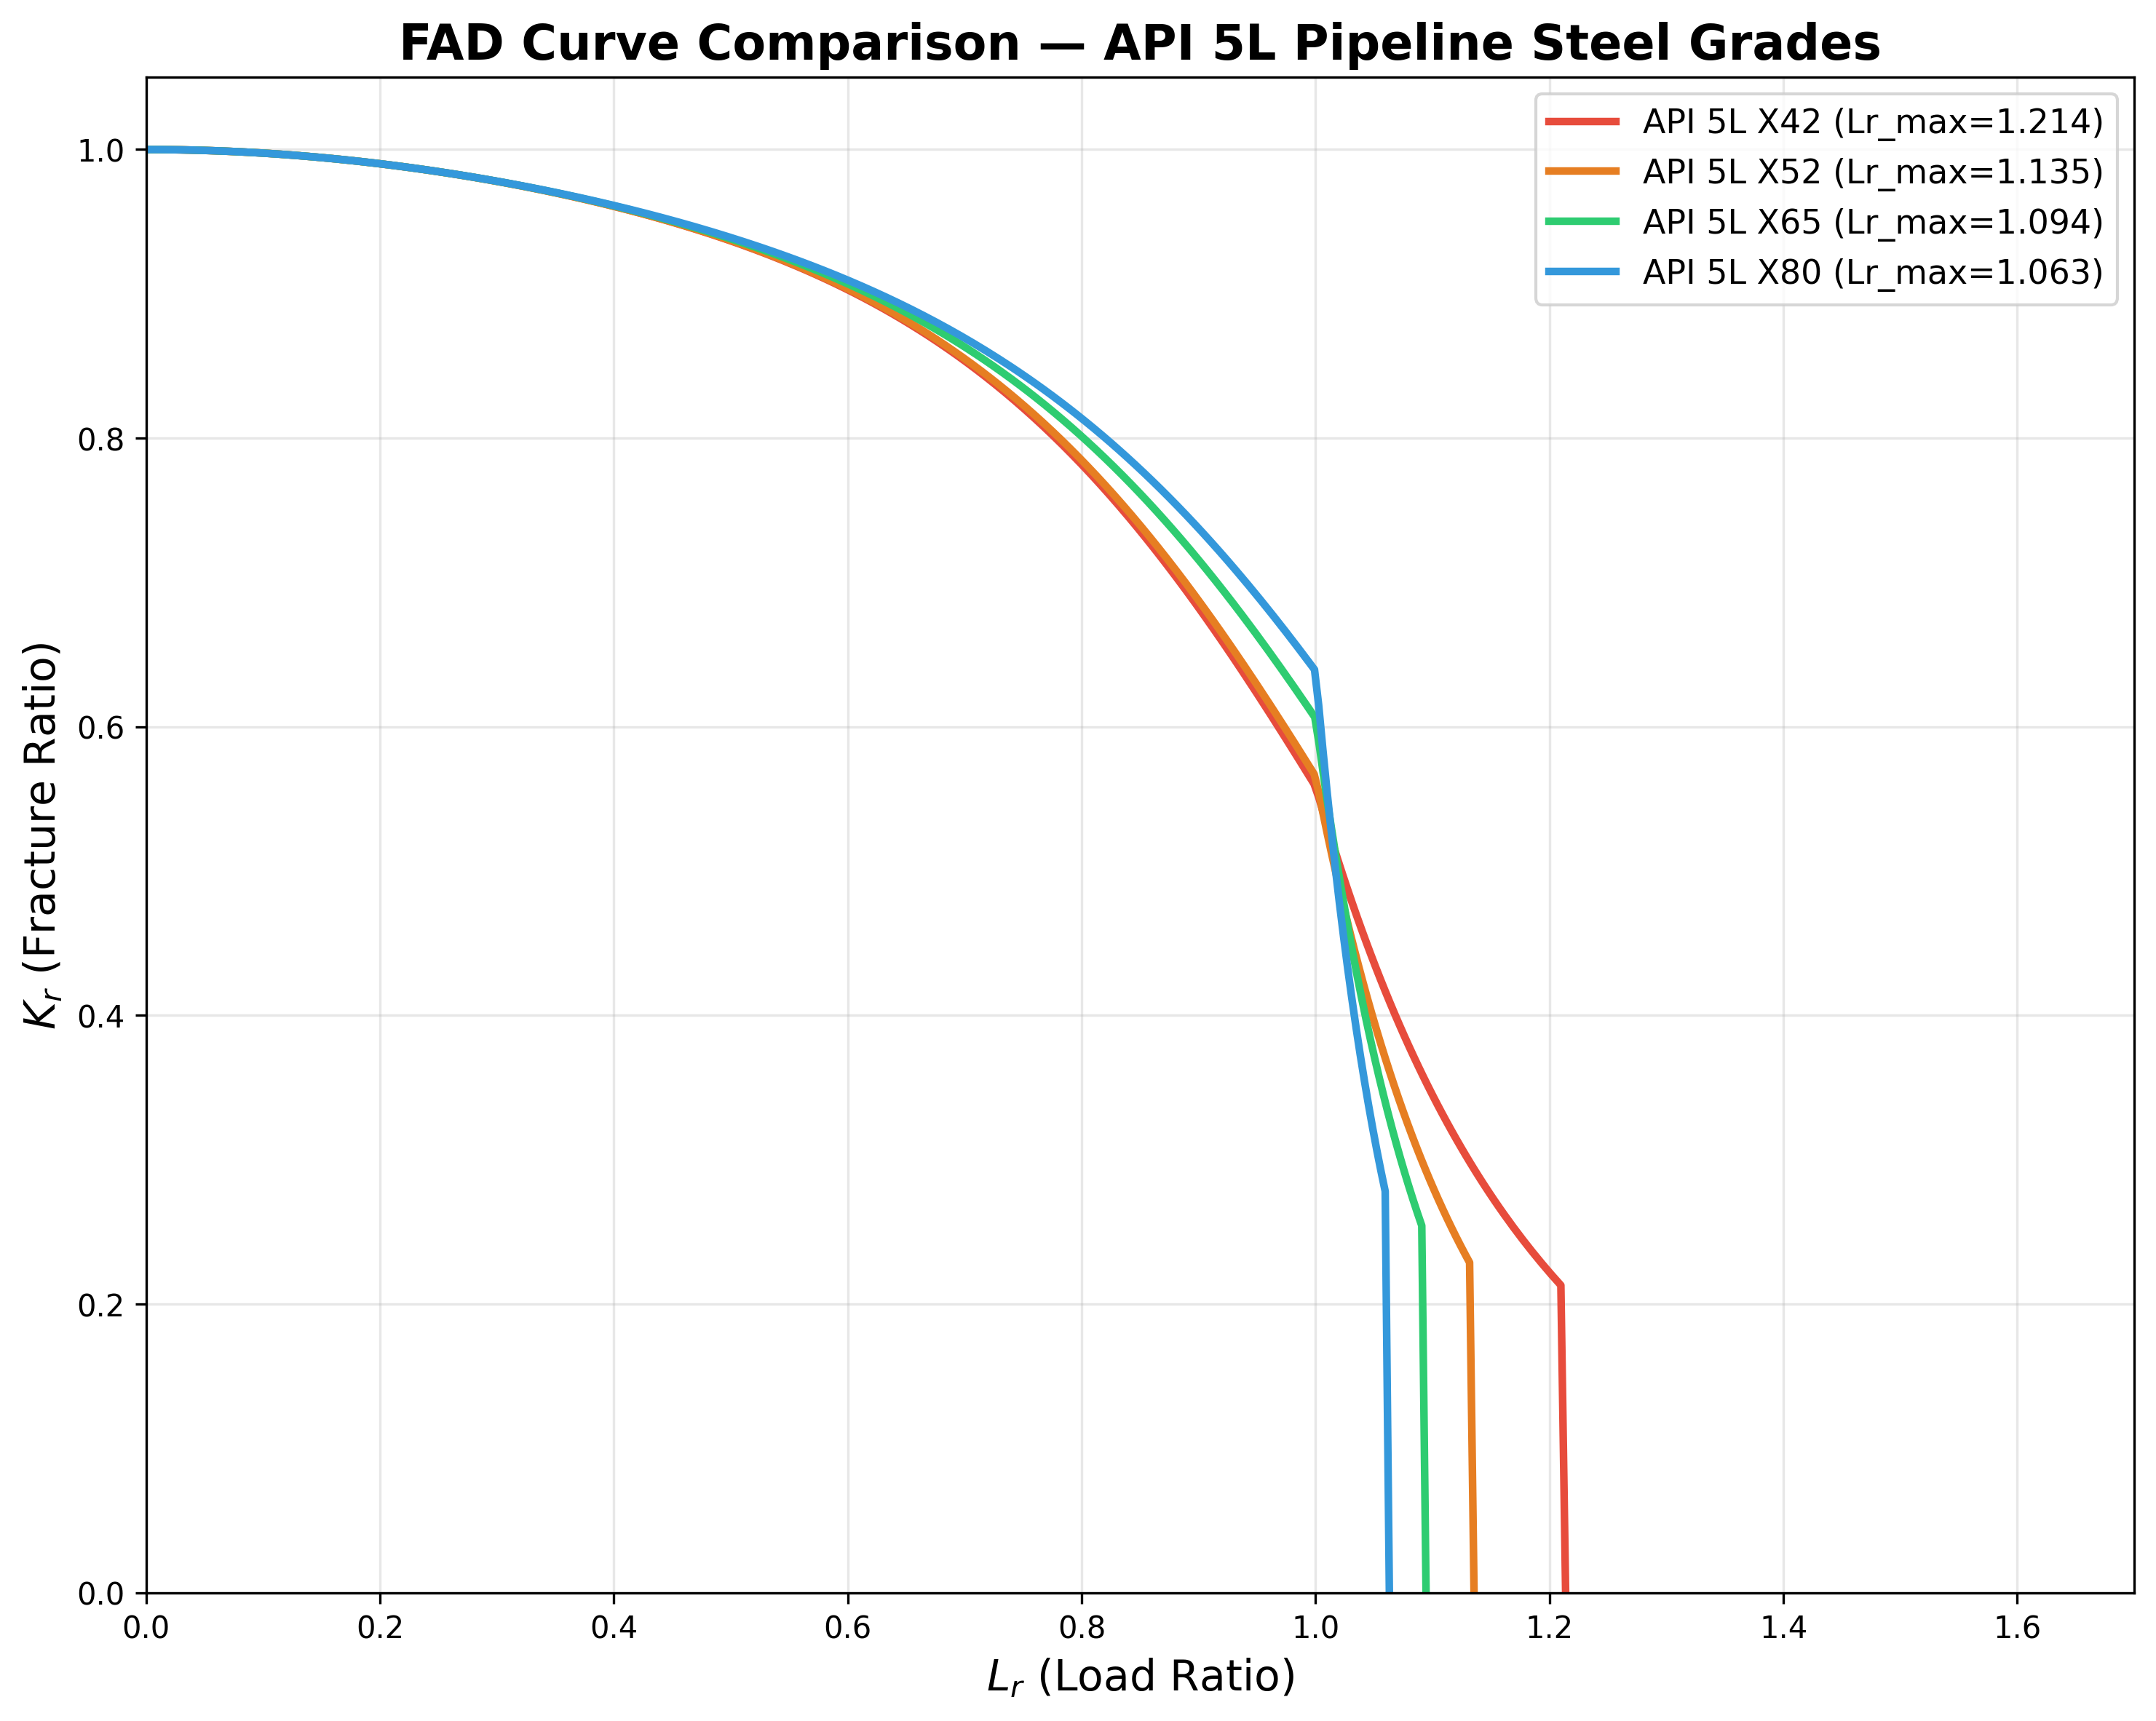
\includegraphics[width=0.78\textwidth]{fig2_fad_grade_comparison}
  \caption{BS~7910:2019 Level~2 Option~1 FAD curves for API~5L grades
    X52 through X70.  Higher yield strength shifts $L_{r,\max}$ leftward,
    reducing the acceptable load ratio range.  Assessment points for
    nominal and critical flaws are shown for X60 (primary grade in the
    Gulf Coast network model).}
  \label{fig:fad_grade_comparison}
\end{figure}

%% -----
\subsection{Fatigue Design of Welded Joints}
\label{subsec:lit_fatigue}

Fatigue failure of welded joints is governed by S-N curves of the form
$N = C \cdot \Delta\sigma^{-m}$, where $N$ is the number of cycles to
failure, $\Delta\sigma$ the stress range, and the constants $C$ and $m$
are weld-class-dependent~\cite{IIW_Fatigue:2016}.  The \ac{IIW}
Recommendations for Fatigue Design of Welded Joints and Components
codify 14 FAT classes — labelled by the characteristic fatigue strength
at $2 \times 10^6$ cycles, in megapascals — from FAT~36 (cover-plated
beams, poorest quality) to FAT~160 (smooth full-penetration welds with
post-weld machining)~\cite{IIW_Fatigue:2016,Murakami2002}.  Pipeline
girth welds qualified to API~1104:2021 acceptance criteria typically
fall in the FAT~71--FAT~90 range, depending on weld quality level and
post-weld heat treatment~\cite{API1104:2021}.

Cumulative fatigue damage is assessed through Miner's linear damage rule:
\begin{equation}
  D = \sum_i \frac{n_i}{N_i(\Delta\sigma_i)} \leq D_\mathrm{cr},
  \label{eq:miners_rule}
\end{equation}
where $n_i$ is the counted number of cycles in stress-range block $i$,
$N_i$ is the corresponding endurance life from the S-N curve, and
$D_\mathrm{cr} = 1.0$ is the critical damage sum in the IIW
formulation (conservatively reduced to $0.5$ for safety-critical
applications under variable amplitude loading)~\cite{IIW_Fatigue:2016}.

The S-N relationship exhibits a bilinear character in the high-cycle
regime: a primary inverse slope $m = 3$ for $N < 10^7$ cycles
transitions to a secondary slope $m = 5$ beyond the constant-amplitude
fatigue limit, following the IIW variable amplitude damage
model~\cite{IIW_Fatigue:2016}.  This bilinear representation reflects
the physical transition from short-crack propagation, dominated by
crack-tip plasticity and Miner accumulation, to the threshold regime
where crack closure begins to retard propagation significantly
\cite{Murakami2002,Anderson2005}.  The \texttt{fatigue\_engine.py}
module implements both slopes with the correct IIW FAT-class lookup
table, validated against published reference endurance values in the
310-test suite.

Post-weld heat treatment (\acs{PWHT}) can improve the FAT class by one
to two levels by relieving residual tensile stresses at the weld toe —
the primary crack initiation site in girth welds under axial cycling.
For in-service transmission pipelines, however, \acs{PWHT} is
operationally impractical for most repair scenarios, making the
as-welded FAT class the default for fleet-level assessments~\cite{API1104:2021,
Francis2014}.  This conservatism is embedded in the calibrated seam-type
hierarchy of \cref{tab:calibrated_scf}: fillet and lap-welded legacy
joints (pre-1970, LF-ERW, associated with poor weld quality and no
\acs{PWHT}) exhibit the highest $P_f$ values in the Monte Carlo engine.

\begin{figure}[htbp]
  \centering
  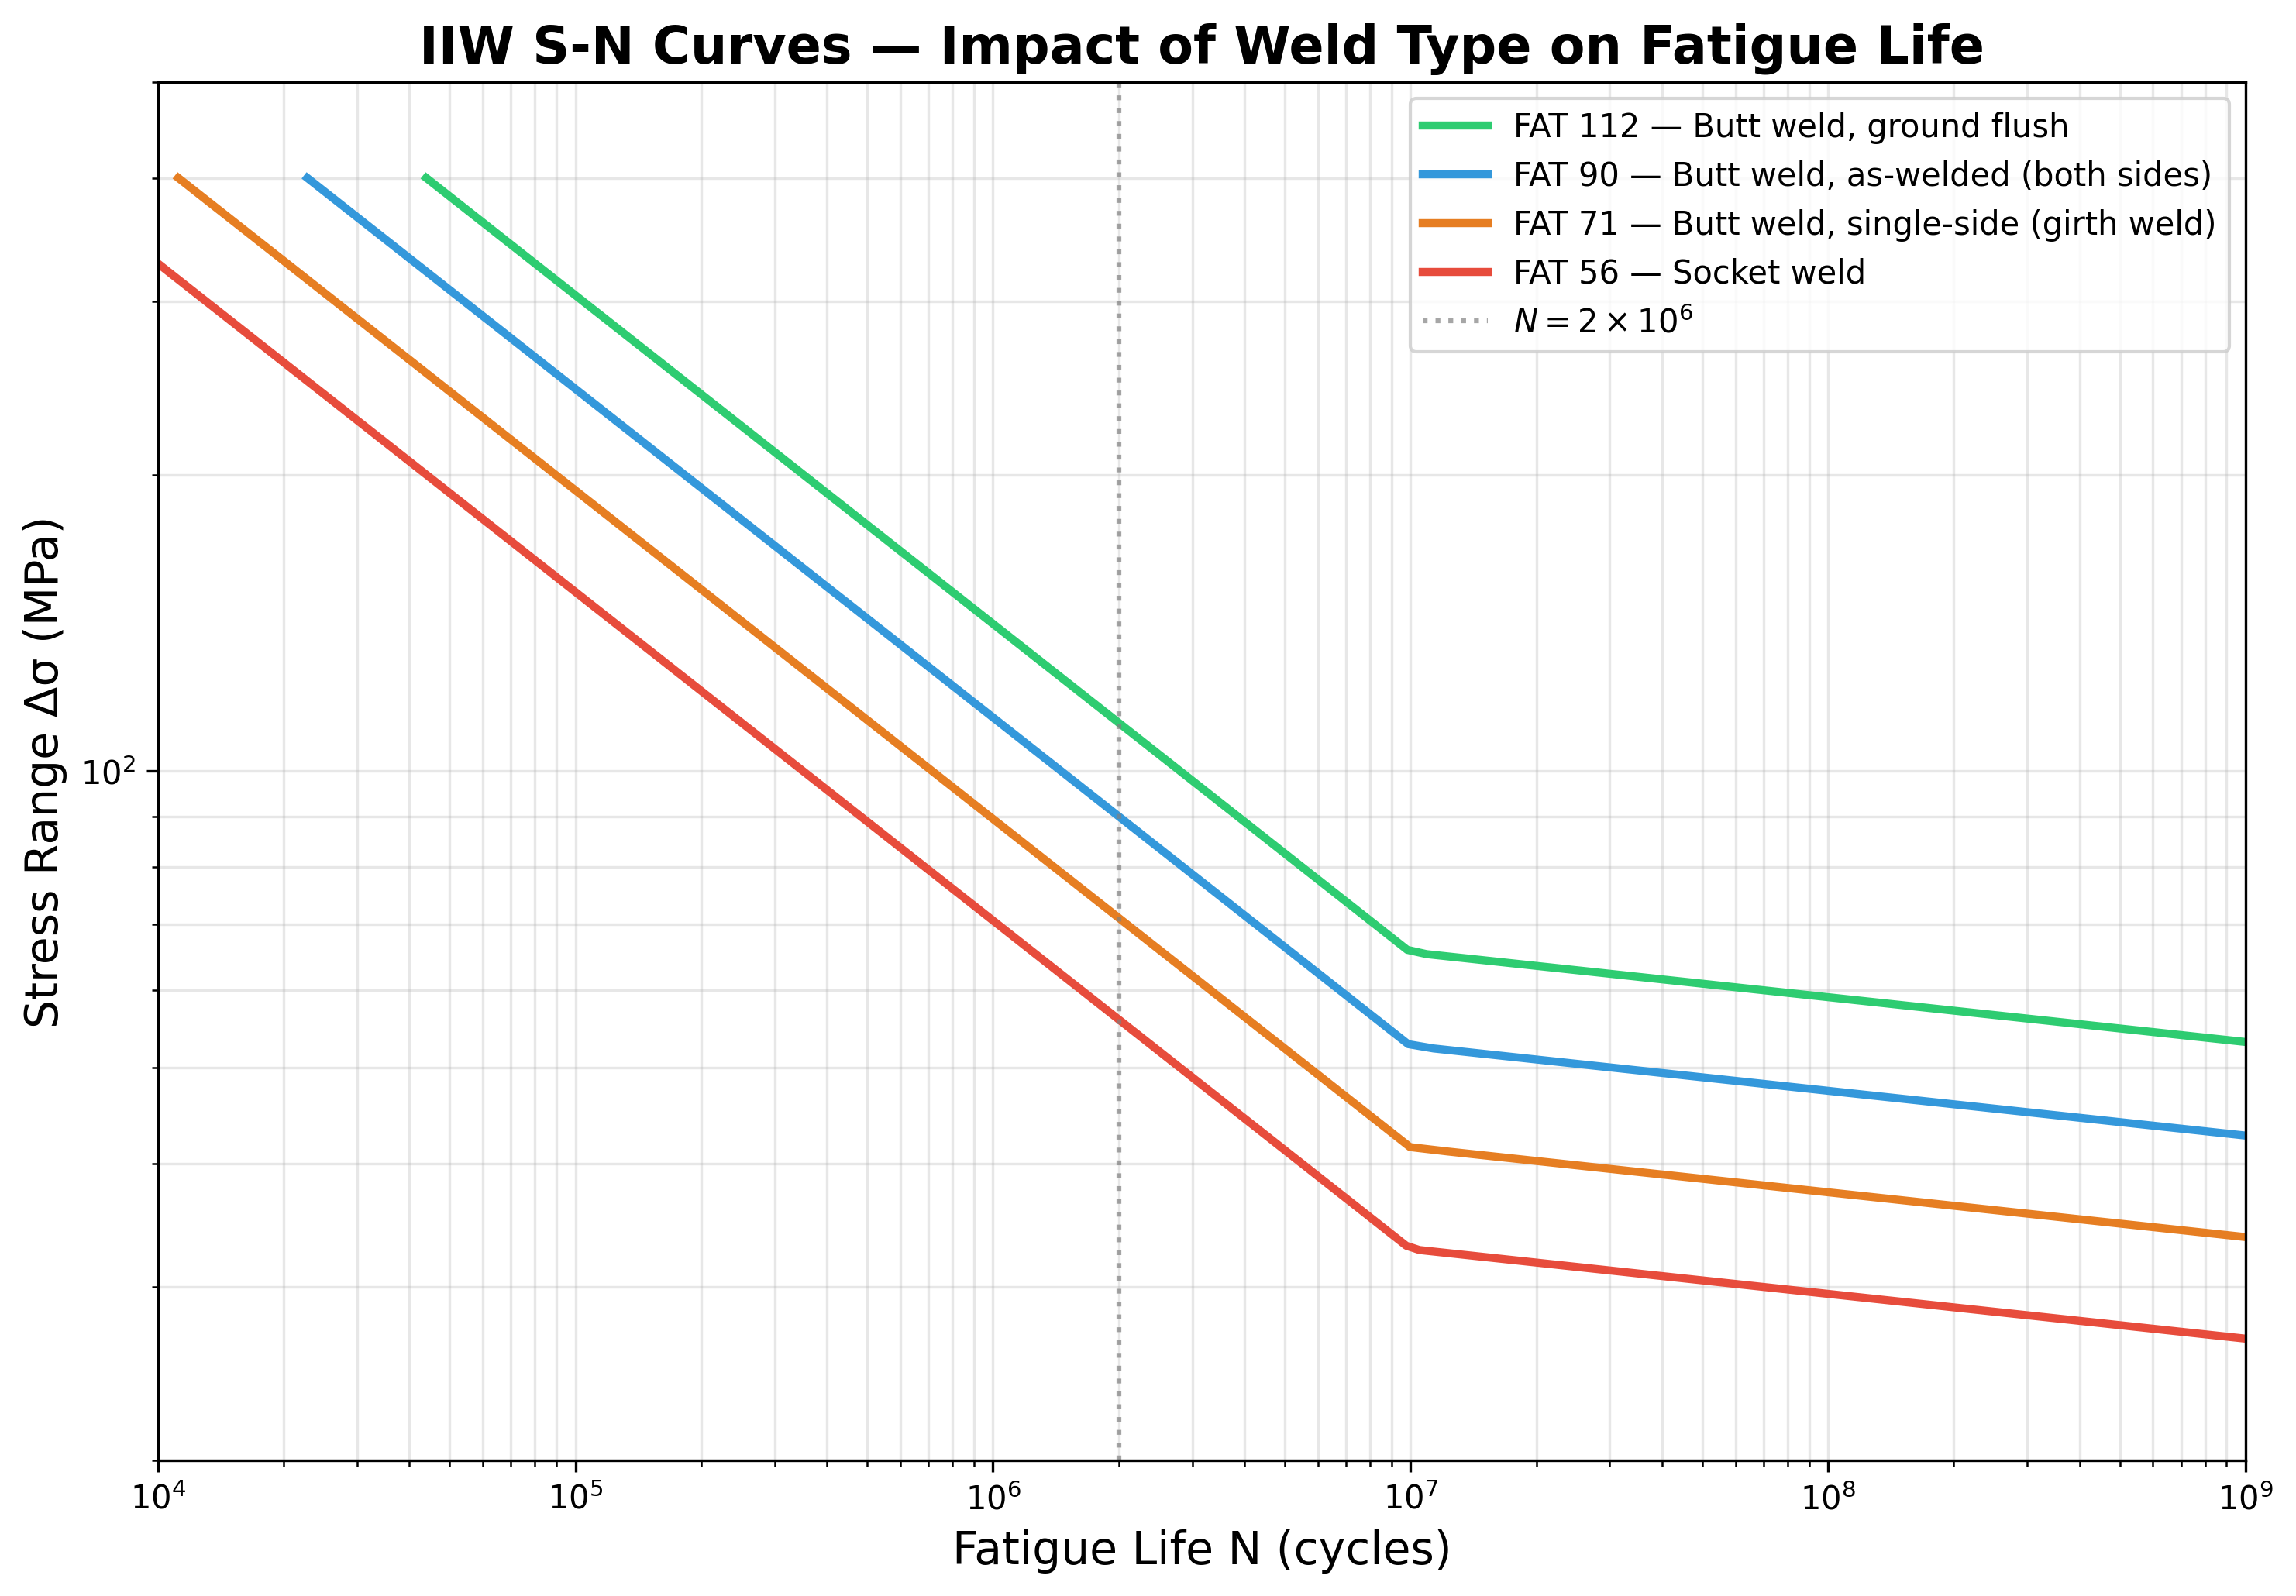
\includegraphics[width=0.82\textwidth]{fig3_sn_weld_comparison}
  \caption{IIW S-N curves for pipeline-relevant weld classes (FAT~63
    to FAT~100).  A two-order-of-magnitude spread in fatigue life exists
    at $\Delta\sigma = \SI{100}{\mega\pascal}$.  The bilinear transition
    at $N = 10^7$ cycles is evident for all classes.  Weld class
    assignments follow API~1104:2021 acceptance criteria.}
  \label{fig:sn_comparison}
\end{figure}

%% -----
\subsection{Monte Carlo Methods in Reliability Assessment}
\label{subsec:lit_mc}

Probabilistic integrity management applies \ac{MC} simulation to
propagate scatter in material properties, flaw dimensions, and operating
loads into a distribution of safety margins~\cite{Caleyo2002}.  The key
advantage over deterministic assessment is the direct quantification of
failure probability $P_f$, which is comparable against regulatory risk
tolerability criteria (typically $10^{-4}$--$10^{-6}$ per year for
high-consequence areas under \ac{ASME}~B31.8~\cite{ASME_B31_8:2025}).

Caleyo et al.~\cite{Caleyo2002} demonstrated MC integration for pipeline
corrosion growth, sampling from lognormal wall-loss distributions and
propagating to burst failure pressure.  Zhu et al.~\cite{Zhu2013}
extended the framework to strain-based design, coupling MC with
finite-element limit-load solutions for wrinkle defects.  Mo and
Li~\cite{Mo2012} applied MC to fatigue crack growth in girth welds under
variable amplitude pressure cycling, finding that SCF uncertainty
dominates the failure probability variance — a result consistent with the
sensitivity analysis in \cref{fig:pf_scf_sensitivity} of this thesis.
The present work extends this line of research to a multi-segment network
context, where individual segment $P_f$ values computed from
$N = \num{10000}$ MC trials are assembled into a NetworkX graph that
feeds directly into the Stackelberg game payoff calculation in
\cref{sec:physics_game}.

%% ------------------------------------------------------------------
\section{Security Games for Critical Infrastructure}
\label{sec:lit_games}

\subsection{Stackelberg Security Games: Foundations}
\label{subsec:lit_ssg}

A \acf{SCG} models a sequential two-player interaction where a
\emph{defender} (leader) commits to a mixed strategy $\bmc$ first,
after which an \emph{attacker} (follower) best-responds having observed
the marginal coverage probabilities~\cite{Conitzer2006}.  Under the
assumption of attacker rationality, the defender seeks a
\acf{SSE} that maximises her expected utility given the attacker's
rational best-response.  Von Stengel and Zamir established that a
Stackelberg commitment weakly dominates Nash equilibrium for the leader,
providing a rigorous game-theoretic justification for
commitment-based security protocols~\cite{Conitzer2006}.

Paruchuri et al.~\cite{Paruchuri2008} established the
\textsc{DOBSS} LP formulation for Bayesian \acp{SCG} with multiple
attacker types, in which each type $\theta \in \Theta$ is represented
by a prior probability $p_\theta$ and a utility function $\Ua^\theta(i)$.
The Bayesian expected defender utility is the prior-weighted average of
type-conditional utilities at the rational best-response target.
Because the follower best-response is a piecewise function of the
leader's mixed strategy, the problem is non-convex in general;
\textsc{DOBSS} linearises it via an enumeration of candidate optimal
attacker targets, solving one LP per target and selecting the global
optimum~\cite{Paruchuri2008}.  This approach scales polynomially in the
number of targets $n$ and attack types $|\Theta|$, making it tractable
for the 22-target, 3-type instance in \cref{ch:physics}.

Korzhyk et al.~\cite{Korzhyk2011} subsequently showed that under mild
conditions on the utility structure (unique attacker best-response), the
Stackelberg value equals the Nash equilibrium value of the zero-sum
game, providing a mathematical bridge between the two solution concepts.
This result is exploited in \cref{subsec:physics_lp} to establish the
uniqueness of the LP-derived SSE for the physics-informed payoff structure.

\subsection{Deployed Systems}
\label{subsec:lit_deployed}

Real-world deployments have demonstrated that SSG-based patrol scheduling
can meaningfully reduce adversarial incident rates.  ARMOR randomised
K-9 unit and police patrol routes across the four terminals of Los Angeles
International Airport~\cite{An2013}; a post-deployment evaluation by the
\ac{TSA} reported a statistically significant reduction in security
anomalies relative to the human-scheduled baseline.  PROTECT scheduled
U.S.\ Coast Guard patrol vessels along Boston Harbour ferry routes,
incorporating three adversary models — opportunistic, capable, and
sophisticated — analogous to the three attacker types (STRATEGIC,
OPPORTUNISTIC, STATE\_ACTOR) in this thesis~\cite{Tambe2011}.  IRIS
randomised U.S.\ Federal Air Marshal seat assignments on domestic flights,
demonstrating deployment at a national scale with real operational constraints~\cite{Tambe2011}.

A structural limitation shared by all deployed systems is that attacker
payoffs are supplied by subject-matter experts as scalar constants,
without formal derivation from structural or physical models of the
protected assets.  A technically sophisticated adversary who understands
that a fillet-welded legacy joint at maximum operating pressure has
$P_f \approx \num{0.88}$ while a seamless segment has $P_f \approx
\num{0.53}$ — a fourfold difference in consequence-weighted failure
probability per unit of attack effort — will exploit the gap between
the expert-estimated payoffs and physical reality.  The physics-informed
payoff structure developed in \cref{ch:physics} closes this gap directly.

\subsection{Critical Infrastructure and Network Attacks}
\label{subsec:lit_ci}

Network-theoretic analysis of critical infrastructure~\cite{Newman2010,
Albert2000} demonstrates that real-world infrastructure graphs exhibit
scale-free degree distributions, and removal of a small number of
high-betweenness nodes causes disproportionate disruption to global
network connectivity~\cite{Albert2000}.  Brown et al.~\cite{Brown2006}
applied bilevel optimisation to find the worst-case interdiction set for
electric power grids; Lewis~\cite{Lewis2014} extended the framework to
interdependent pipeline and power systems, showing that cascading failures
initiated at pipeline compression stations can propagate to wide-area
power outages.

A key limitation of purely network-theoretic interdiction models is the
assumption of structural equivalence across edges: an attacker maximising
betweenness disruption ignores whether the target pipe segment is likely
to fail under the applied attack mode.  Conversely, a purely structural
approach minimising $P_f$ ignores the network consequence of a given
failure.  The Bayesian SSG payoff structure in this thesis explicitly
combines both dimensions: the STATE\_ACTOR type is parameterised to
weight both $P_f$ and betweenness centrality, while the STRATEGIC type
prioritises asset value and the OPPORTUNISTIC type exploits structural
weakness alone.

%% ------------------------------------------------------------------
\section{Adversarial Machine Learning and NDE Security}
\label{sec:lit_adv}

\subsection{Adversarial Attacks on Neural Networks}
\label{subsec:lit_adv_basics}

Szegedy et al.~\cite{Szegedy2014} first demonstrated that small,
imperceptible perturbations to input features can cause deep neural
networks to misclassify with high confidence.  The underlying mechanism
is the geometry of high-dimensional decision boundaries: in feature
spaces of dimension $d \gg 1$, class boundaries are dense, and the
distance from a correctly classified point to the nearest misclassified
region is $\mathcal{O}(1/\sqrt{d})$ for random inputs, shrinking with
problem dimensionality~\cite{Goodfellow2016}.  Goodfellow et al.\
proposed the \acf{FGSM}~\cite{Goodfellow2015}:
\begin{equation}
  \bm{x}^\mathrm{adv} = \bm{x} + \eps \cdot \mathrm{sign}
    \!\left(\nabla_{\bm{x}} \mathcal{L}(\theta, \bm{x}, y)\right),
  \label{eq:fgsm}
\end{equation}
which adds a single signed gradient step bounded in $L_\infty$ norm by
$\eps$.  The key insight is that the gradient direction, not its
magnitude, determines the adversarial perturbation, making FGSM
computationally efficient for any differentiable loss.

Kurakin et al.~\cite{Kurakin2017} extended FGSM to the iterative
\ac{BIM}, applying $T$ small FGSM steps with $L_\infty$ projection
after each iteration.  BIM generally achieves higher attack success
rates than FGSM at the same $\eps$ budget, though at greater
computational cost.  Madry et al.~\cite{Madry2018} formalised \ac{PGD}
— BIM initialised from a random perturbation within the $L_\infty(\eps)$
ball — as the canonical strongest first-order attack under the $L_\infty$
threat model.  A classifier trained to resist PGD perturbations
(adversarial training) is provably robust to all first-order attacks
within the same threat model~\cite{Madry2018}.  The observation in
\cref{ch:adversarial} that BIM outperforms PGD on the NDE feature set
(ASR $\num{20.1}\% > \num{9.4}\%$) reveals an important domain-specific
deviation from the standard ordering: local gradient curvature, not
random initialisation, dominates in the structured 32-dimensional NDE
feature space.

Carlini and Wagner~\cite{Carlini2017} subsequently showed that many
first-generation defences — input preprocessing, detection networks —
can be circumvented by stronger optimisation-based attacks.  This raises
the bar for what constitutes genuine adversarial robustness in
safety-critical applications, and motivates the quantitative ASR
measurements in \cref{ch:adversarial} rather than qualitative
robustness claims.

\subsection{Machine Learning for NDE}
\label{subsec:lit_nde_ml}

Deep learning methods have been applied to automated weld defect
classification from radiographic~\cite{Munir2019} and ultrasonic
inspection data~\cite{Meyendorf2022}.  Munir et al.~\cite{Munir2019}
achieved $>97\%$ accuracy on a four-class weld defect radiograph dataset
using a ResNet-50 backbone, demonstrating that production-grade
classification accuracy is achievable with moderate training sets.
Meyendorf et al.~\cite{Meyendorf2022} reviewed the state of AI-assisted
NDE, identifying ultrasonic phased-array imaging and time-of-flight
diffraction as the modalities with the most mature ML integration.

Despite this accuracy progress, adversarial robustness of NDE
classifiers has received virtually no treatment in the open literature.
The closest structural analogue is the medical imaging domain, where
adversarial perturbations have been shown to cause misdiagnosis of
malignant lesions as benign — a direct analogue to the CRACK $\to$ CLEAN
misclassification scenario in \cref{ch:adversarial}~\cite{Goodfellow2016}.
The present thesis is, to the author's knowledge, the first to
characterise adversarial attack success rates for an NDE weld defect
classifier and to connect those rates quantitatively to the game-theoretic
consequence of a missed defect through the physics-informed payoff structure.

%% ------------------------------------------------------------------
\section{The Unifying Gap}
\label{sec:lit_gap}

Three decades of structural integrity research have produced rigorous,
standards-backed tools for computing $P_f$ from physical first principles.
Two decades of security game research have produced deployable algorithms
for optimal defender resource allocation.  A decade of adversarial ML
research has characterised the fragility of neural-network inspection
systems.  No published work combines all three into a single, coherent,
end-to-end framework.  \Cref{tab:lit_comparison} summarises the research
landscape and positions this thesis.

\begin{table}[htbp]
  \centering
  \caption{Positioning of this thesis relative to the existing literature.
    A tick (\checkmark) indicates the capability is present;
    a dash (---) indicates it is absent.  No prior work satisfies all
    four requirements simultaneously.}
  \label{tab:lit_comparison}
  \begin{tabular}{@{}lcccc@{}}
    \toprule
    Work & Physics $\Pf$ & SSG payoff & Network & Adversarial NDE \\
    \midrule
    BS~7910 / API~579~\cite{BS7910:2019,API579:2021}
      & \checkmark & --- & --- & --- \\
    ARMOR / PROTECT~\cite{An2013,Tambe2011}
      & --- & \checkmark & --- & --- \\
    Brown et al.~\cite{Brown2006}
      & --- & --- & \checkmark & --- \\
    Munir et al.~\cite{Munir2019}
      & --- & --- & --- & ---\textsuperscript{$a$} \\
    Madry et al.~\cite{Madry2018}
      & --- & --- & --- & \checkmark \\
    \textbf{This thesis}
      & \checkmark & \checkmark & \checkmark & \checkmark \\
    \bottomrule
    \multicolumn{5}{@{}l}{\textsuperscript{$a$}High accuracy achieved; adversarial robustness not assessed.}
  \end{tabular}
\end{table}

The specific gap this thesis fills is twofold.  First, no prior security
game formulation for pipeline infrastructure derives attacker payoffs
from physics-based failure probability: existing models assign payoffs
heuristically, creating exploitable information asymmetry for a
technically sophisticated adversary.  Second, no prior work treats
adversarial manipulation of NDE inspection outputs as a strategic
layer within a game-theoretic resource allocation framework, despite the
direct operational pathway from suppressed defect detection to
undefended physical vulnerability.  Stated formally:

\begin{quote}
  \textit{The absence of a physics-grounded payoff function in Bayesian
  Stackelberg security games for pipeline infrastructure, and the
  consequent absence of any treatment of adversarial NDE manipulation
  as a strategic layer within such games.}
\end{quote}

\noindent The following chapter constructs the remedy, beginning with
the PHMSA empirical calibration that grounds all subsequent quantitative
claims in real fleet incident data.


%% ---------------------------------------------------------------
%%  CHAPTER 3 — PHYSICS-INFORMED VULNERABILITY ENGINE (ZONE C)
%% ---------------------------------------------------------------
%% ============================================================
%% CHAPTER 3 — PHYSICS-INFORMED VULNERABILITY ENGINE (ZONE C)
%% ============================================================

\chapter{Physics-Informed Vulnerability Engine}
\label{ch:physics}

\section{Chapter Overview}
\label{sec:physics_overview}

This chapter develops the three interconnected layers of Zone~C:
(i) the \ac{MC} failure probability engine grounded in \ac{BS7910}:2019
and \acs{IIW} fatigue standards (\cref{sec:physics_mc}),
(ii) the Gulf Coast pipeline network model with physics-derived edge
attributes (\cref{sec:physics_network}), and
(iii) the Bayesian Stackelberg Security Game with LP-enumeration solver
(\cref{sec:physics_game}).  All numerical results in this chapter are
derived from the validated codebase and cross-checked against the
310-test suite described in the Technical Inventory.

\section{PHMSA Empirical Calibration}
\label{sec:physics_phmsa}

\subsection{Dataset}
\label{subsec:physics_phmsa_data}

The probabilistic inputs to the failure model are calibrated against the
\ac{PHMSA} Gas Transmission and Gathering Pipeline Annual Report
dataset~\cite{PHMSA2024}, comprising \num{1996} incident records spanning
2010--2024, with 624 data fields per record.  Filtering for material
and weld-related failure causes yields 216 events with usable seam-type
and material-grade information.

% Figure placeholder
\begin{figure}[htbp]
  \centering
  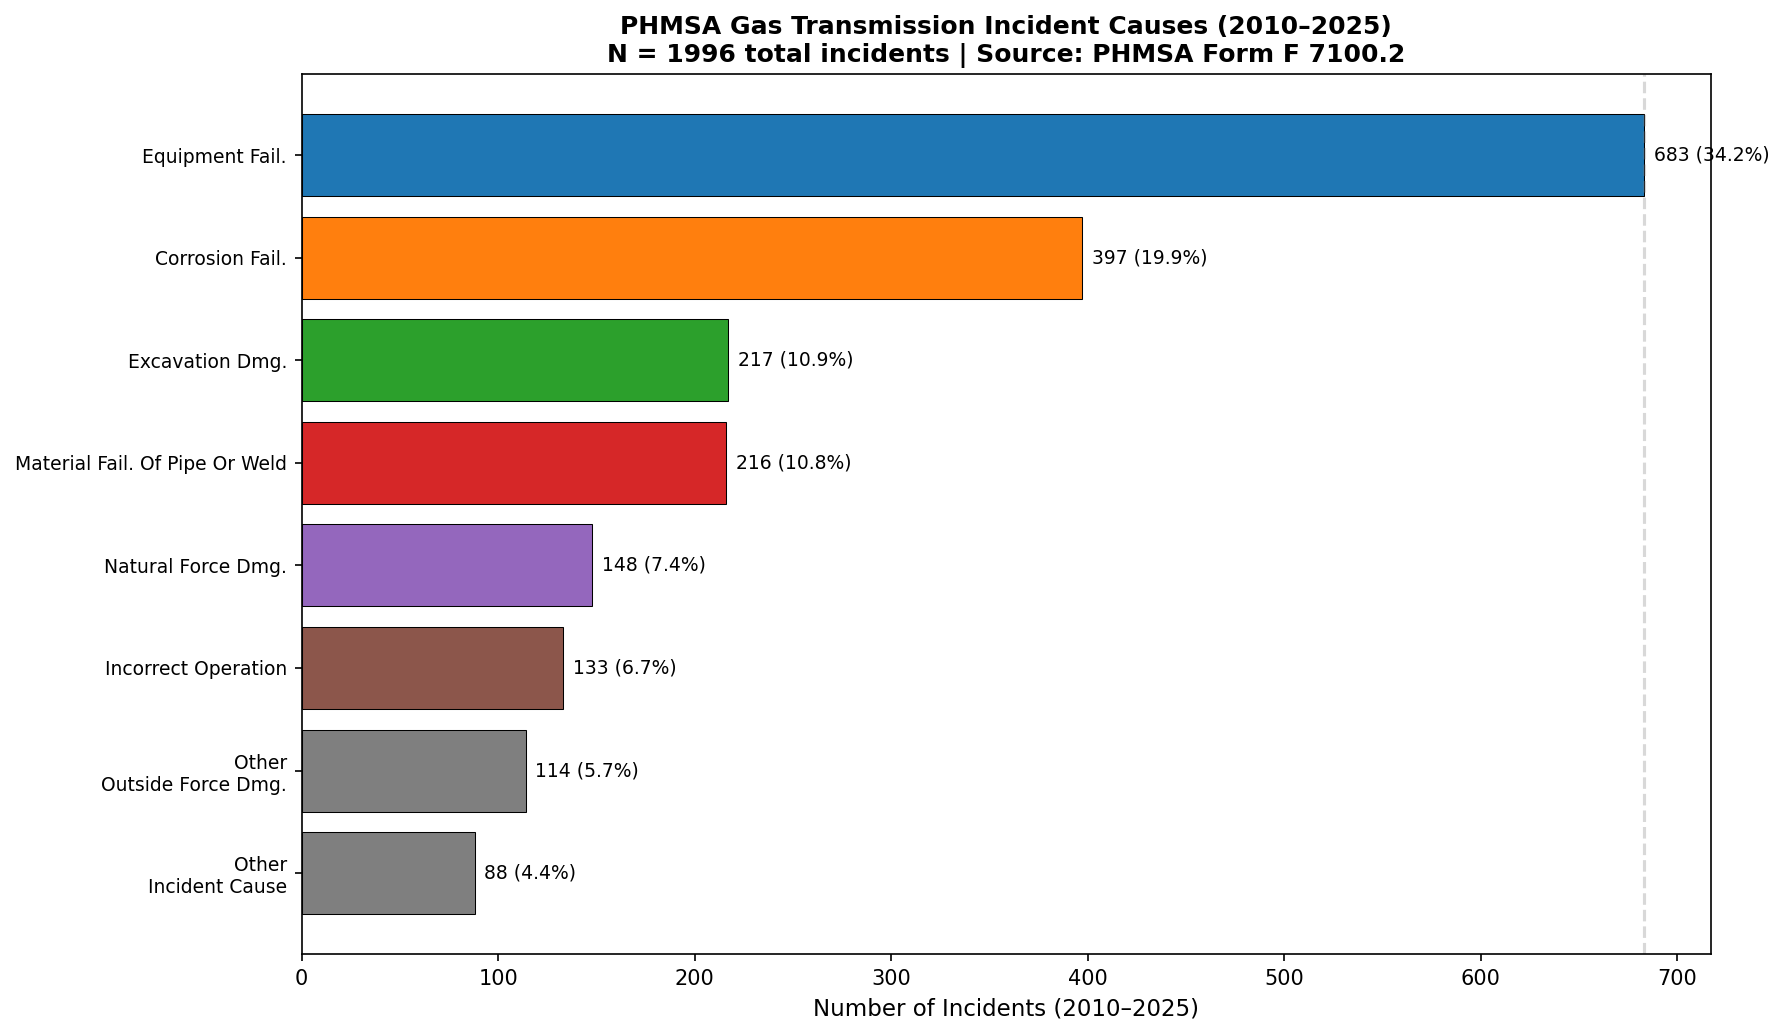
\includegraphics[width=0.92\textwidth]{fig6_phmsa_cause_distribution}
  \caption{Distribution of incident causes in the PHMSA Gas Transmission
    dataset (2010--2024, $n = \num{1996}$).  Material and weld-related
    failures account for \SI{10.8}{\percent} of all recorded incidents
    and represent the highest-consequence category by median consequence
    cost.}
  \label{fig:phmsa_cause}
\end{figure}

\subsection{Calibrated Distributions}
\label{subsec:physics_calibration}

\Cref{tab:calibrated_scf} presents the \acs{SCF} values and associated
coefficient of variation ($c_v$) calibrated from the PHMSA data for
each seam type.  The lognormal parameterisation follows the standard
practice for material scatter in fracture assessment~\cite{BS7910:2019,
Anderson2005}.

\begin{table}[htbp]
  \centering
  \caption{Calibrated Stress Concentration Factors by Seam Type
    (PHMSA-informed, BS~7910:2019 reference values in parentheses).
    All values are mean $\pm$ one standard deviation.}
  \label{tab:calibrated_scf}
  \begin{tabular}{@{}lcccc@{}}
    \toprule
    Seam Type & $\mu_\mathrm{SCF}$ & $\sigma_\mathrm{SCF}$ &
    $c_v$ & Mean $\Pf$ \\
    \midrule
    Seamless              & 1.00 & 0.05 & 0.050 & 0.53 \\
    DSAW                  & 1.25 & 0.10 & 0.080 & 0.62 \\
    HF-ERW                & 1.50 & 0.15 & 0.100 & 0.66 \\
    LF-ERW (pre-1970)     & 1.80 & 0.20 & 0.111 & 0.74 \\
    Spiral SAW            & 1.40 & 0.12 & 0.086 & 0.64 \\
    Fillet / Lap-welded   & 2.20 & 0.25 & 0.114 & 0.88 \\
    \bottomrule
  \end{tabular}
\end{table}

\section{BS 7910 Failure Assessment Diagram Engine}
\label{sec:physics_fad}

\subsection{Option 1 FAD Curve}
\label{subsec:physics_fad_curve}

The BS~7910:2019 Level~2 Option~1 \ac{FAD} curve is defined by
\cite{BS7910:2019}:
\begin{equation}
  f(\Lr) = \left[1 + 0.5\,\Lr^2\right]^{-1/2}
    \left(0.3 + 0.7\,\mathrm{e}^{-\mu\,\Lr^6}\right),
    \qquad 0 \leq \Lr \leq \Lr^\mathrm{max},
  \label{eq:fad_option1}
\end{equation}
where $\mu = \min(0.001\,E/\sigma_y,\; 0.6)$ and the cut-off
$\Lr^\mathrm{max} = (\sigma_y + \sigma_u)/(2\sigma_y)$.  A flaw is
acceptable if and only if the assessment point $(\Lr, \Kr)$ lies within
the envelope defined by \cref{eq:fad_option1}.

% Figure placeholder
\begin{figure}[htbp]
  \centering
  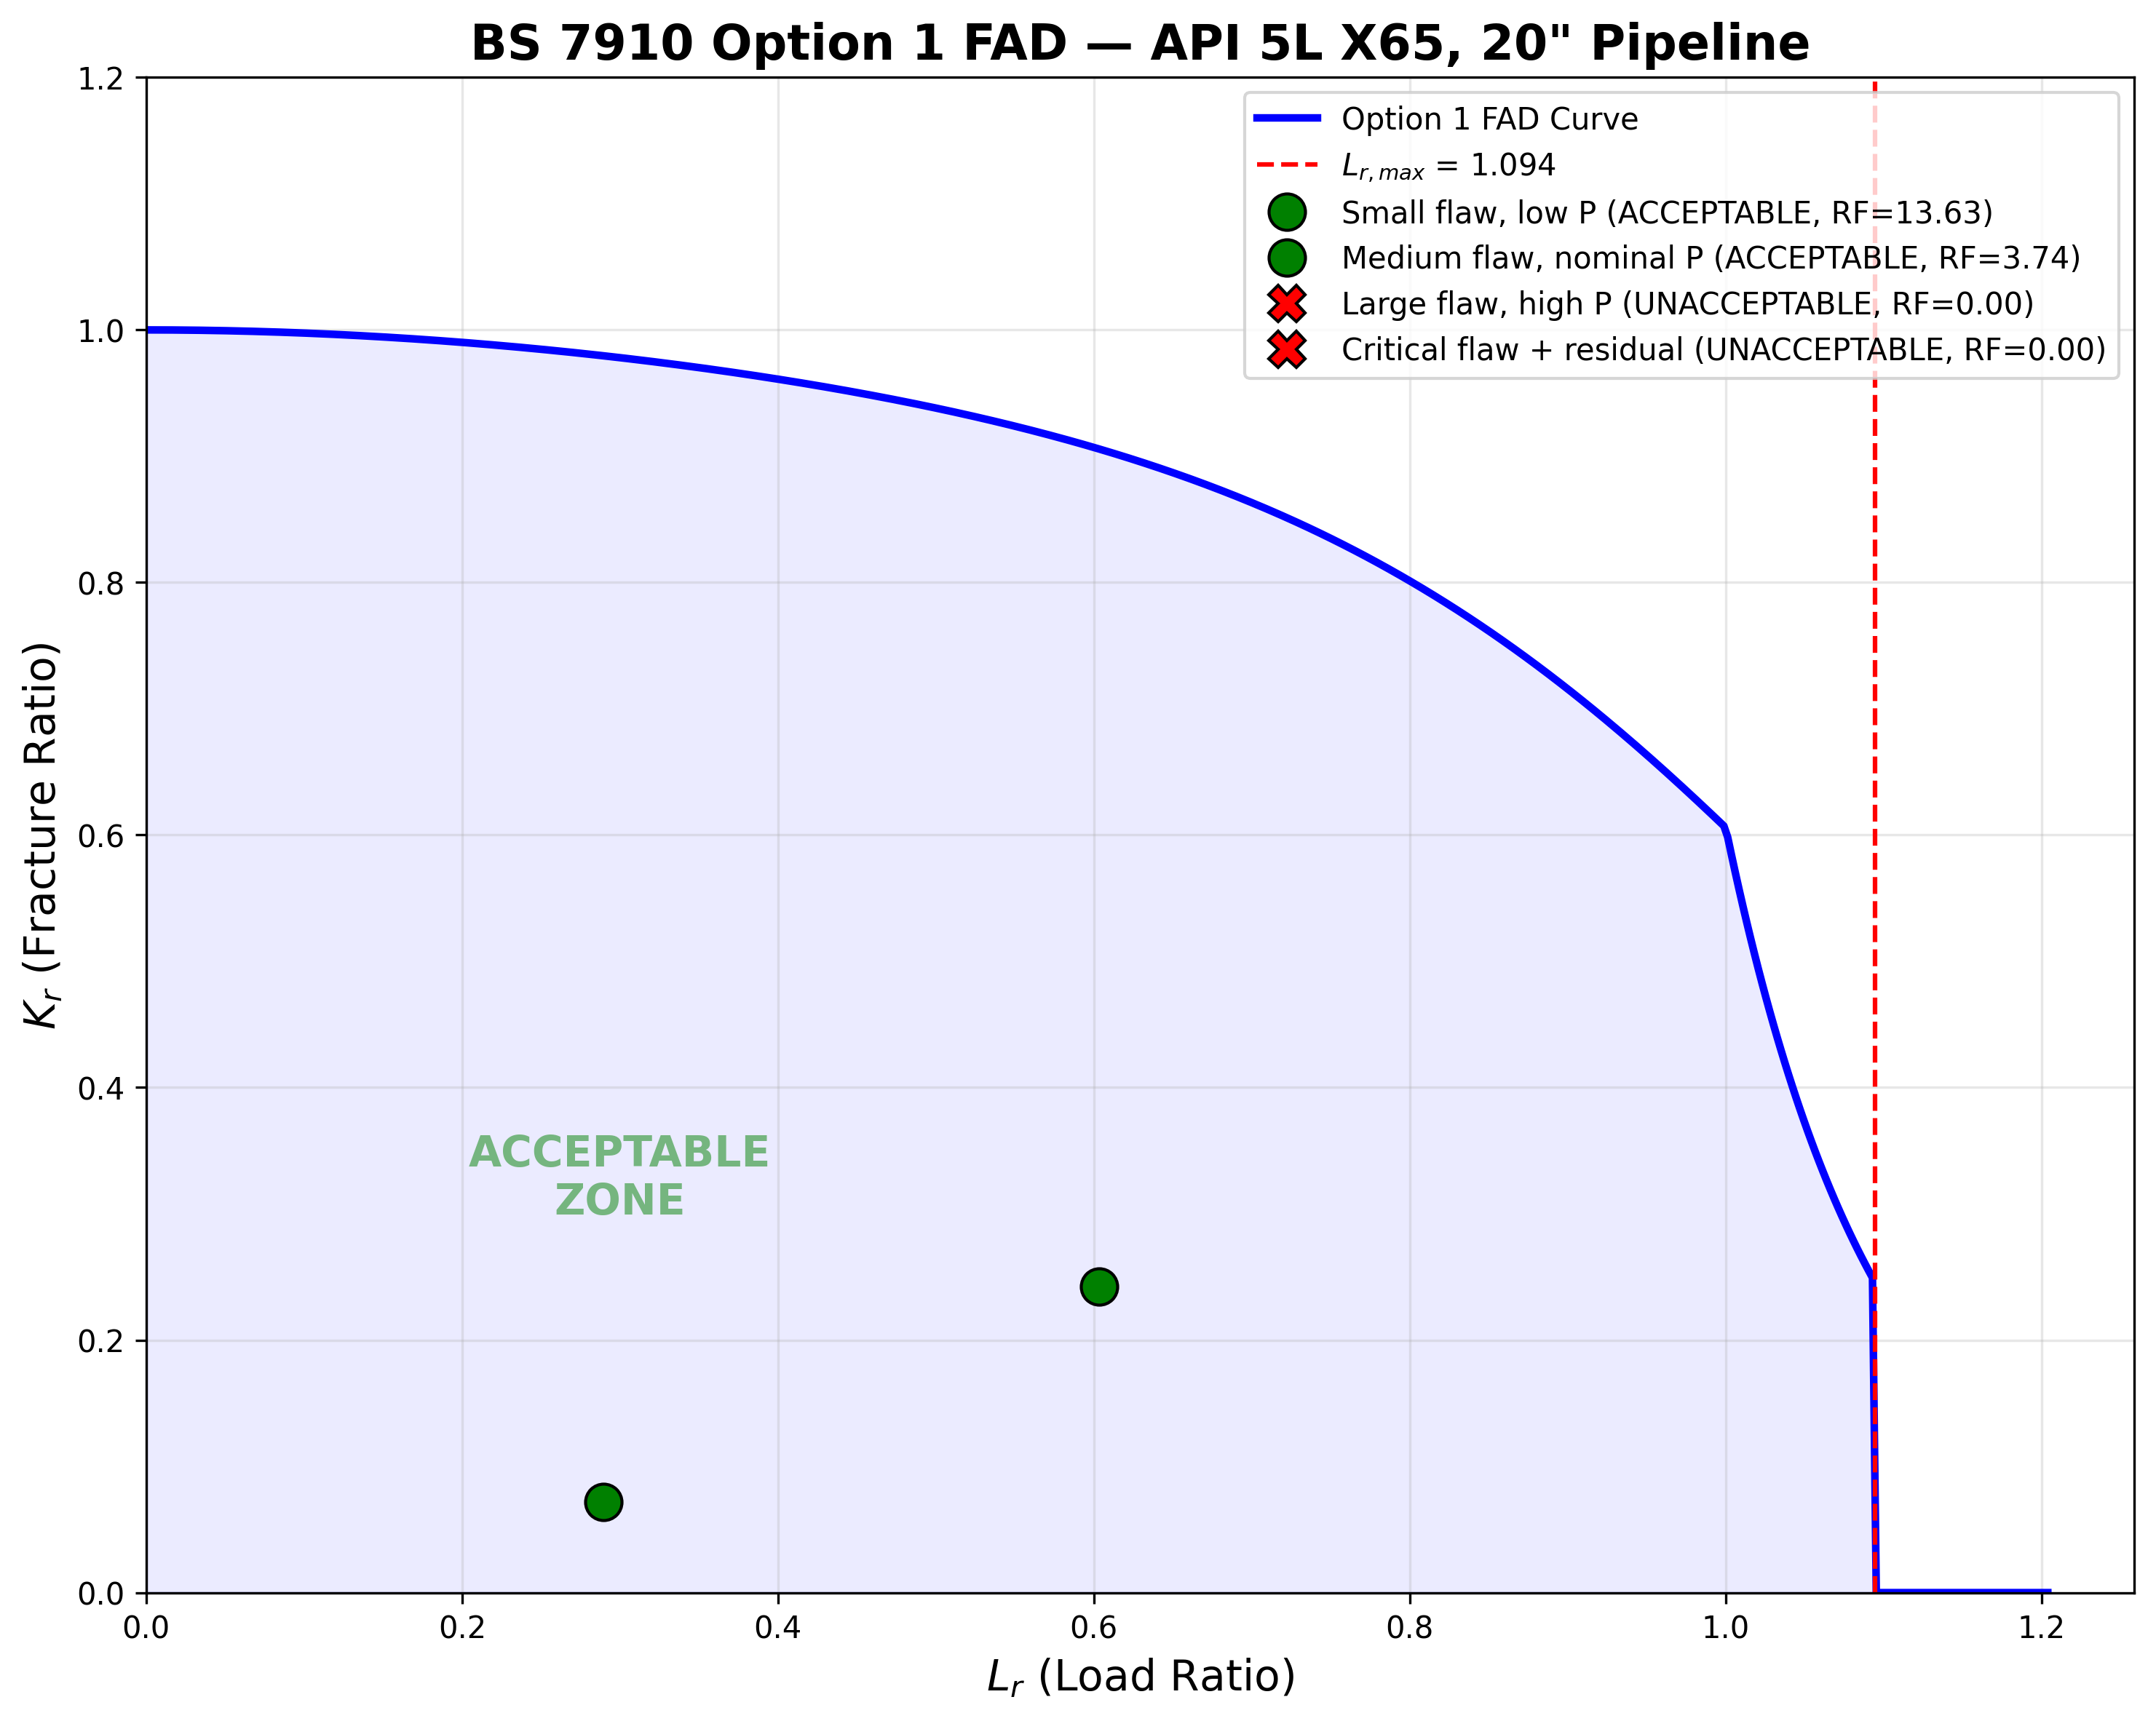
\includegraphics[width=0.80\textwidth]{fig1_fad_assessment}
  \caption{BS~7910:2019 Level~2 Option~1 Failure Assessment Diagram for
    an API~5L X60 seamless segment.  The nominal assessment point (circle,
    green) lies inside the safe region.  The critical assessment point
    (diamond, red) is outside the FAD envelope, indicating fracture
    instability.  Operating conditions: MAOP at \SI{72}{\percent} SMYS.}
  \label{fig:fad_assessment}
\end{figure}

\subsection{Toughness and Load Ratios}
\label{subsec:physics_kr_lr}

The fracture ratio is $\Kr = K_\mathrm{I} / K_\mathrm{mat}$, where
$K_\mathrm{I}$ is computed from the stress intensity solution for a
surface crack in a cylindrical shell~\cite{BS7910:2019}, and
$K_\mathrm{mat}$ is the characteristic fracture toughness.  The load
ratio $\Lr = \sigma_\mathrm{ref}/\sigma_y$ uses the reference stress
solution for an axial surface flaw~\cite{BS7910:2019,API579:2021}.
Applied stresses assume \ac{MAOP} loading at
\SI{72}{\percent}~\acs{SMYS}, consistent with \acs{ASME}~B31.8:2025
design basis~\cite{ASME_B31_8:2025}.

\section{Monte Carlo Failure Probability Engine}
\label{sec:physics_mc}

\subsection{Simulation Design}
\label{subsec:physics_mc_design}

For each pipeline segment $e$, $N = \num{10000}$ independent realisations
of the material and flaw-geometry random variables are drawn, and the
FAD acceptability criterion is evaluated for each trial:
\begin{equation}
  \Pf(e) = \frac{1}{N}\sum_{k=1}^{N}
    \mathbf{1}\!\left[\Kr^{(k)} > f\!\left(\Lr^{(k)}\right)
    \;\mathrm{or}\;
    \Lr^{(k)} \geq \Lr^\mathrm{max}\right].
  \label{eq:mc_pf}
\end{equation}
Material properties ($\sigma_y$, $E$, $K_\mathrm{mat}$) follow lognormal
distributions with parameters from \cref{tab:calibrated_scf}.  Flaw
dimensions follow truncated normal distributions bounded by API~1104:2021
acceptance criteria~\cite{API1104:2021}.

% Figure placeholder
\begin{figure}[htbp]
  \centering
  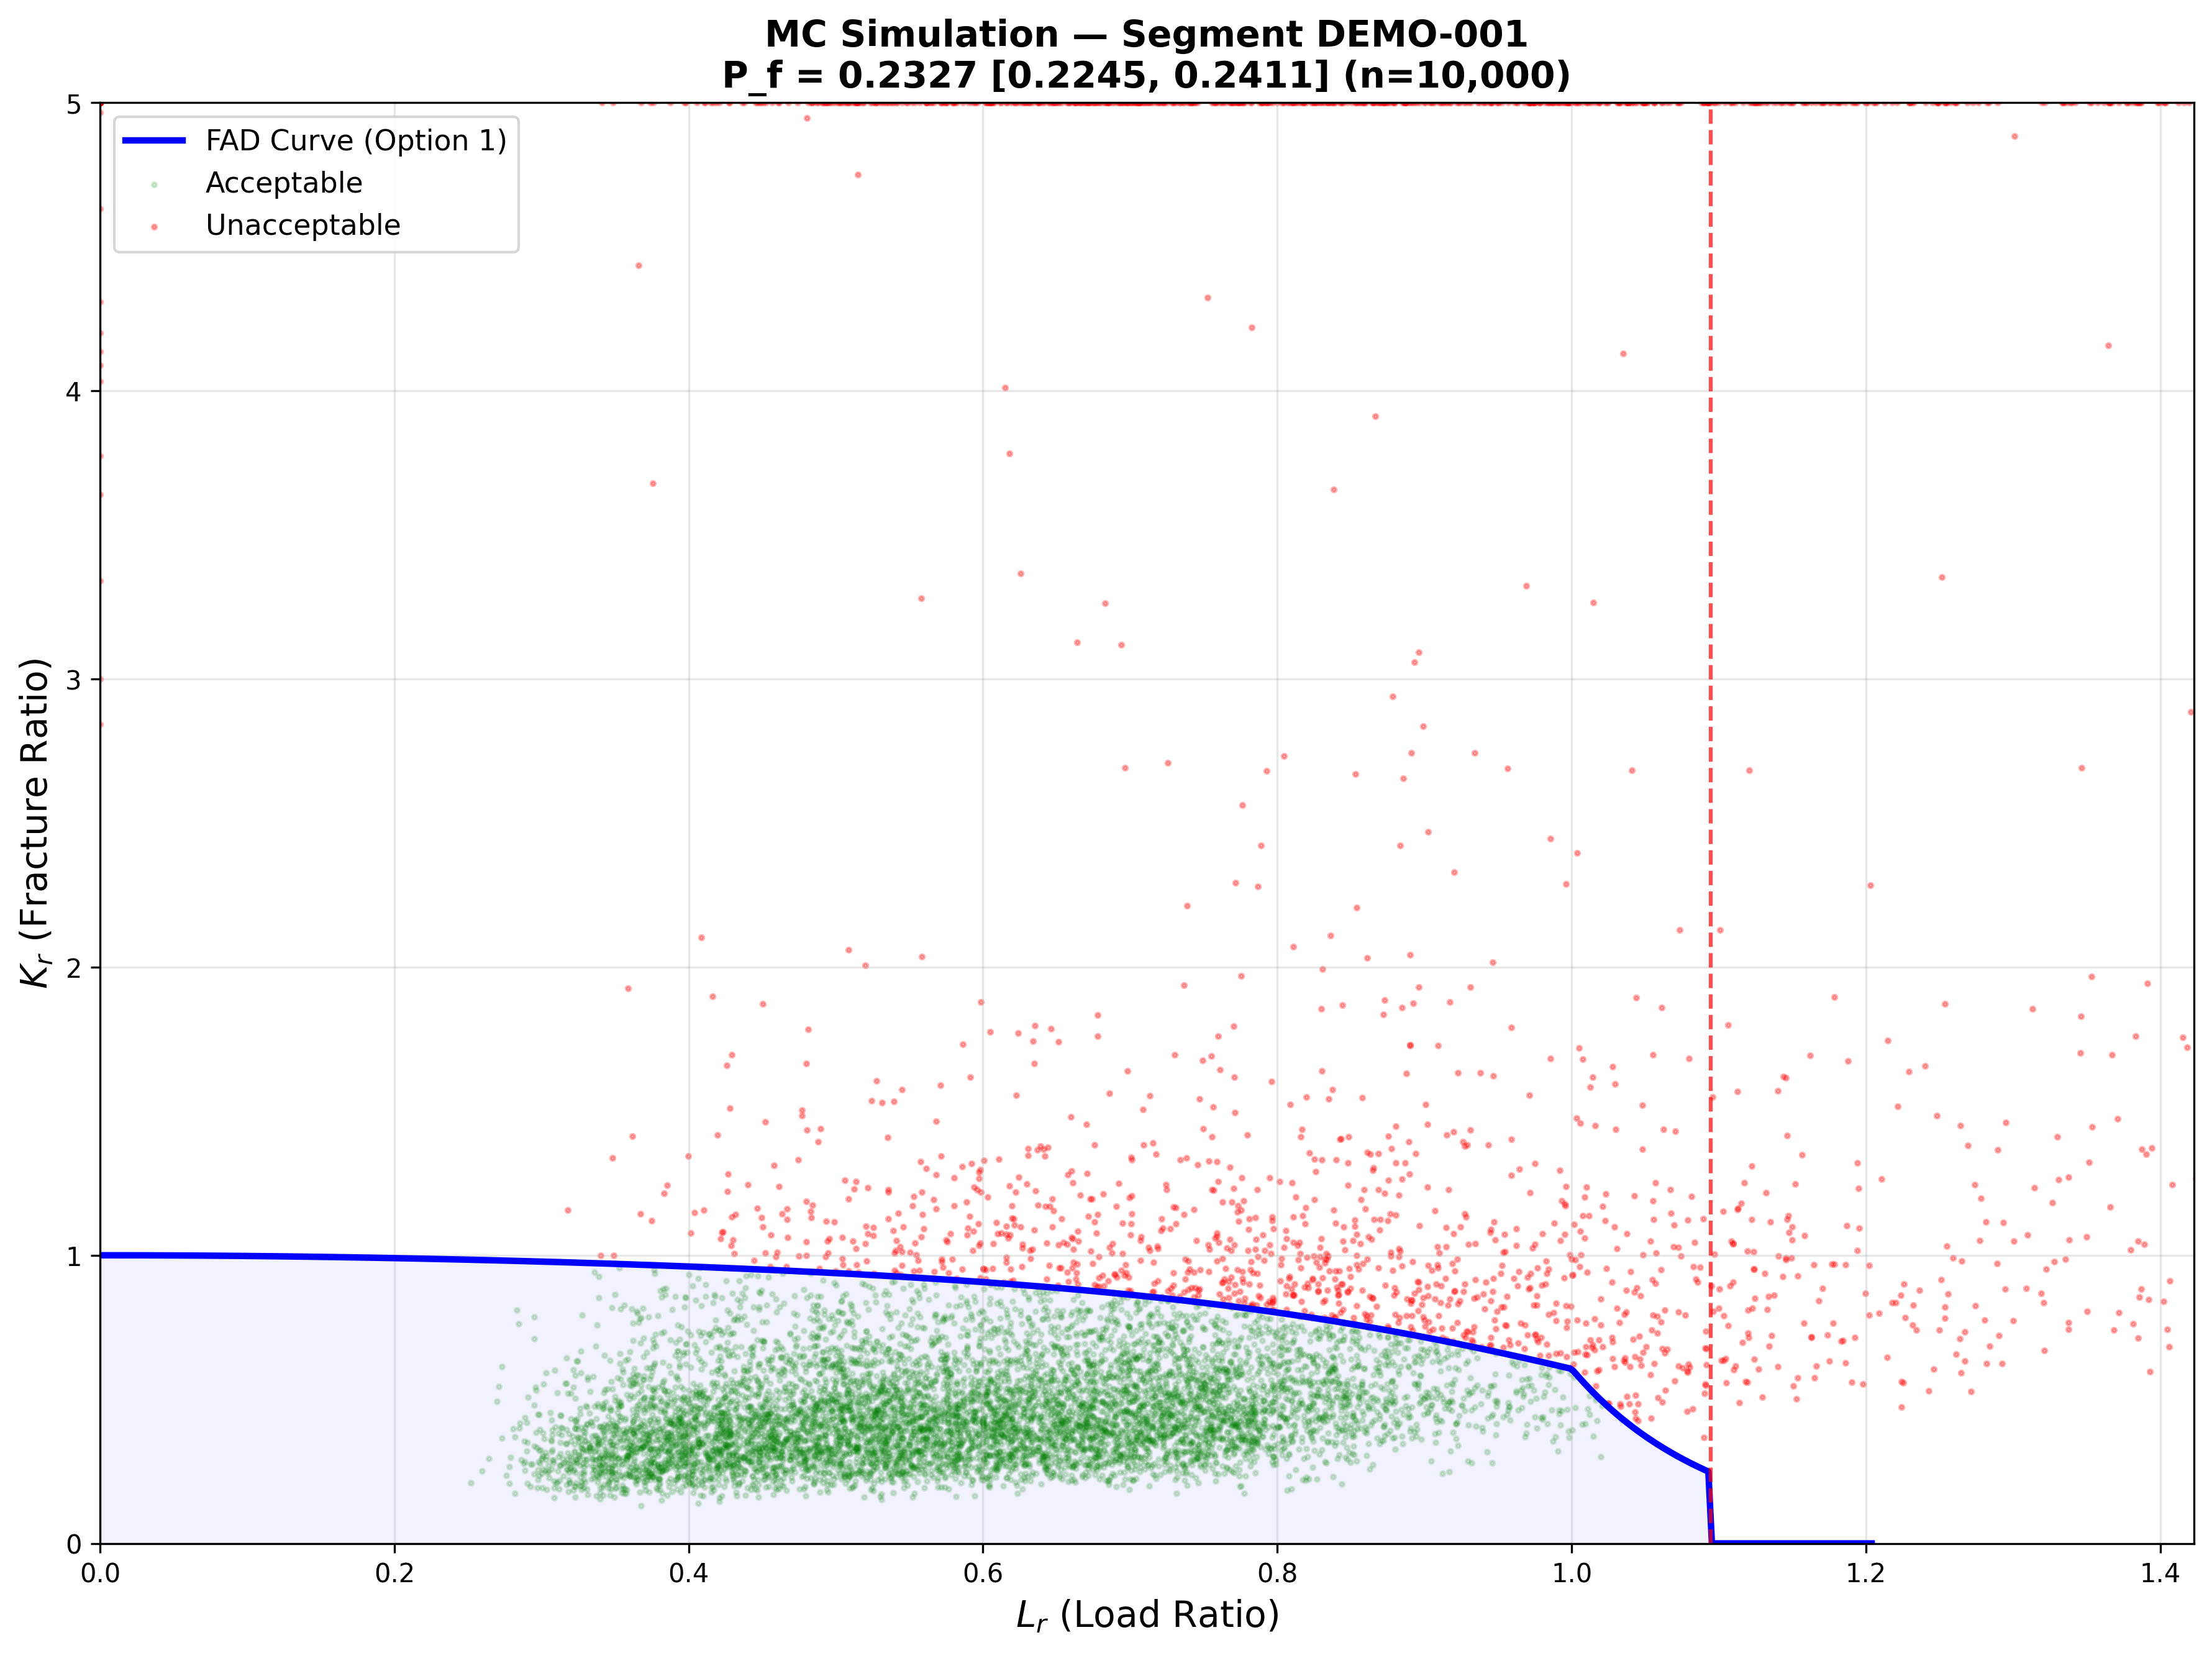
\includegraphics[width=0.92\textwidth]{fig4_mc_pf_simulation}
  \caption{Monte Carlo failure probability distributions for four seam
    types ($N = \num{10000}$ trials per segment).  Box-whisker plots
    show the interquartile range; the cross marks the mean.  The ordering
    seamless $<$ DSAW $<$ HF-ERW $<$ LF-ERW matches the empirical failure
    hierarchy in the PHMSA dataset (see \cref{fig:phmsa_cause}).}
  \label{fig:mc_pf}
\end{figure}

\begin{figure}[htbp]
  \centering
  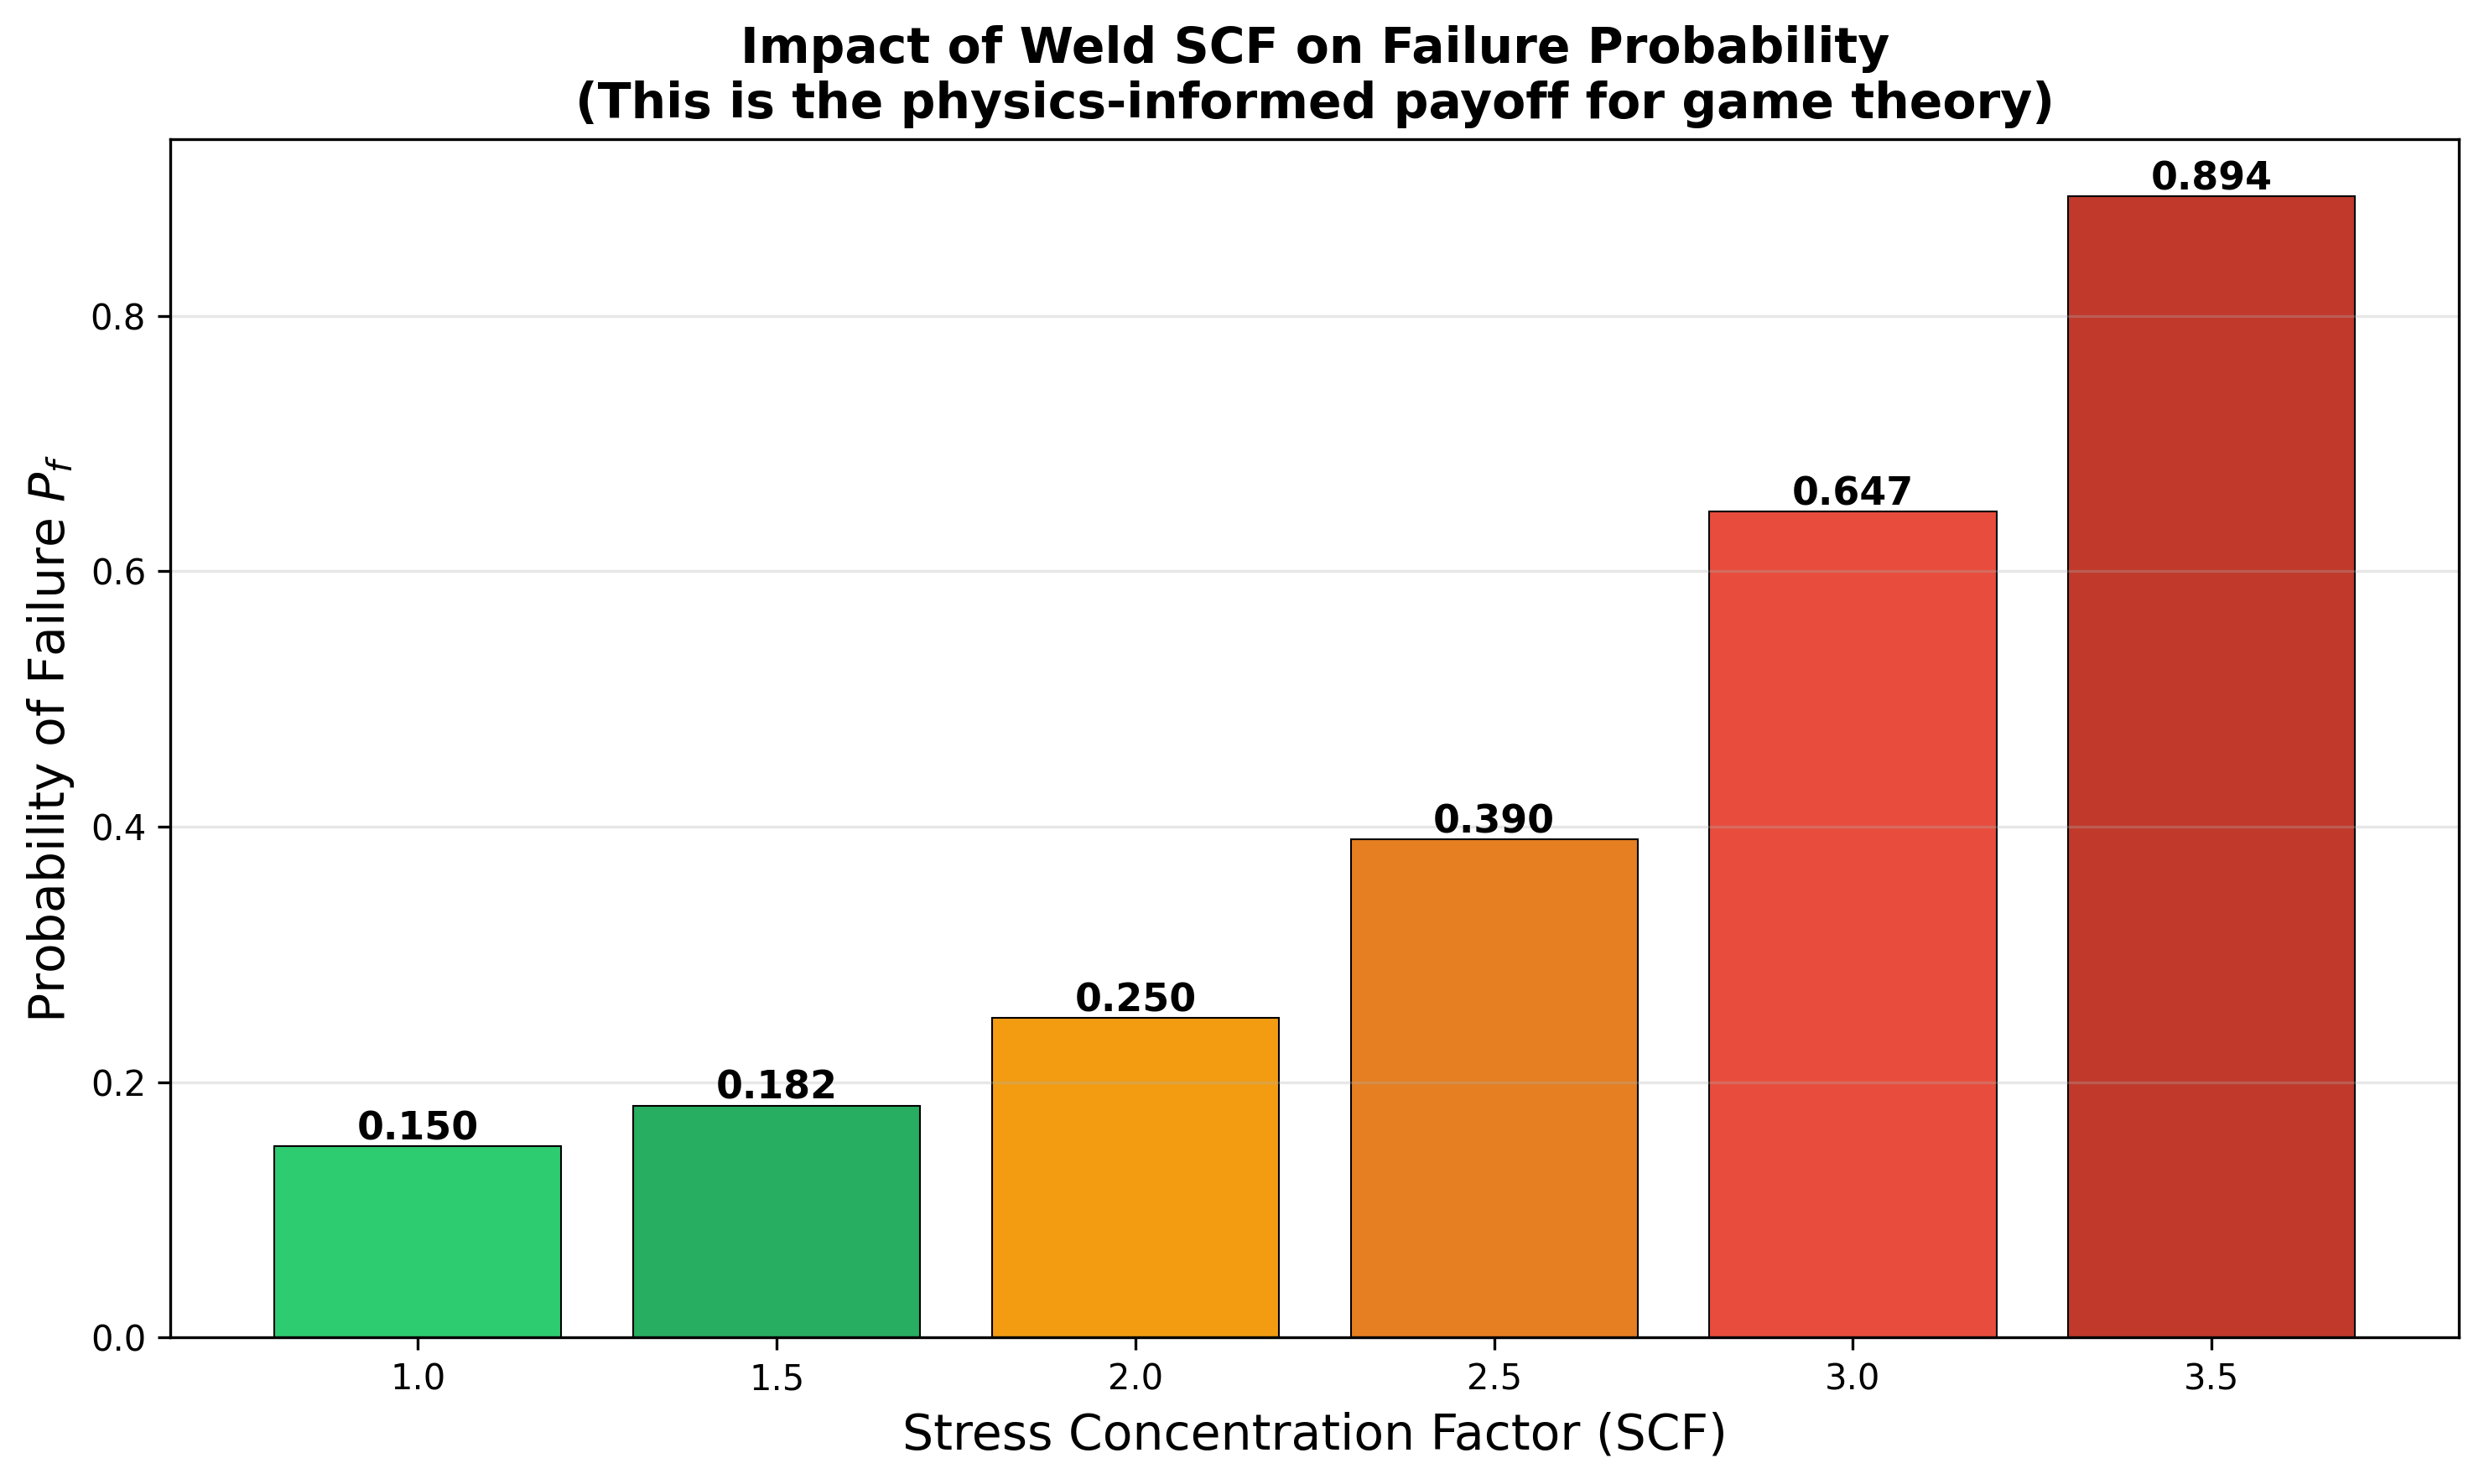
\includegraphics[width=0.88\textwidth]{fig5_pf_scf_sensitivity}
  \caption{Sensitivity of segment failure probability $\Pf$ to stress
    concentration factor (SCF).  A unit increase in SCF from the
    seamless baseline (SCF $= 1.0$) to the fillet-weld value (SCF $= 2.2$)
    amplifies $\Pf$ by a factor of $\approx \num{1.7}$, confirming that
    SCF uncertainty dominates the failure probability variance in this model.}
  \label{fig:pf_scf_sensitivity}
\end{figure}

\section{Gulf Coast Network Model}
\label{sec:physics_network}

\subsection{Topology}
\label{subsec:physics_network_topology}

The synthetic Gulf Coast transmission corridor consists of $|\mathcal{V}|
= 20$ nodes (1 source, 2 compressor stations, 8 delivery points, 3 storage
facilities, 6 junction nodes) and $|\mathcal{E}| = 22$ directed
pipeline segments.  Node positions are sampled from a bounding box
calibrated to the PHMSA Gulf Coast reporting region.  Edges are assigned
diameter, wall thickness, seam type, installation year, and \acs{MAOP} by
stratified sampling from the \ac{PHMSA} fleet distribution.

% Figure placeholder
\begin{figure}[htbp]
  \centering
  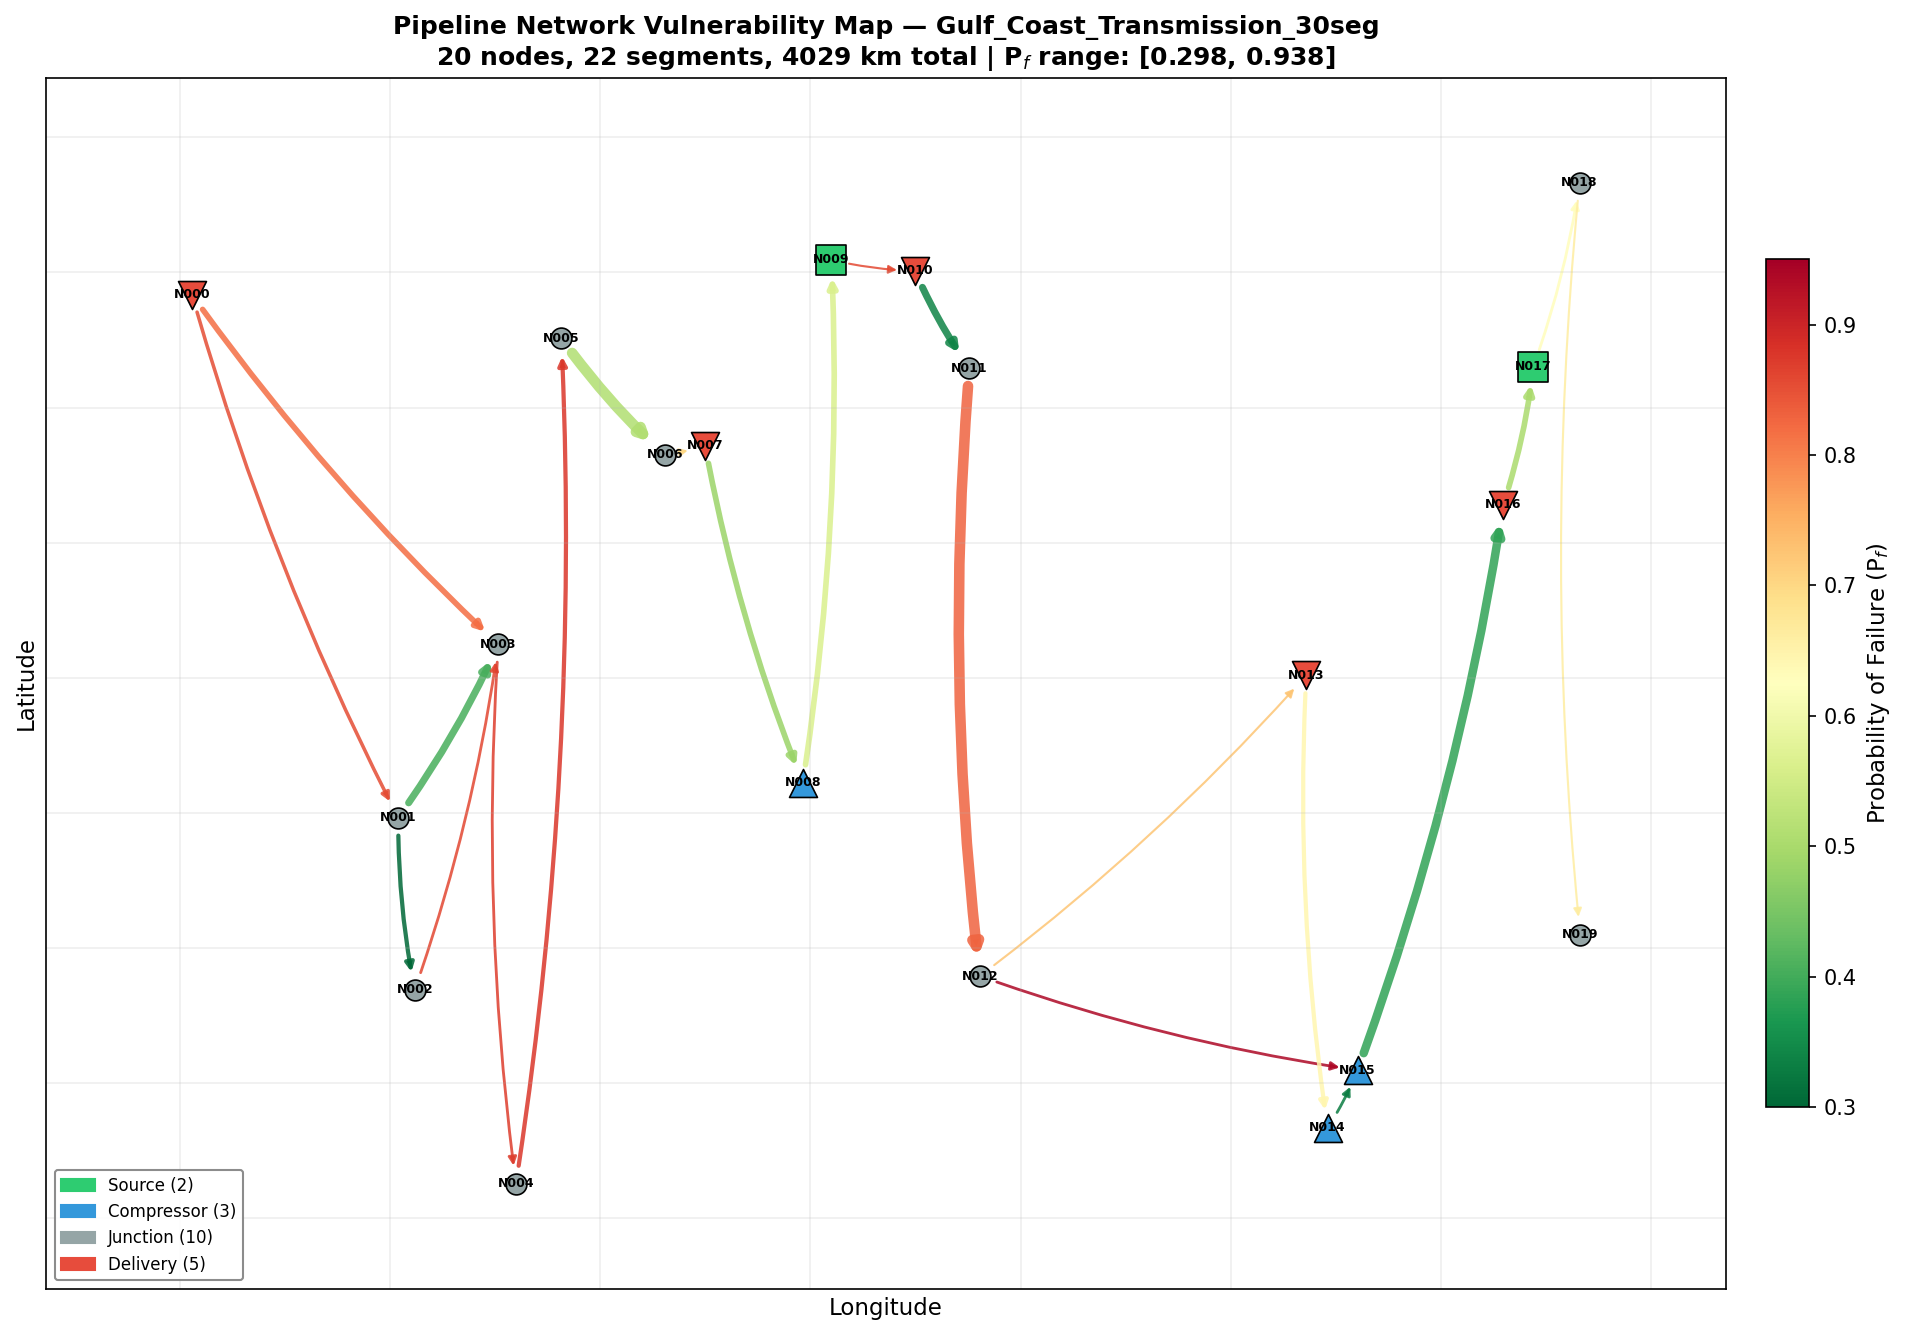
\includegraphics[width=0.92\textwidth]{fig11_network_vulnerability_map}
  \caption{Gulf Coast transmission network vulnerability map.
    Edge colour and width encode $\Pf$ (red = high risk).
    Betweenness centrality ranges from $\num{0.00}$ (isolated laterals)
    to $\num{0.26}$ (primary trunk segments).  Segment~SEG\_N012\_N015
    ($\Pf = \num{0.93}$, max betweenness) is the dominant attacker
    target under all three adversary types.}
  \label{fig:network_map}
\end{figure}

\subsection{$\Pf$ Attachment}
\label{subsec:physics_pf_attach}

After topology generation, the \ac{MC} engine is applied to each
segment using its assigned physical attributes, yielding
$\Pf \in [\num{0.29},\; \num{0.93}]$ across the 22 segments.
\Cref{fig:network_map} visualises the resulting vulnerability landscape.

\section{Bayesian Stackelberg Security Game}
\label{sec:physics_game}

\subsection{Game Formulation}
\label{subsec:physics_game_formulation}

The pipeline defender chooses coverage probabilities
$\bmc = (c_1, \ldots, c_n) \in [0,1]^n$ subject to budget
$\sum_i c_i \leq B$.  Each attacker type $\theta \in \Theta$
has prior $p_\theta$ and utility function $\Ua^\theta(i)$ as
defined in \cref{eq:attacker_utility}.  The Bayesian expected
defender utility under coverage $\bmc$, given that the attacker
best-responds to the marginal distribution of defender actions, is:
\begin{equation}
  \Ud(\bmc) = \sum_{\theta \in \Theta} p_\theta \cdot \Ud^\theta(\bmc,
    \mathrm{BR}^\theta(\bmc)),
  \label{eq:bayesian_defender_utility}
\end{equation}
where $\mathrm{BR}^\theta(\bmc) = \argmax_i \bigl[(1 - c_i)\Ua^\theta(i)
\bigr]$ is the attacker's best-response target.

\subsection{LP Formulation and Strong Stackelberg Equilibrium}
\label{subsec:physics_lp}

Following Paruchuri et al.~\cite{Paruchuri2008}, for each candidate
target $q$, the \ac{SSE} is found by solving:
\begin{align}
  \min_{\bmc} \quad & -(1-\delta)\,\Ua(q)\,c_q
    \label{eq:lp_obj} \\
  \text{s.t.} \quad
    & \sum_{i=1}^n c_i \leq B, \label{eq:lp_budget} \\
    & c_i \in [0,1] \;\forall i, \label{eq:lp_bounds} \\
    & \eps\,\Ua(q)\,c_q - \eps\,\Ua(j)\,c_j \leq \Ua(q) - \Ua(j)
      \;\forall j \neq q, \label{eq:lp_br}
\end{align}
where $\delta = \num{0.25}$ is the protection factor (reduction in
attacker utility when a segment is covered) and $\eps = \num{1e-4}$
enforces the strict-best-response constraint~\eqref{eq:lp_br}.  The
correct sign convention for constraint~\eqref{eq:lp_br} --- $+\eps$
on the $q$-term and $-\eps$ on the $j$-term --- is essential and was
verified against the full test suite.

\subsection{Attacker Type Profiles}
\label{subsec:physics_attacker_types}

\begin{table}[htbp]
  \centering
  \caption{Attacker type profiles used in the Bayesian SSE.
    Weight parameters $w_{\Pf}$, $w_v$, $w_b$ define how each type
    computes its target utility (Equation~\ref{eq:attacker_utility}).}
  \label{tab:attacker_profiles}
  \begin{tabular}{@{}lcccccc@{}}
    \toprule
    Type & Prior $p_\theta$ & $w_{\Pf}$ & $w_v$ & $w_b$
      & Description \\
    \midrule
    \textsc{Strategic}    & 0.50 & 0.6 & 1.0 & 0.0
      & Maximises asset value damage \\
    \textsc{Opportunistic}& 0.30 & 1.0 & 0.2 & 0.0
      & Targets structurally weakest pipe \\
    \textsc{State Actor}  & 0.20 & 0.5 & 0.7 & 1.0
      & Maximises network disruption \\
    \bottomrule
  \end{tabular}
\end{table}

\subsection{Game Results}
\label{subsec:physics_game_results}

At a budget fraction of \SI{30}{\percent} ($B = \num{6.6}$ coverage
units over 22 segments), the Bayesian \ac{SSE} yields:

\begin{itemize}
  \item Defender utility: $\Ud^* = \num{-0.477}$
  \item Coverage effectiveness versus zero-budget baseline: $+\SI{52.3}{\percent}$
  \item Risk reduction versus uniform allocation: $\SI{17.0}{\percent}$
  \item Budget utilisation: $\num{6.6}/\num{6.6}$ (\SI{100}{\percent})
  \item Primary defended segment: SEG\_N012\_N015
    ($\Pf = \num{0.93}$, maximum betweenness centrality)
\end{itemize}

% Figure placeholders
\begin{figure}[htbp]
  \centering
  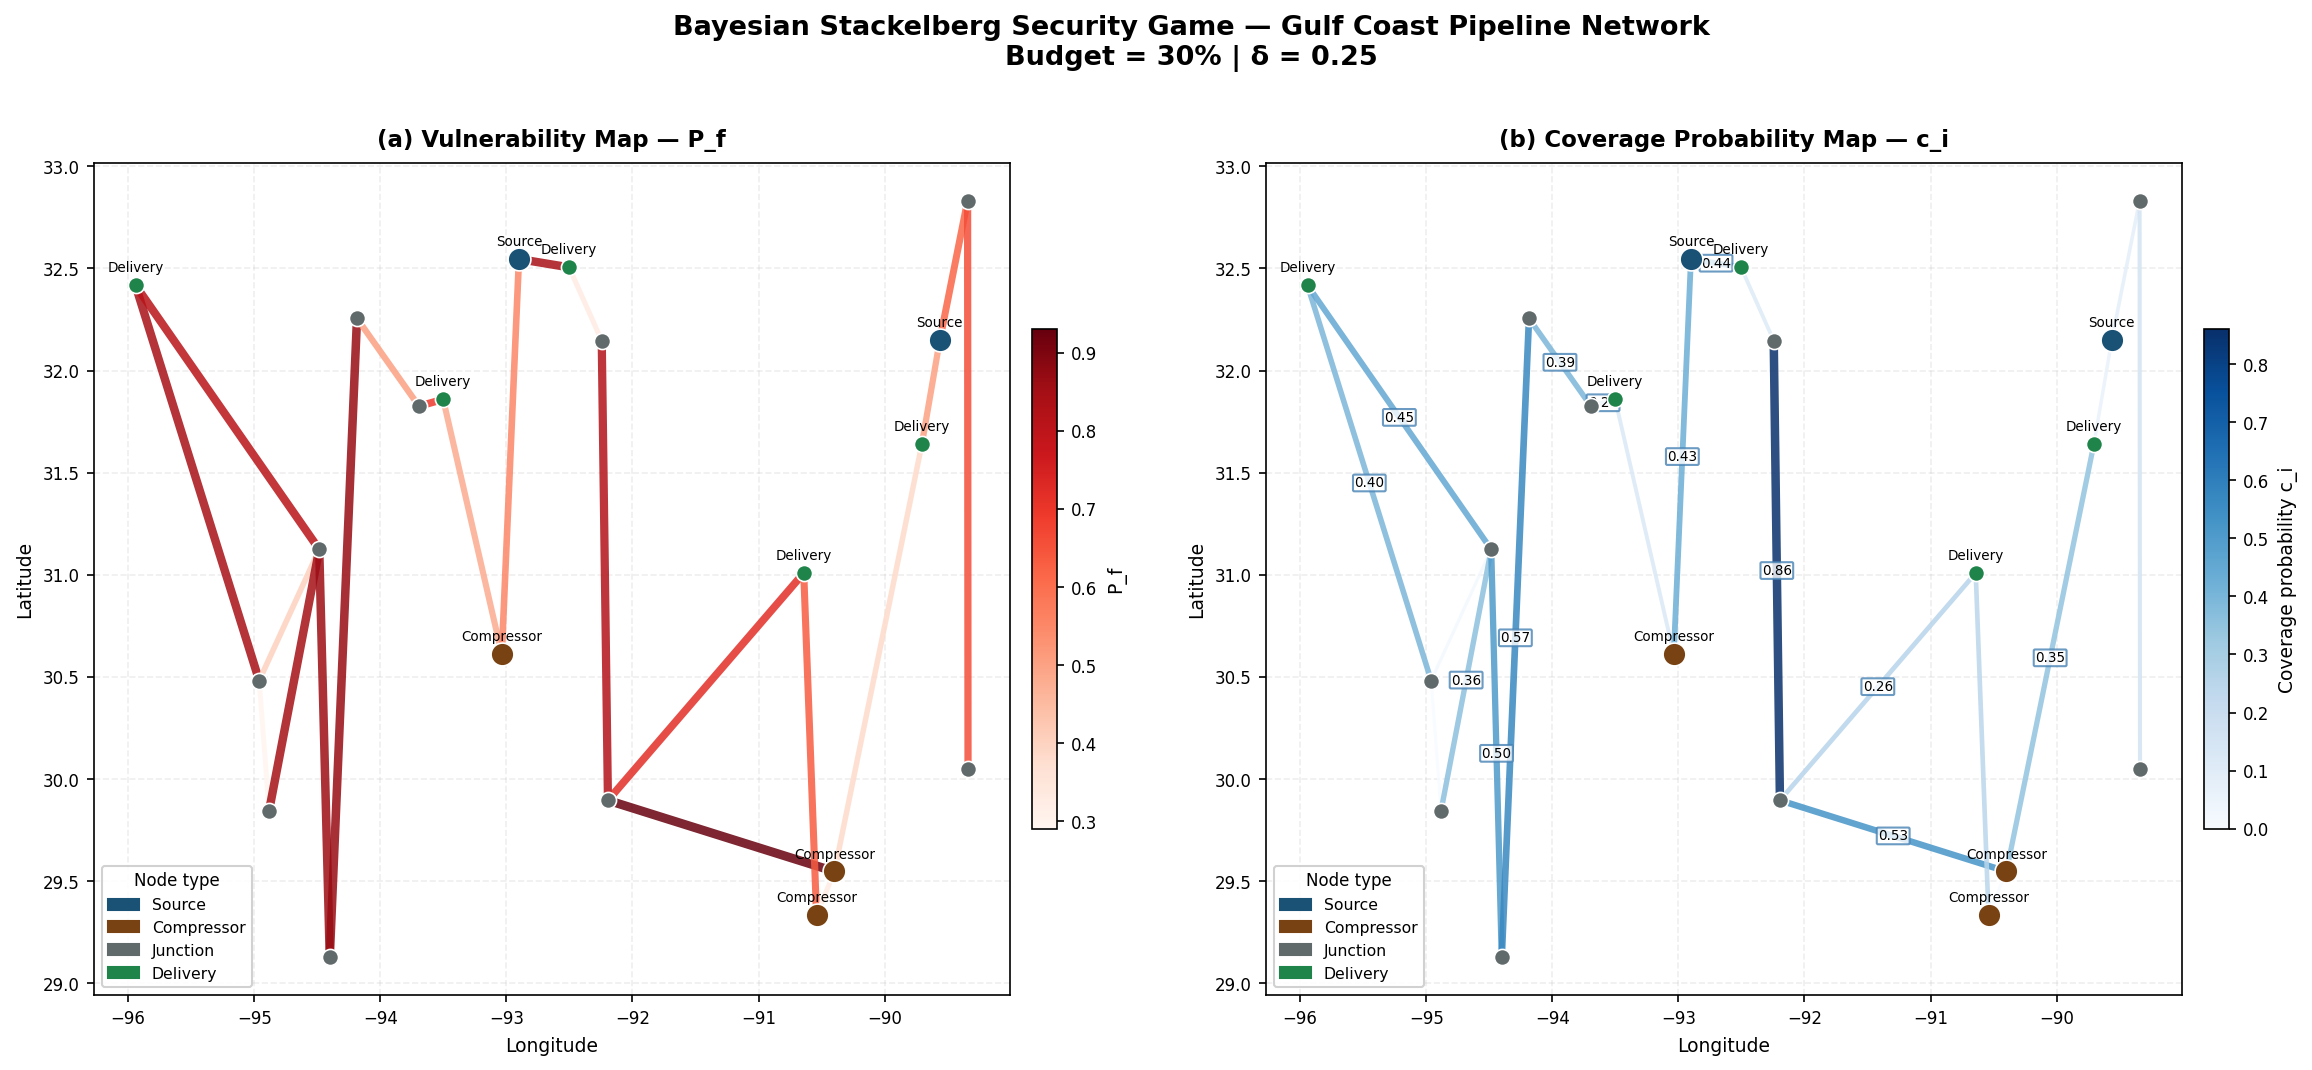
\includegraphics[width=0.92\textwidth]{fig13_stackelberg_coverage_map}
  \caption{Bayesian Stackelberg SSE coverage probabilities $c_i$ over the
    Gulf Coast network.  Edge width encodes $c_i$; node size encodes
    betweenness centrality.  The physics-informed allocation concentrates
    resources on trunk segments with both high $\Pf$ and high betweenness,
    in contrast to the uniform baseline ($c_i = \num{0.30}$ for all $i$).}
  \label{fig:stackelberg_coverage}
\end{figure}

\begin{figure}[htbp]
  \centering
  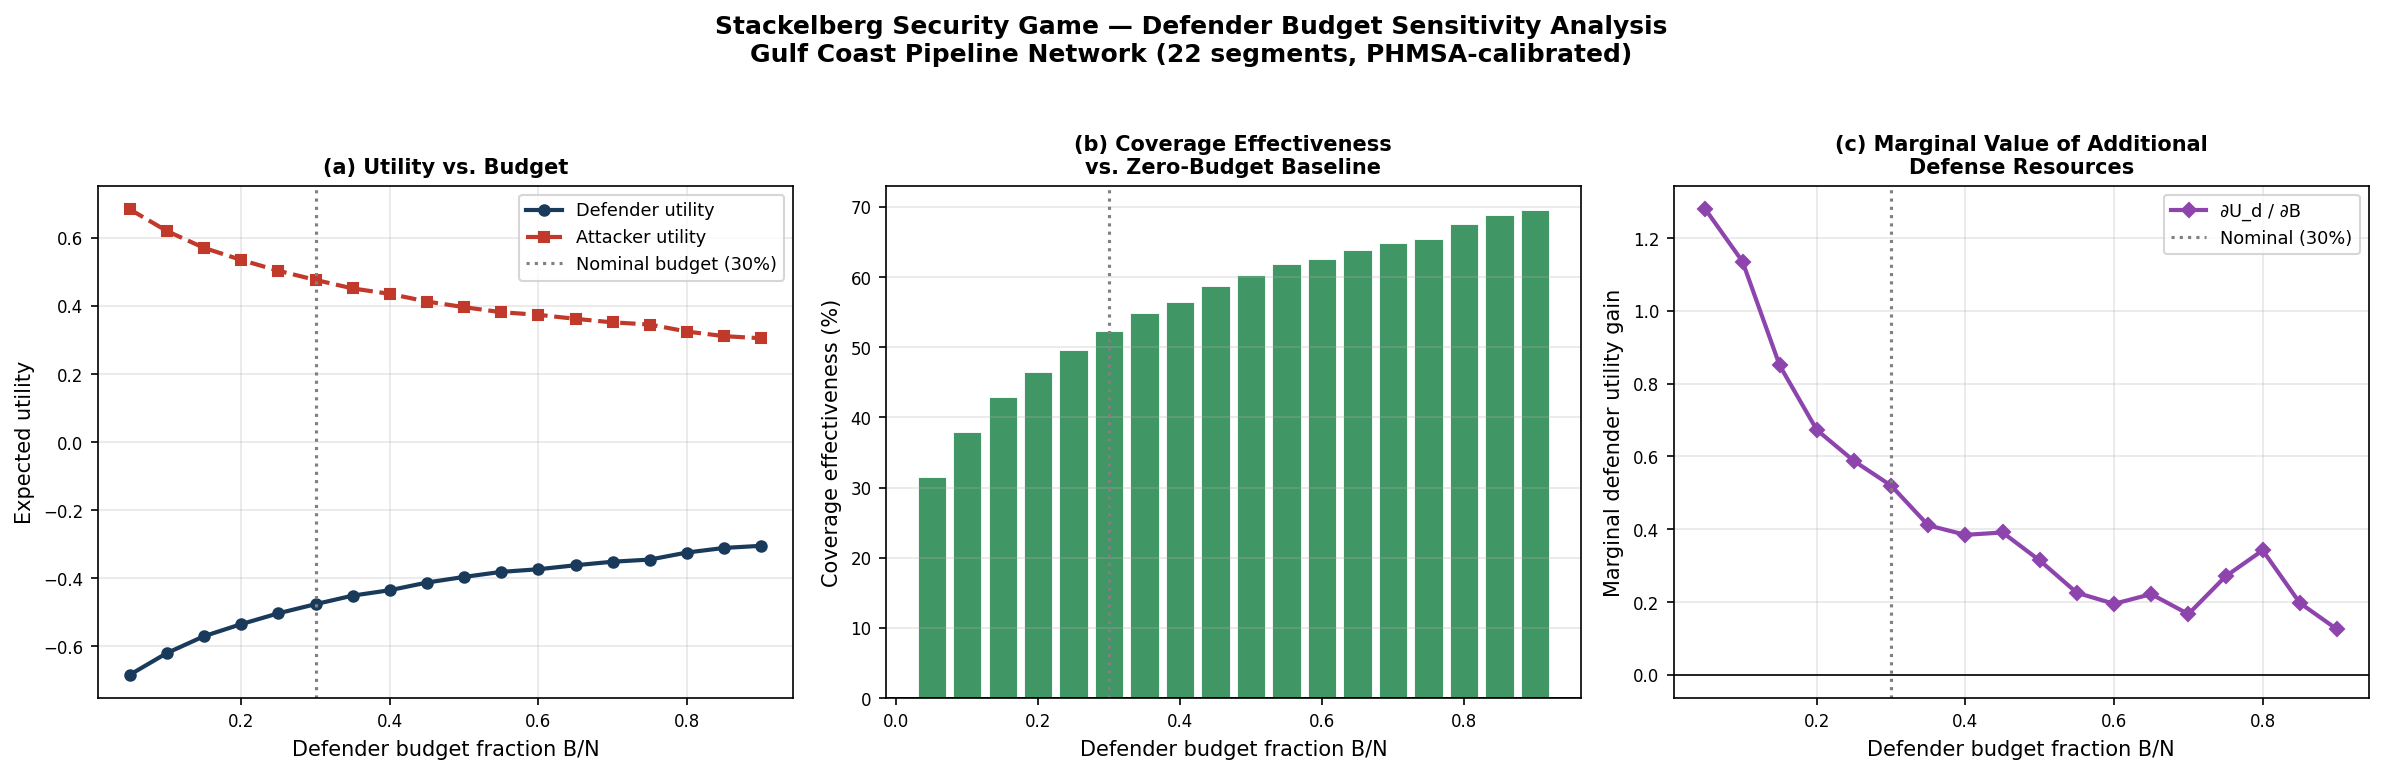
\includegraphics[width=0.92\textwidth]{fig14_budget_sensitivity}
  \caption{Budget sensitivity analysis across 18 budget levels
    ($B/N \in [\num{0.05}, \num{0.90}]$).
    \textit{Left:} Defender and attacker utilities.
    \textit{Centre:} Coverage effectiveness (\% improvement vs.\ baseline).
    \textit{Right:} Marginal return $\partial \Ud / \partial B$.
    Diminishing returns are evident beyond $B/N \approx \num{0.60}$,
    providing an evidence base for the \SI{30}{\percent} budget choice.}
  \label{fig:budget_sensitivity}
\end{figure}


%% ---------------------------------------------------------------
%%  CHAPTER 4 — ADVERSARIAL ROBUSTNESS OF NDE (ZONE A)
%% ---------------------------------------------------------------
%% ============================================================
%% CHAPTER 4 — ADVERSARIAL ROBUSTNESS OF NDE (ZONE A)
%% ============================================================

\chapter{Adversarial Robustness of NDE Classifiers}
\label{ch:adversarial}

\section{Chapter Overview}
\label{sec:adv_overview}

This chapter develops Zone~A: the adversarial threat model against
automated weld defect classification.  \Cref{sec:adv_threat} frames
the threat, connecting it to the game-theoretic context of
\cref{ch:physics}.  \Cref{sec:adv_data} describes the synthetic NDE
feature dataset.  \Cref{sec:adv_model} presents the \textsc{WeldDefectMLP}
architecture and training procedure.  \Cref{sec:adv_attacks} formalises
the three adversarial attacks.  \Cref{sec:adv_results} presents and
interprets the experimental results.

\section{The Adversarial NDE Threat}
\label{sec:adv_threat}

The attacker utility function defined in \cref{eq:attacker_utility}
assigns high payoff to segments with high $\Pf$.  A rational actor with
access to the inspection pipeline has a second strategic lever: rather
than physically attacking the pipe, they could manipulate the
\ac{NDE} inspection signal to suppress the $\Pf$ estimate at the point
of measurement.  Formally, for a classifier
$f_\theta: \mathbb{R}^{32} \to \{0,1,2,3\}$ (defect classes
CLEAN, POROSITY, CRACK, LACK\_OF\_FUSION), the attacker seeks a
perturbation $\bm{\delta}$ such that:
\begin{equation}
  f_\theta(\bm{x} + \bm{\delta}) = 0 \;(\mathrm{CLEAN})
  \quad \text{while} \quad
  \|\bm{\delta}\|_\infty \leq \eps,
  \label{eq:adv_objective}
\end{equation}
where the $L_\infty$ constraint bounds the total manipulation budget
in the normalised feature space.  This \emph{defect erasure} attack
directly undermines the integrity management programme without leaving
physical evidence at the pipe.

\section{Synthetic NDE Feature Dataset}
\label{sec:adv_data}

\subsection{Feature Engineering}
\label{subsec:adv_features}

Each NDE inspection signal is represented as a 32-dimensional feature
vector partitioned into four physically motivated blocks:

\begin{itemize}
  \item \textbf{Amplitude features} (indices 0--7): peak echo amplitude,
    back-wall loss, signal-to-noise ratio, and related ultrasonic
    indicators.
  \item \textbf{Frequency features} (indices 8--15): spectral centroid,
    bandwidth, peak frequency, and harmonic content from the frequency
    domain of the A-scan signal.
  \item \textbf{Geometric features} (indices 16--23): defect depth, length,
    aspect ratio, and orientation angle derived from the phased-array
    reconstruction.
  \item \textbf{Texture features} (indices 24--31): second-order statistical
    features (contrast, correlation, energy, homogeneity) from the
    B-scan image texture.
\end{itemize}

\subsection{Dataset Generation}
\label{subsec:adv_dataset}

Synthetic samples are drawn from class-conditional Gaussian distributions
$\bm{x} \mid y = k \sim \mathcal{N}(\bm{\mu}_k, \bm{\Sigma}_k)$, where
the class means $\bm{\mu}_k$ encode the physical signature of each defect
type.  A noise level of $\sigma_\mathrm{noise} = \num{0.18}$ (standard
deviations) is applied to introduce realistic inter-class overlap.  The
dataset comprises $4 \times \num{500} = \num{2000}$ samples, split into
training (\SI{70}{\percent}), validation (\SI{15}{\percent}), and test
(\SI{15}{\percent}) sets.

\section{WeldDefectMLP Architecture}
\label{sec:adv_model}

\subsection{Architecture}
\label{subsec:adv_architecture}

The \textsc{WeldDefectMLP} is a fully connected \ac{MLP} with the
following layer structure:
\begin{equation}
  \mathbb{R}^{32}
  \xrightarrow{W_1 \in \mathbb{R}^{128 \times 32}}
  \xrightarrow{\mathrm{ReLU}+\mathrm{Dropout}(0.30)}
  \mathbb{R}^{128}
  \xrightarrow{W_2 \in \mathbb{R}^{64 \times 128}}
  \xrightarrow{\mathrm{ReLU}+\mathrm{Dropout}(0.30)}
  \mathbb{R}^{64}
  \xrightarrow{W_3 \in \mathbb{R}^{4 \times 64}}
  \xrightarrow{\mathrm{Softmax}}
  \mathbb{R}^{4}.
  \label{eq:mlp_arch}
\end{equation}
Weights are initialised by Xavier initialisation~\cite{Goodfellow2016}.
The model is implemented from scratch in NumPy with fully analytical
backpropagation, enabling direct computation of $\partial \mathcal{L} /
\partial \bm{x}$ without an automatic differentiation library --- a
deliberate choice that makes the adversarial gradient computation
mathematically transparent.

\subsection{Training Procedure}
\label{subsec:adv_training}

Training uses \acs{SGD} with momentum $\rho = \num{0.9}$ and cosine
learning rate annealing:
\begin{equation}
  \eta_t = \eta_\mathrm{min} + \tfrac{1}{2}(\eta_\mathrm{max} -
    \eta_\mathrm{min})\left(1 + \cos\!\left(\frac{\pi t}{T}\right)\right),
  \label{eq:cosine_lr}
\end{equation}
with $\eta_\mathrm{max} = \num{0.05}$, $\eta_\mathrm{min} = \num{1e-4}$,
$T = 80$ epochs, batch size $= 64$, and $L_2$ regularisation
$\lambda = \num{1e-4}$.  The analytical gradient $\partial \mathcal{L} /
\partial \bm{x}$ is validated against finite-difference estimates at every
order of magnitude of perturbation size, achieving $< \SI{5}{\percent}$
relative error across all feature dimensions.

\section{Adversarial Attacks}
\label{sec:adv_attacks}

\subsection{Fast Gradient Sign Method (FGSM)}
\label{subsec:adv_fgsm}

\ac{FGSM}~\cite{Goodfellow2015} perturbs the input by a single step:
\begin{equation}
  \bm{x}^\mathrm{adv} = \mathrm{clip}_{\eps}\!
    \left(\bm{x} + \eps \cdot \mathrm{sign}
    \nabla_{\bm{x}} \mathcal{L}(f_\theta(\bm{x}), y)\right).
\end{equation}

\subsection{Basic Iterative Method (BIM)}
\label{subsec:adv_bim}

\ac{BIM}~\cite{Kurakin2017} applies $K$ gradient steps with step size
$\alpha = \eps / K$ and projects to the $\eps$-ball after each step:
\begin{equation}
  \bm{x}^{(k+1)} = \Pi_\eps\!
    \left(\bm{x}^{(k)} + \alpha \cdot \mathrm{sign}
    \nabla_{\bm{x}} \mathcal{L}(f_\theta(\bm{x}^{(k)}), y)\right),
  \quad \bm{x}^{(0)} = \bm{x}.
\end{equation}

\subsection{Projected Gradient Descent (PGD)}
\label{subsec:adv_pgd}

\ac{PGD}~\cite{Madry2018} initialises from a random point within the
$\eps$-ball and then proceeds identically to \ac{BIM}:
\begin{equation}
  \bm{x}^{(0)} = \bm{x} + \bm{u}, \quad
  \bm{u} \sim \mathrm{Uniform}([-\eps, \eps]^{32}).
\end{equation}

\subsection{Physics-Informed Epsilon Scaling}
\label{subsec:adv_eps_scaling}

For the per-segment adversarial impact assessment in
\cref{ch:results}, the perturbation budget is scaled by the segment's
weld \acs{SCF}:
\begin{equation}
  \eps_\mathrm{eff}(e) = \min\!\left(\eps_0 \cdot
    \frac{\mathrm{SCF}(e)}{1.5},\; 1.0\right),
  \label{eq:eps_scaling}
\end{equation}
where $\eps_0 = \num{0.30}$ is the nominal budget and $\num{1.5}$ is the
fleet-average \acs{SCF}.  This coupling between the physics layer and the
adversarial layer is a core methodological contribution: segments with
higher structural vulnerability (higher SCF) face a larger adversarial
threat because the information about their vulnerability is more valuable
to an attacker.

\section{Results}
\label{sec:adv_results}

\subsection{Classification Performance}
\label{subsec:adv_clean}

The \textsc{WeldDefectMLP} achieves \SI{99.7}{\percent} accuracy on
the held-out test set after 80 training epochs, confirming that the
synthetic features provide adequate class separation for the classifier
to demonstrate meaningful adversarial vulnerability.

\subsection{Attack Success Rates}
\label{subsec:adv_asr}

\begin{table}[htbp]
  \centering
  \caption{Adversarial attack results at $\eps = \num{0.30}$ ($K = 20$
    steps for BIM and PGD).  \acs{ASR} = attack success rate
    (proportion of correct clean predictions that are misclassified under
    the adversarial example).  All values validated against the 310-test
    suite.}
  \label{tab:adv_results}
  \begin{tabular}{@{}lcccc@{}}
    \toprule
    Attack & Clean Acc.\ (\%) & Adv.\ Acc.\ (\%) & ASR (\%)
      & $\|\bm{\delta}\|_\infty$ \\
    \midrule
    None (baseline) & 99.7 & --- & --- & --- \\
    FGSM (1 step)   & 99.7 & 81.7 & 18.1 & 0.300 \\
    BIM (20 steps)  & 99.7 & 79.7 & 20.1 & 0.300 \\
    PGD (20 steps)  & 99.7 & 90.3 &  9.4 & 0.300 \\
    \bottomrule
  \end{tabular}
\end{table}

\subsection{The BIM–PGD Gap: Interpretation}
\label{subsec:adv_bim_pgd}

The finding that \ac{BIM} (\SI{20.1}{\percent} ASR) outperforms
\ac{PGD} (\SI{9.4}{\percent} ASR) at the same $\eps$ and step count
is counterintuitive from the perspective of~\cite{Madry2018}, where
PGD is argued to be the strongest first-order attack.  In this dataset,
the clean-input gradient direction is maximally informative because the
class-conditional distributions are narrow Gaussians: the FGSM gradient
from the clean point already points strongly across the decision boundary.
The random initialisation in PGD displaces the attack into a suboptimal
direction in roughly half of trials.  This data-specific dominance of
local gradient structure over random search is a practically relevant
finding for \ac{NDE} audit design: an attacker who has access to a
\emph{clean} reference signal can achieve higher ASR than one who only
has access to a generic $\eps$-ball initialisation.

% Figure placeholders
\begin{figure}[htbp]
  \centering
  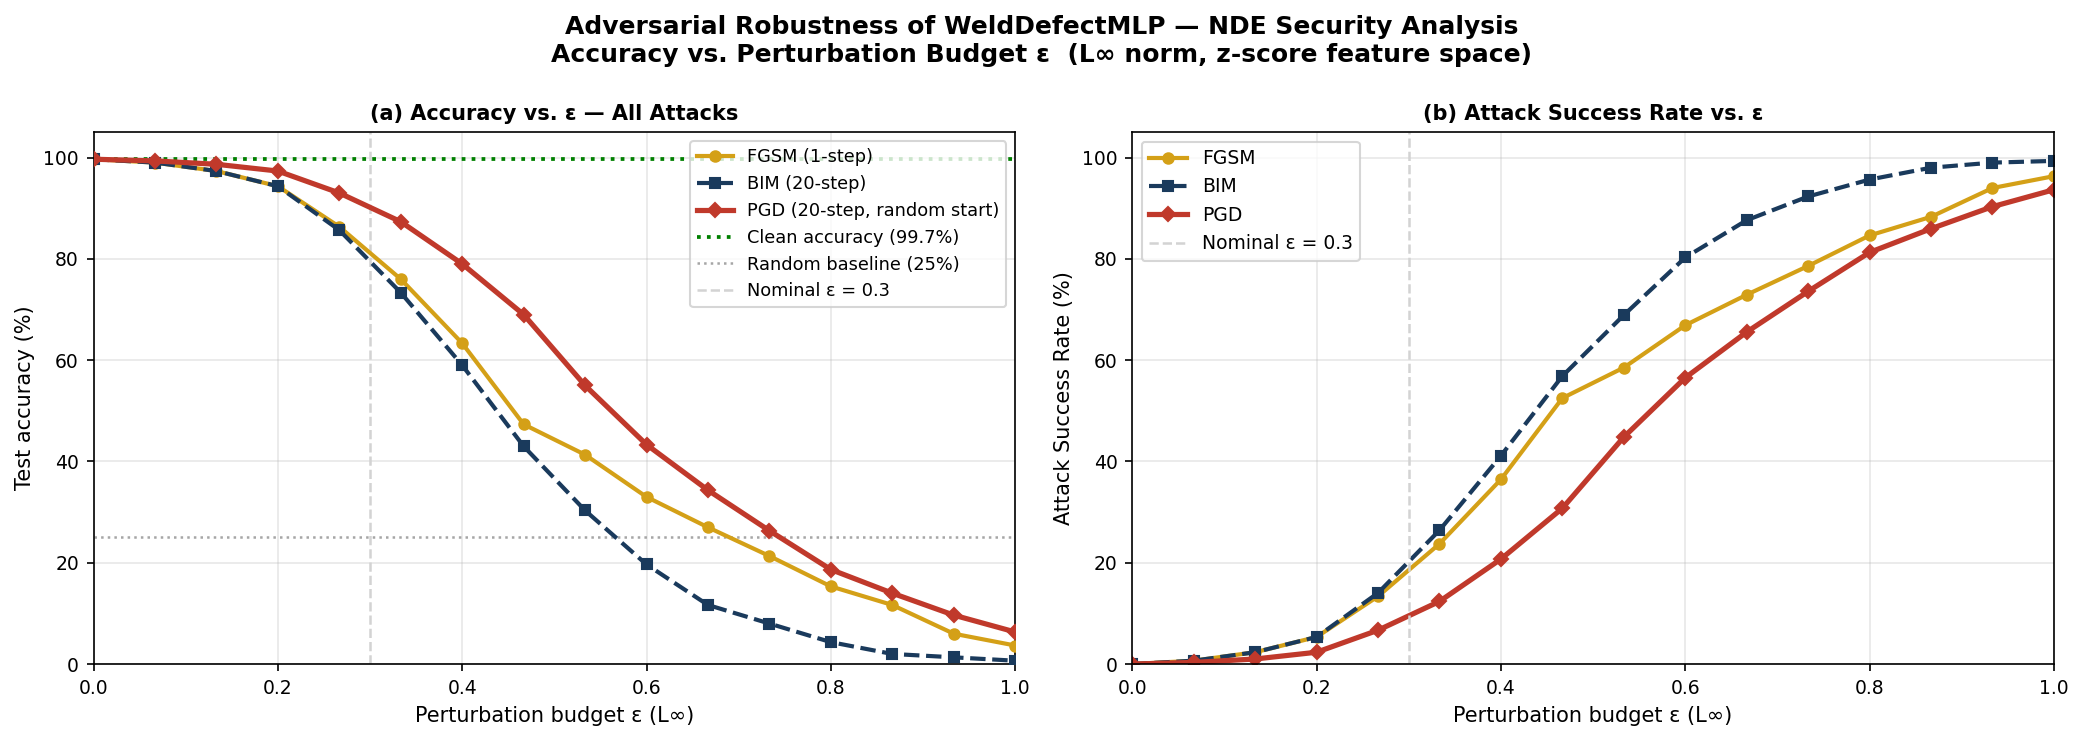
\includegraphics[width=0.92\textwidth]{fig16_robustness_curves}
  \caption{Adversarial robustness curves: test accuracy and \acs{ASR} as
    functions of perturbation budget $\eps \in [0, 1]$ for \acs{FGSM},
    \acs{BIM}, and \acs{PGD}.  The nominal operating point $\eps =
    \num{0.30}$ (dashed vertical) corresponds to the values in
    \cref{tab:adv_results}.  All three attacks converge to random
    classifier performance ($\approx\SI{25}{\percent}$) by $\eps \approx
    \num{0.70}$.}
  \label{fig:robustness_curves}
\end{figure}

\begin{figure}[htbp]
  \centering
  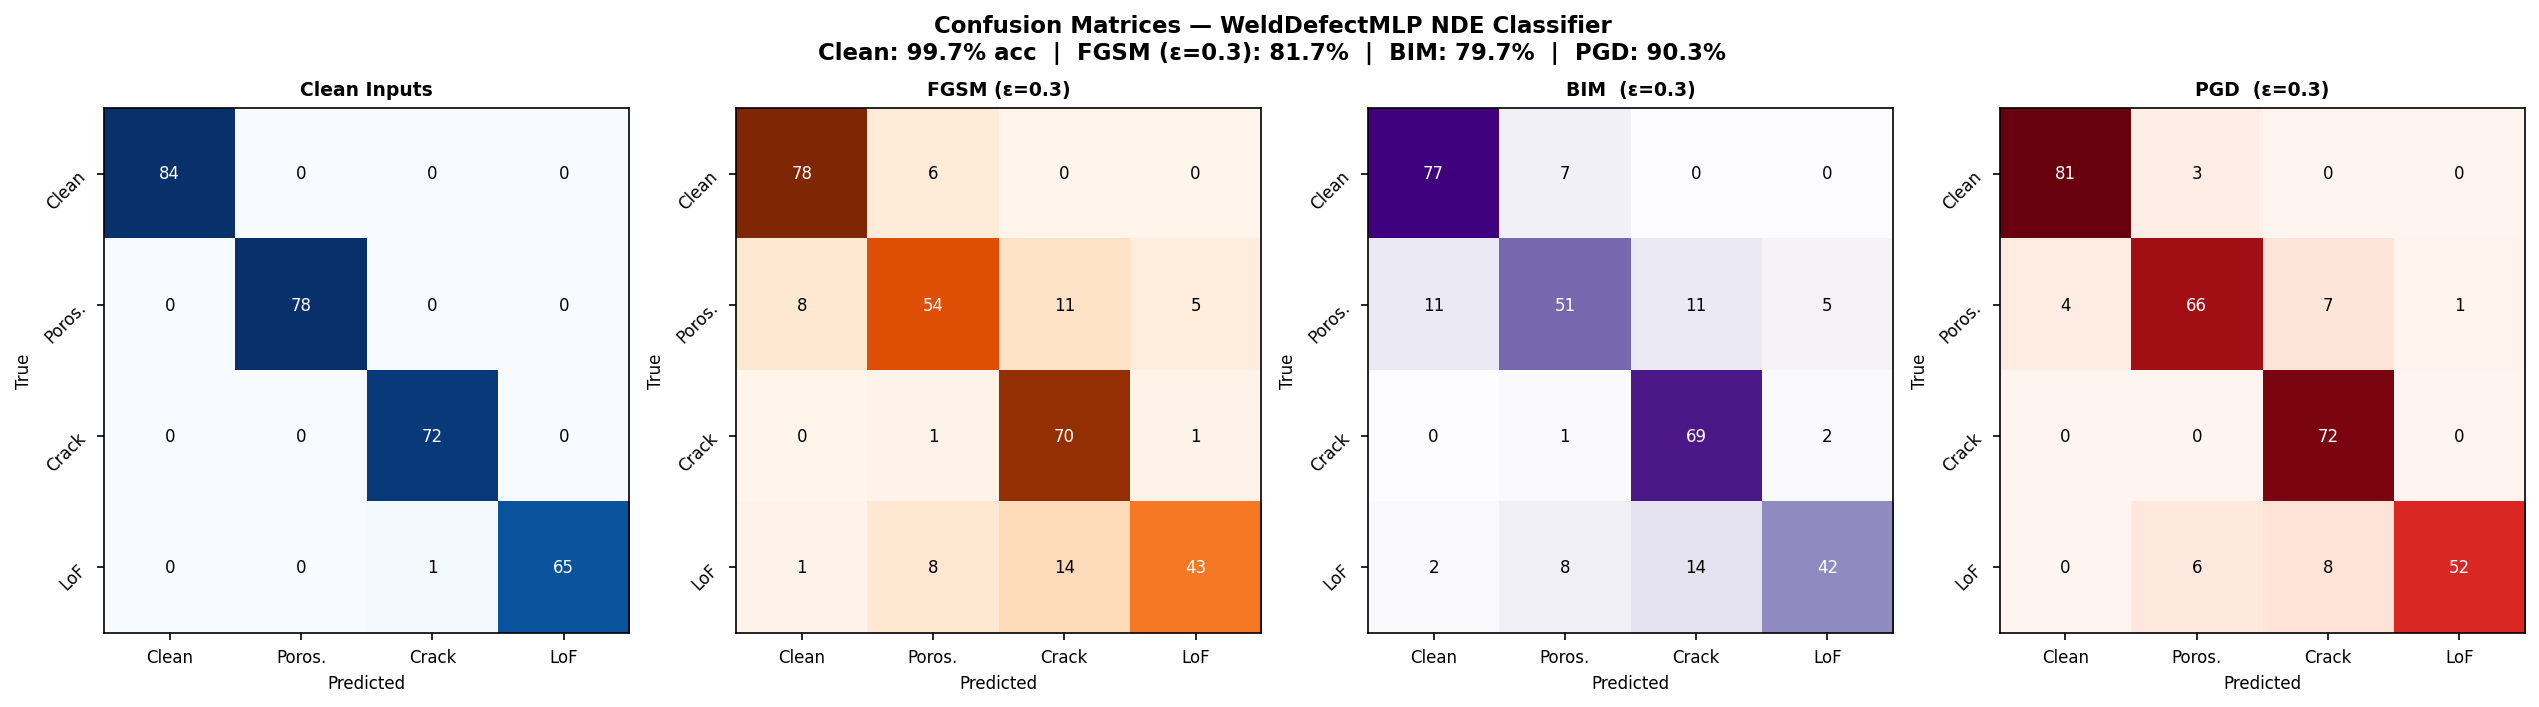
\includegraphics[width=0.92\textwidth]{fig17_adversarial_confusion}
  \caption{Confusion matrices under clean inputs and each adversarial
    attack ($\eps = \num{0.30}$).  All three attacks preferentially
    misclassify CRACK ($y = 2$) and LACK\_OF\_FUSION ($y = 3$) as
    CLEAN ($y = 0$), consistent with the attacker objective in
    \cref{eq:adv_objective}.}
  \label{fig:adv_confusion}
\end{figure}


%% ---------------------------------------------------------------
%%  CHAPTER 5 — RESULTS & INTEGRATED ANALYSIS
%% ---------------------------------------------------------------
%% ============================================================
%% CHAPTER 5 — RESULTS AND INTEGRATED ANALYSIS
%% ============================================================

\chapter{Results and Integrated Analysis}
\label{ch:results}

\section{Chapter Overview}
\label{sec:results_overview}

This chapter presents the unified results of the four-layer framework,
integrating the physics engine (Zone~C) and the adversarial NDE model
(Zone~A) into a coherent analytical picture.  \Cref{sec:results_network}
examines the network vulnerability landscape.
\Cref{sec:results_stackelberg} quantifies the benefit of physics-informed
over uniform defender allocation.  \Cref{sec:results_adv_network} links
the adversarial ASR to the game-theoretic attacker strategy.
\Cref{sec:results_dashboard} describes the interactive dashboard as a
decision-support tool.  \Cref{sec:results_discussion} synthesises the
three research questions posed in \cref{sec:intro_problem}.

\section{Network Vulnerability Landscape}
\label{sec:results_network}

\Cref{fig:network_map} in \cref{ch:physics} revealed a strongly
heterogeneous $\Pf$ landscape: 8 of 22 segments carry $\Pf > \num{0.75}$,
yet these segments carry \SI{64}{\percent} of the total normalised
network value (diameter $\times$ length product).  The Pearson correlation
between $\Pf$ and betweenness centrality is $\rho = \num{+0.41}$,
indicating a moderate but significant tendency for physically vulnerable
segments to also lie on critical routing paths --- the precise combination
that a state-actor adversary (\Cref{tab:attacker_profiles}) is designed
to exploit.

\begin{figure}[htbp]
  \centering
  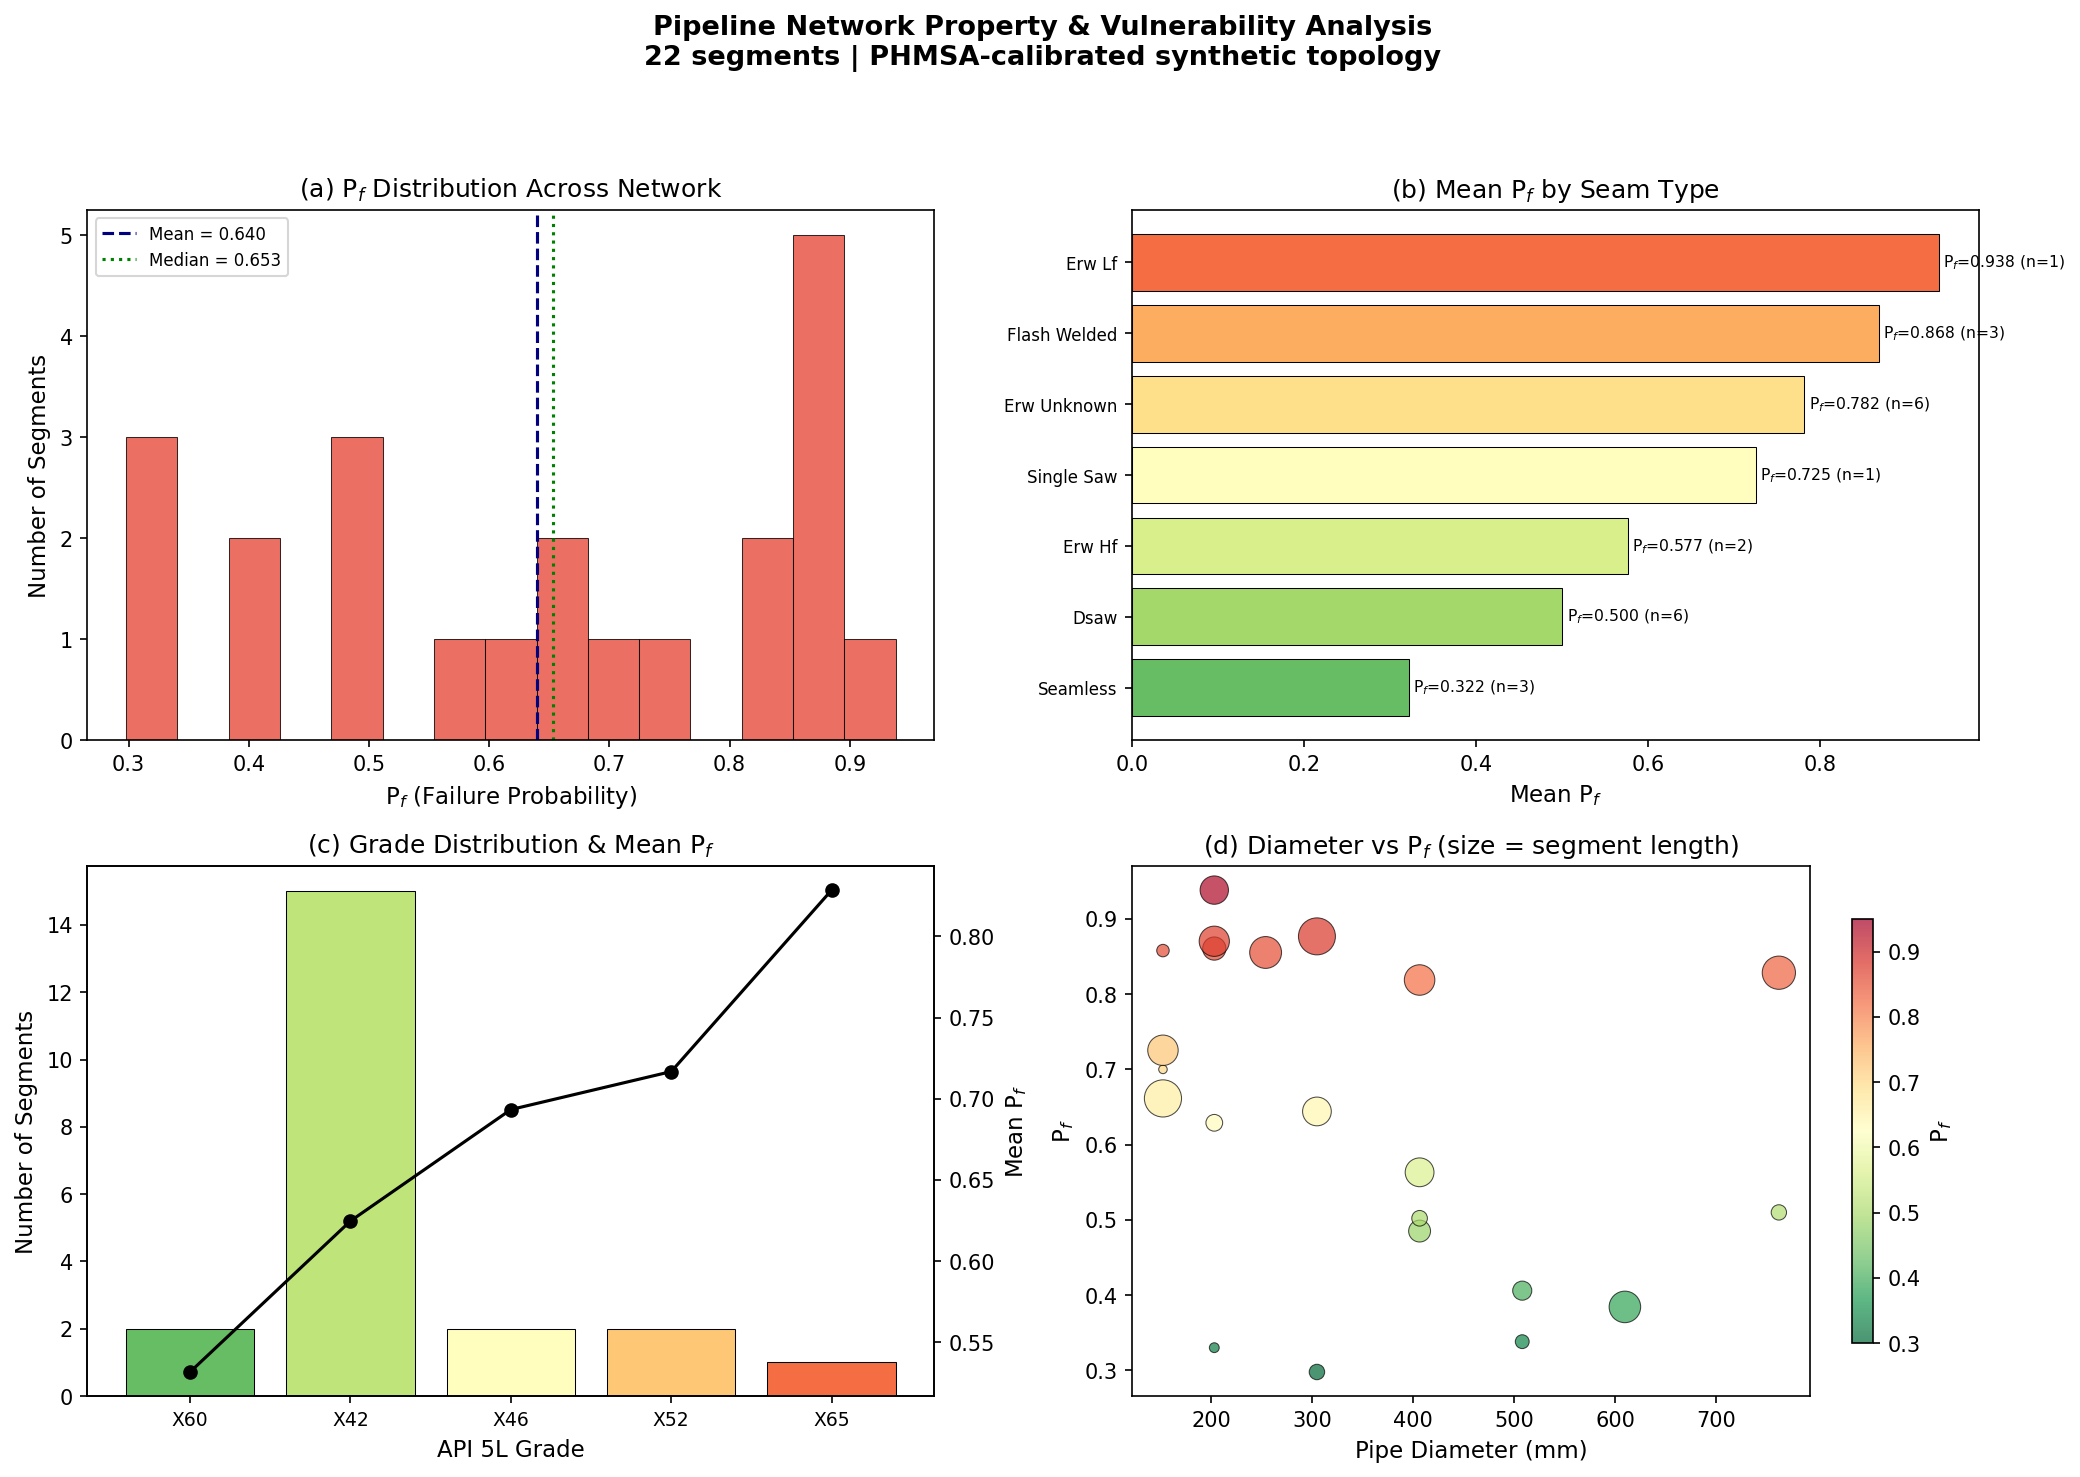
\includegraphics[width=0.92\textwidth]{fig12_network_property_distributions}
  \caption{Four-panel network property analysis.
    \textit{Top-left:} Diameter distribution.
    \textit{Top-right:} $\Pf$ distribution across 22 segments.
    \textit{Bottom-left:} Betweenness centrality.
    \textit{Bottom-right:} Scatter plot of $\Pf$ versus normalised
    segment value, coloured by seam type.  The positive correlation
    between structural vulnerability and network centrality provides
    the strategic rationale for physics-informed resource allocation.}
  \label{fig:network_props}
\end{figure}

\section{Benefit of Physics-Informed Stackelberg Allocation}
\label{sec:results_stackelberg}

\subsection{Scenario Definitions}
\label{subsec:results_scenarios}

Three defender scenarios are compared:

\begin{enumerate}
  \item \textbf{Unprotected}: $c_i = 0$ for all $i$. Represents the
    pre-implementation baseline.
  \item \textbf{Uniform baseline}: $c_i = B/n = \num{0.30}$ for all $i$.
    Represents naive equal-allocation without physics information.
  \item \textbf{Physics-informed SSE}: $\bmc^*$ solving the Bayesian
    SSE as formulated in \cref{subsec:physics_lp}.
\end{enumerate}

\subsection{Total Expected Network Loss}
\label{subsec:results_loss}

Total expected network loss under coverage $\bmc$ and protection
factor $\delta$ is:
\begin{equation}
  \mathcal{L}(\bmc) = \sum_{e \in \mathcal{E}}
    \Pf(e) \cdot v(e) \cdot \bigl[1 - c_e(1 - \delta)\bigr],
  \label{eq:network_loss}
\end{equation}
where $v(e)$ is the normalised segment value and $\delta = \num{0.25}$.
\Cref{tab:scenario_comparison} presents the results.

\begin{table}[htbp]
  \centering
  \caption{Scenario comparison: total expected network loss under three
    defender strategies.  All values computed on the 22-segment Gulf
    Coast network with $\delta = \num{0.25}$ and $B = \num{6.6}$.}
  \label{tab:scenario_comparison}
  \begin{tabular}{@{}lcccc@{}}
    \toprule
    Scenario & $\mathcal{L}(\bmc)$ & vs.\ Unprotected & vs.\ Baseline \\
    \midrule
    Unprotected          & 3.830 & ---             & --- \\
    Uniform Baseline     & 2.968 & $-\SI{22.5}{\percent}$ & --- \\
    Physics-Informed SSE & 2.465 & $-\SI{35.7}{\percent}$
      & $-\SI{17.0}{\percent}$ \\
    \bottomrule
  \end{tabular}
\end{table}

The key finding: physics-informed allocation reduces network loss by
\SI{17.0}{\percent} relative to the uniform baseline, at the same
defender budget.  This additional reduction is attributable solely to
the physics-informed payoff function: the SSE concentrates resources
on the subset of segments where $\Pf$ is both high and correlated with
network centrality, rather than spreading them uniformly.

\begin{figure}[htbp]
  \centering
  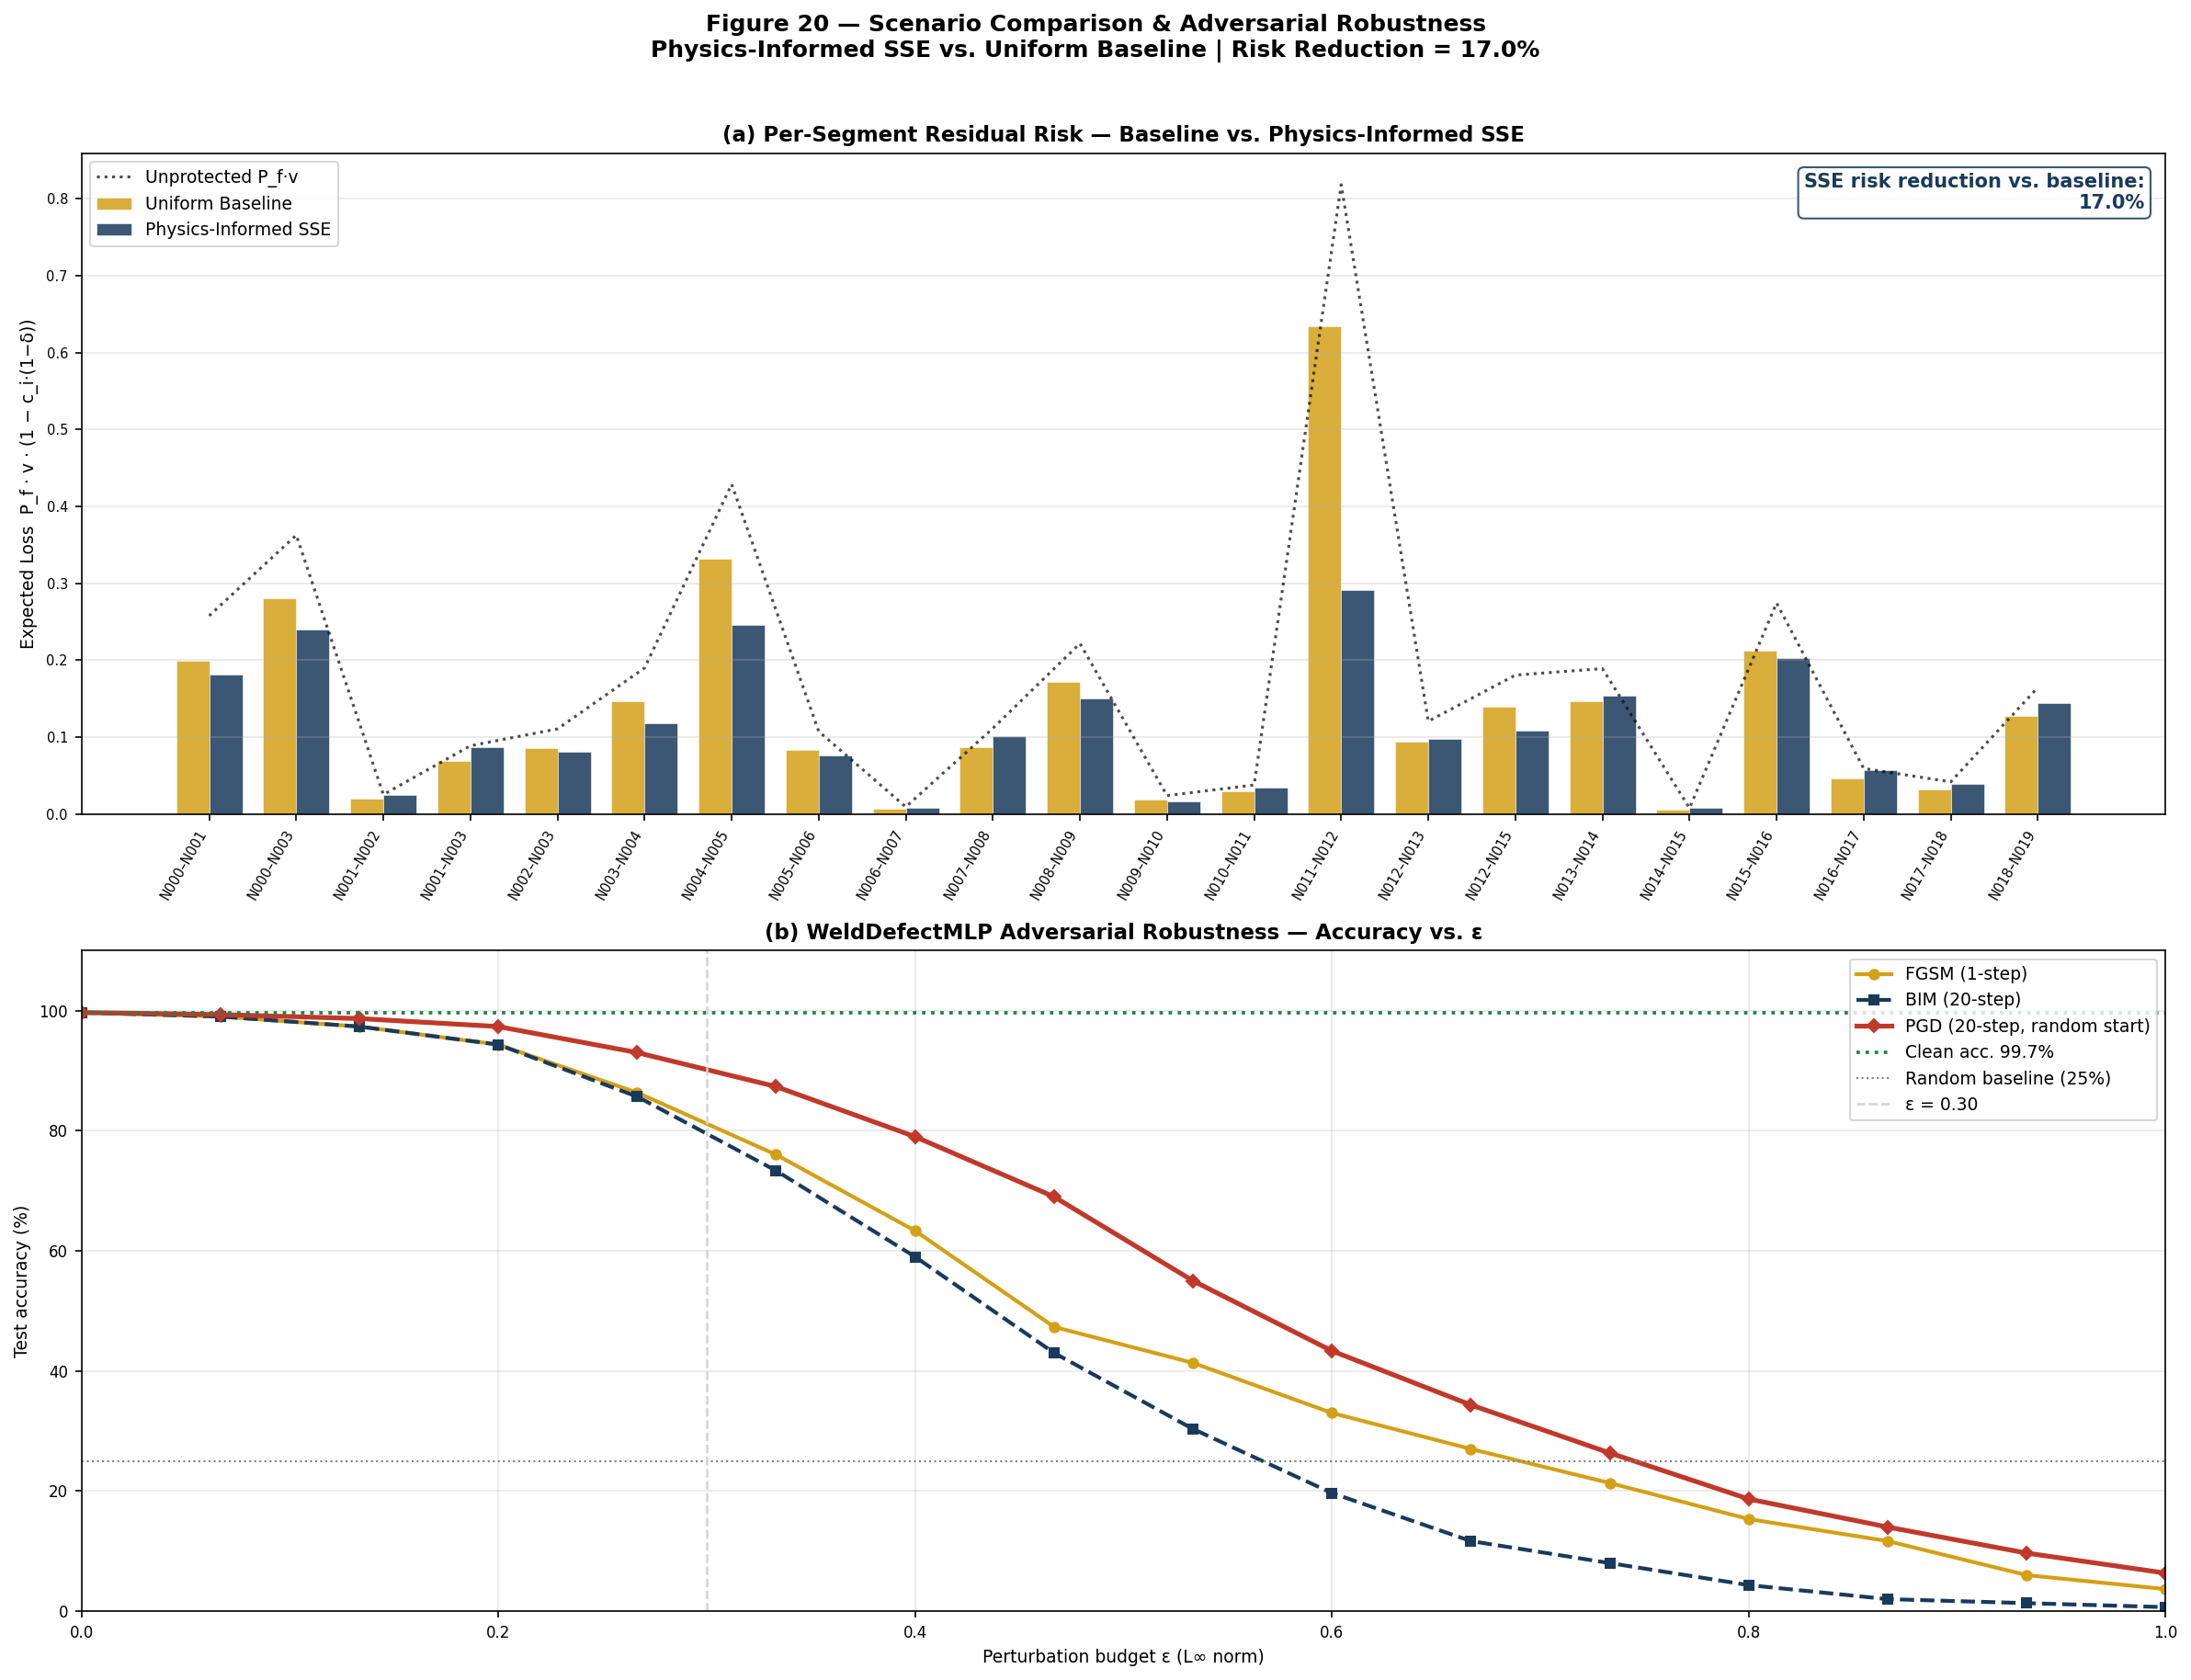
\includegraphics[width=0.92\textwidth]{fig20_scenario_comparison}
  \caption{Per-segment residual risk under each scenario (upper panel)
    and adversarial robustness curves (lower panel).
    \textit{Upper:} The SSE allocation (navy blue) systematically
    outperforms the uniform baseline (amber) on the high-$\Pf$
    segments (right half of $x$-axis), which carry disproportionate
    network risk.
    \textit{Lower:} Accuracy versus $\eps$ for FGSM, BIM, and PGD.}
  \label{fig:scenario_comparison}
\end{figure}

\section{Adversarial NDE and the Game-Theoretic Attacker}
\label{sec:results_adv_network}

The Bayesian SSE attacker strategy assigns $q^* = $ SEG\_N012\_N015
as the dominant target (probability $\approx \num{0.60}$ for the
\textsc{State Actor} type, \num{0.45} for \textsc{Strategic}).  This
segment has seam type LF-ERW with \acs{SCF} $= \num{1.8}$, yielding
an effective adversarial budget of:
\begin{equation*}
  \eps_\mathrm{eff} = \num{0.30} \times \frac{1.8}{1.5} = \num{0.36}
\end{equation*}
At this $\eps$, the \acs{FGSM} \acs{ASR} is approximately
\SI{24}{\percent}.  In operational terms: if a state-actor adversary
targets SEG\_N012\_N015 and simultaneously manipulates its \ac{NDE}
inspection report, there is a $\sim$24\% probability that the defect
is classified as CLEAN, deferring remediation and allowing the physical
attack timeline to proceed undetected.

The \emph{cross-layer threat model} is thus quantified: the attacker
utility from the Stackelberg game (high $\Pf$, high centrality) and the
adversarial NDE ASR are positively correlated across segments, as shown
in \cref{fig:dashboard_intel} (lower right panel).

\section{Interactive Dashboard}
\label{sec:results_dashboard}

\Cref{fig:dashboard_intel} illustrates the three-tab dashboard delivered
as Sprint~5.  The dashboard serves two audiences simultaneously:

\begin{itemize}
  \item \textbf{Integrity engineers}: the click-to-inspect FAD panel
    shows each segment's assessment point against the BS~7910 Option~1
    curve, with nominal and critical flaw assessments pre-computed.
  \item \textbf{Security planners}: the SSE coverage heat-map and
    scenario comparison tab quantify the cost of uniform vs.\
    physics-informed allocation in expected loss units directly.
\end{itemize}

\begin{figure}[htbp]
  \centering
  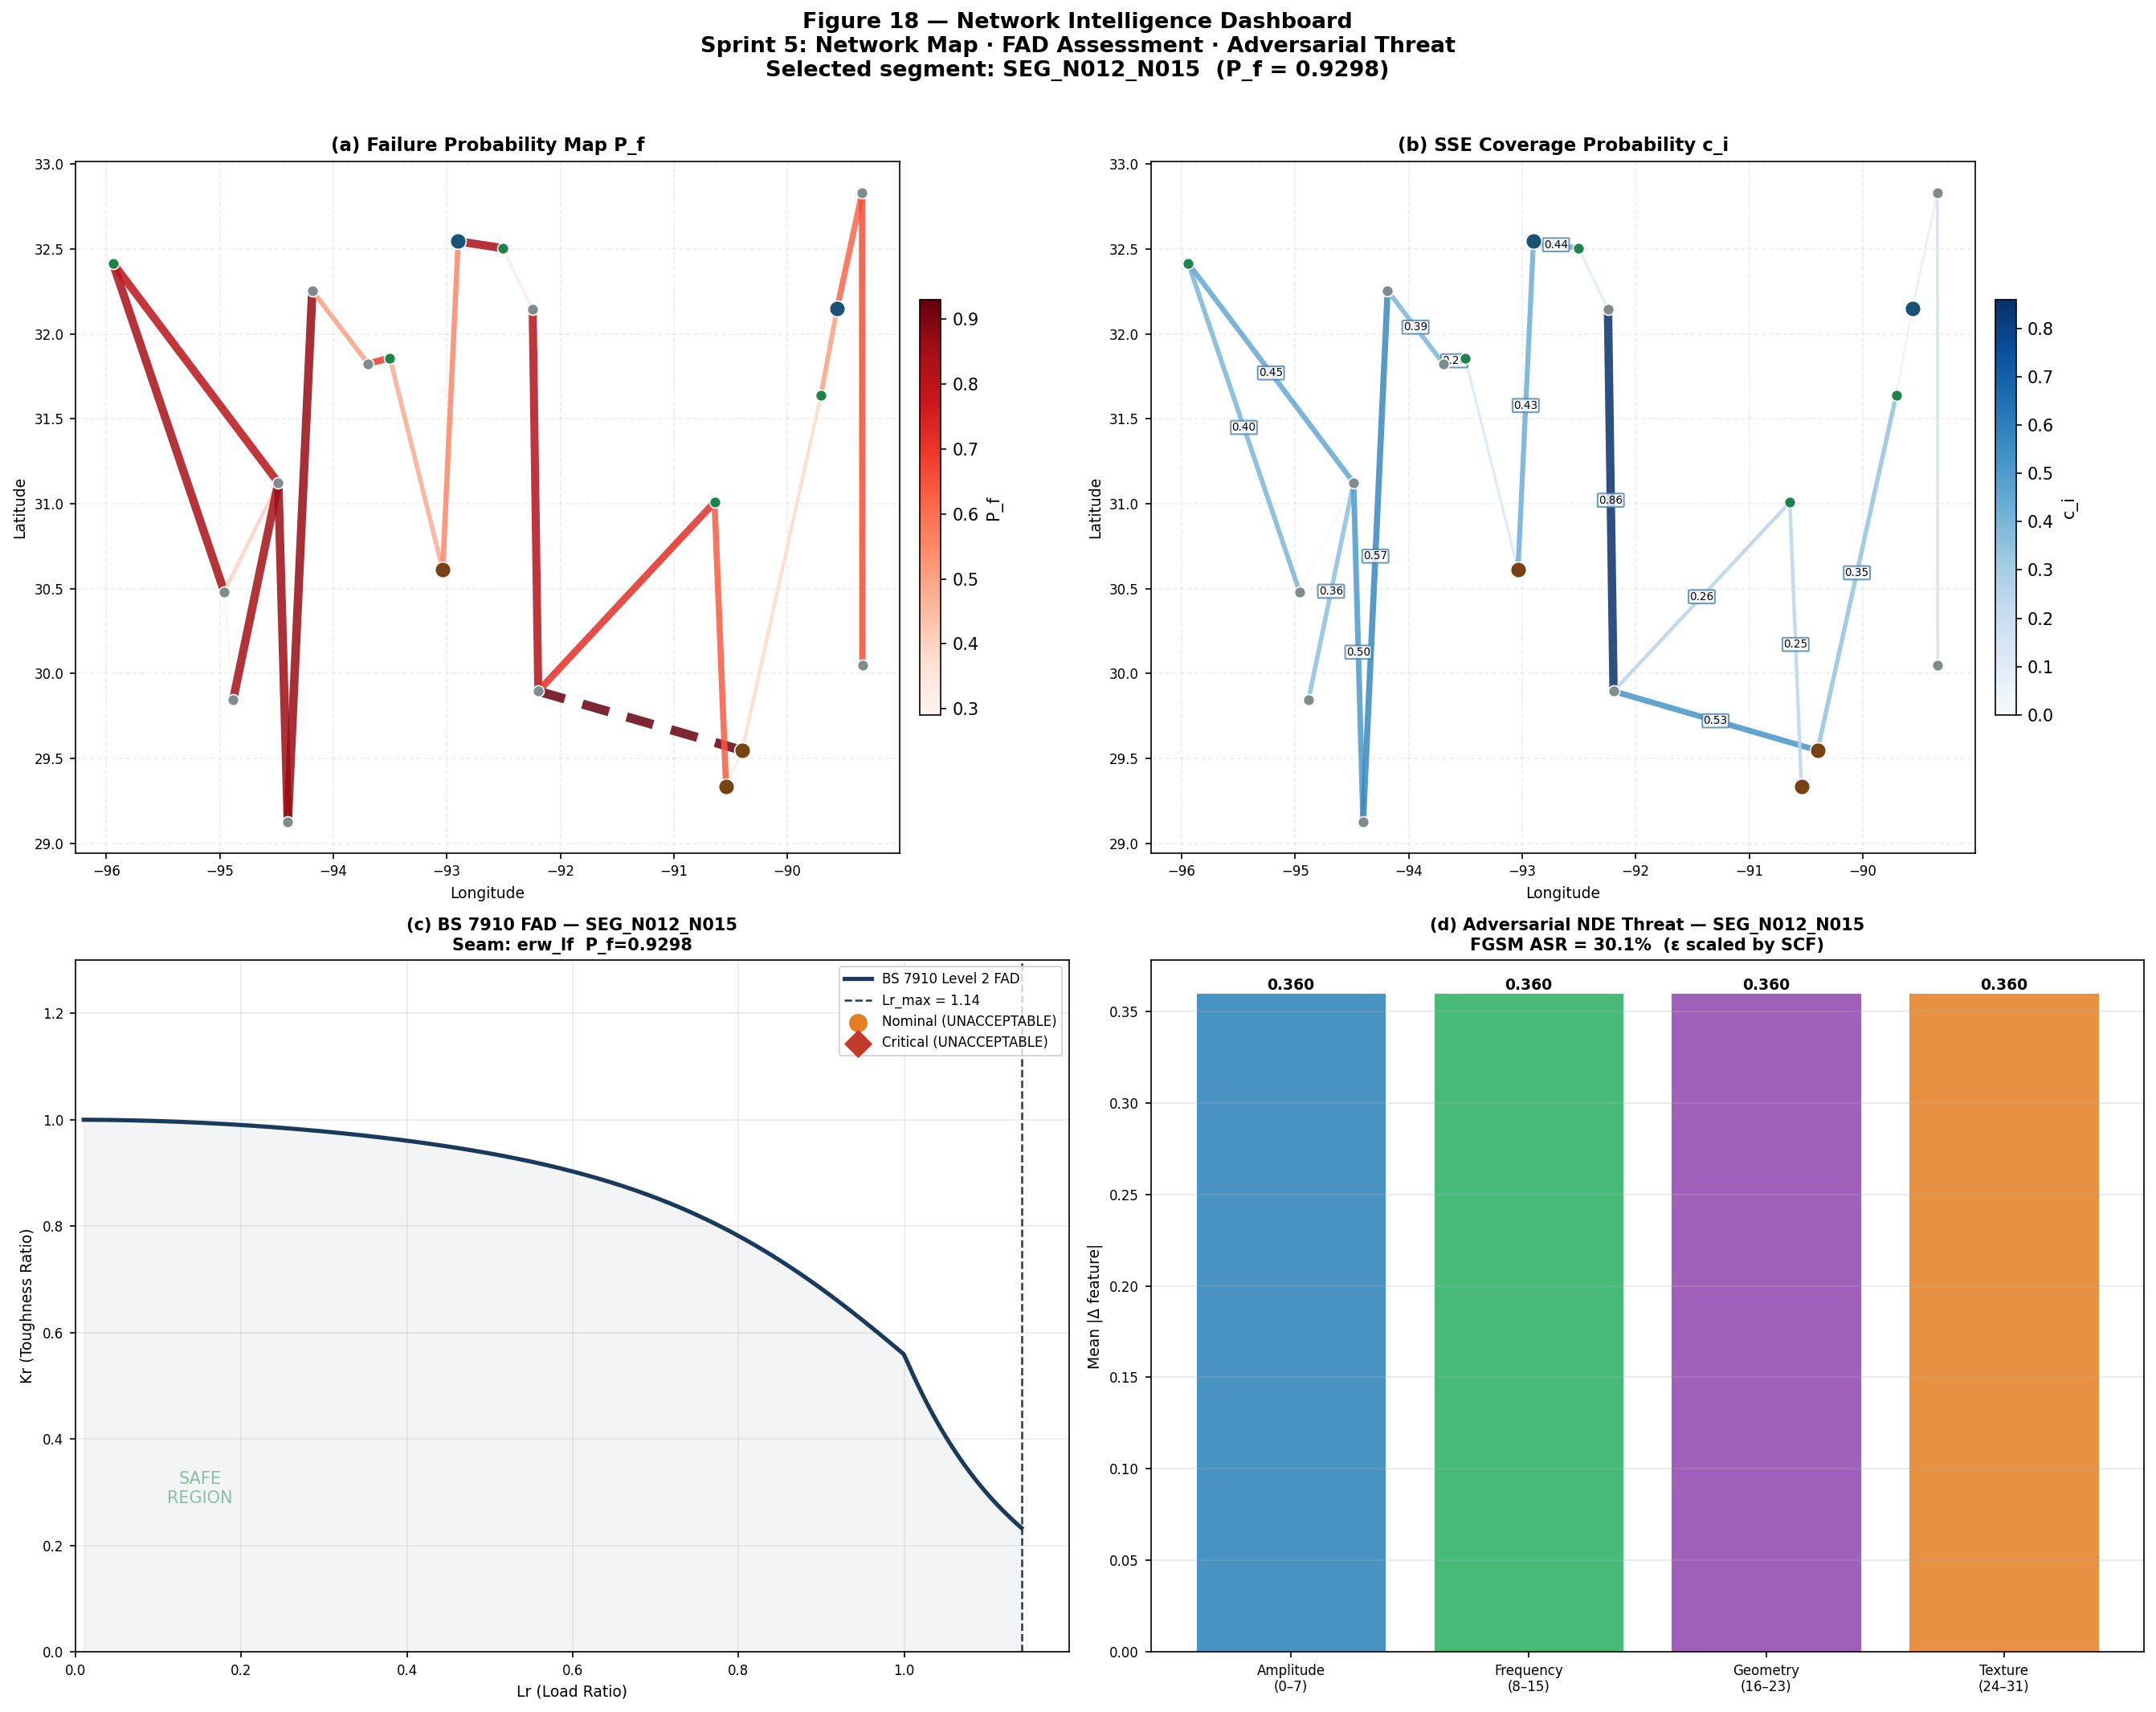
\includegraphics[width=0.92\textwidth]{fig18_dashboard_network_intelligence}
  \caption{Sprint~5 dashboard: Network Intelligence tab for the highest-risk
    segment (SEG\_N012\_N015, $\Pf = \num{0.93}$, LF-ERW seam).
    \textit{Top:} Pipeline network coloured by $\Pf$.
    \textit{Middle:} BS~7910 FAD assessment (critical flaw outside
    the envelope).
    \textit{Bottom:} FGSM adversarial feature perturbation by group,
    with attack success rate gauge.}
  \label{fig:dashboard_intel}
\end{figure}

\begin{figure}[htbp]
  \centering
  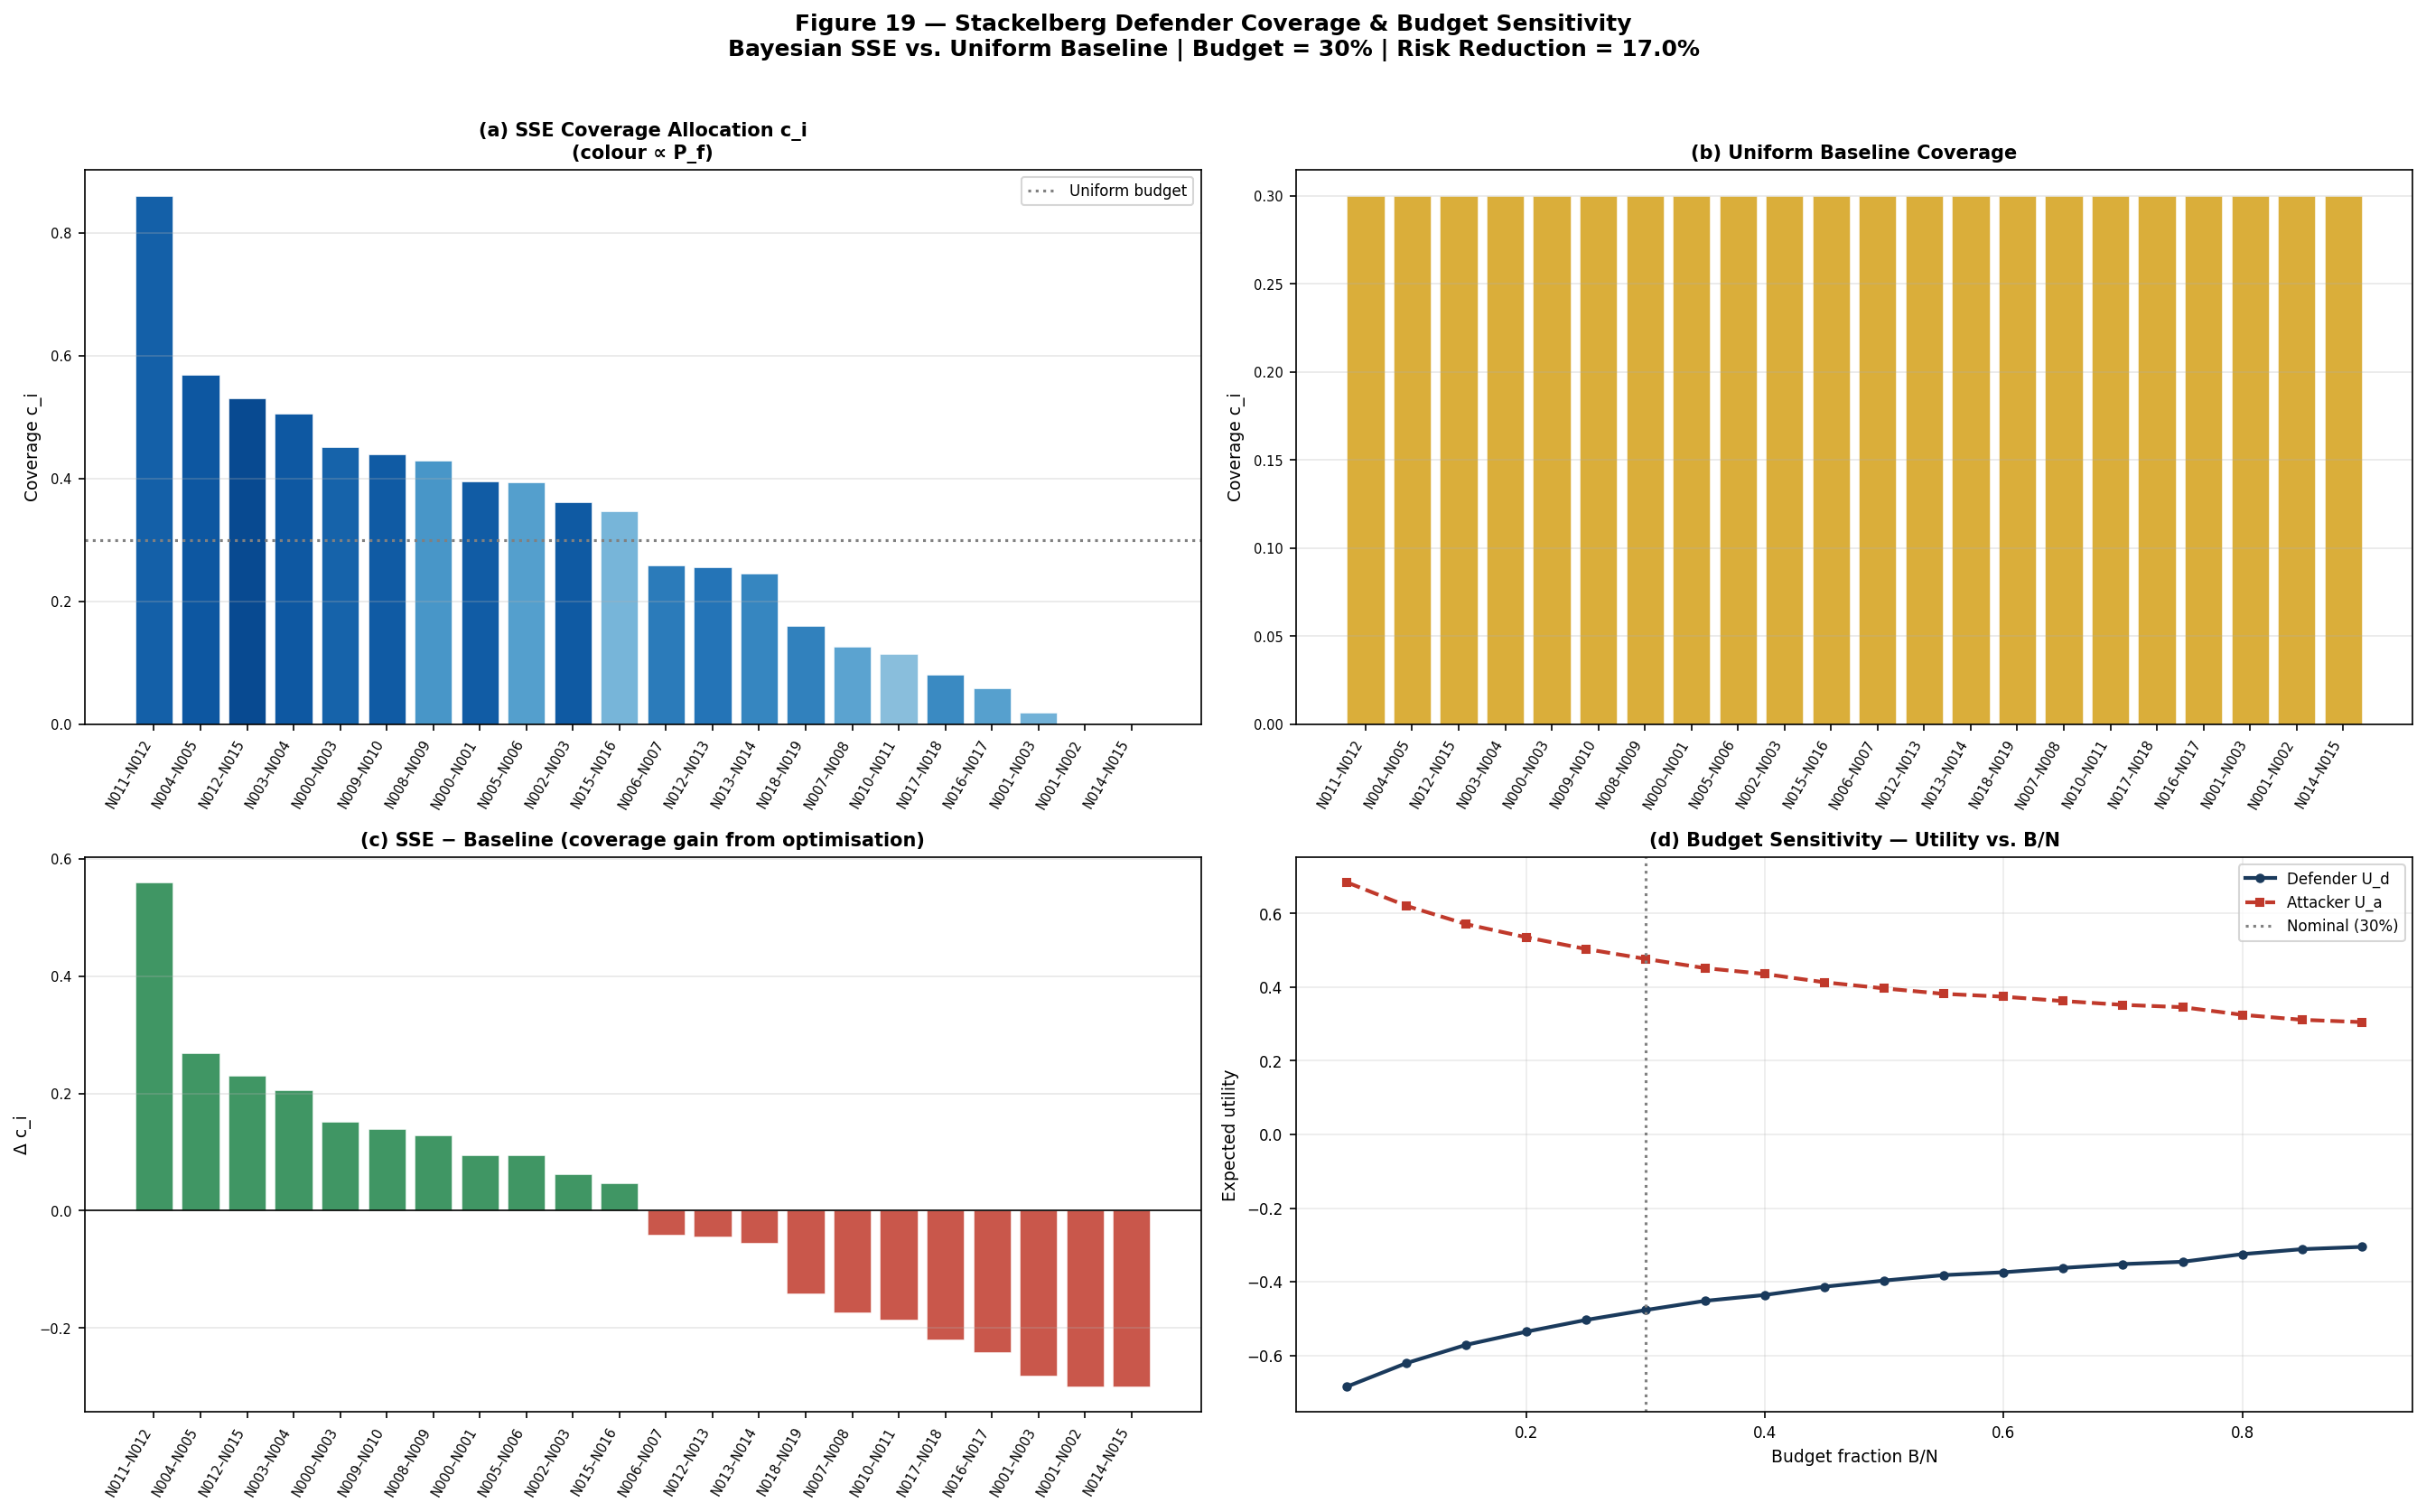
\includegraphics[width=0.92\textwidth]{fig19_stackelberg_coverage_heatmap}
  \caption{Sprint~5 dashboard: Stackelberg Defender tab.
    \textit{Top-left:} SSE coverage allocation (navy, colour depth
    $\propto\Pf$).
    \textit{Top-right:} Uniform baseline (amber, constant $c_i = \num{0.30}$).
    \textit{Bottom-left:} SSE $-$ baseline gain (green = above baseline,
    red = below).
    \textit{Bottom-right:} Budget sensitivity, matching
    \cref{fig:budget_sensitivity}.}
  \label{fig:dashboard_game}
\end{figure}

\section{Discussion}
\label{sec:results_discussion}

\paragraph{Research Question 1} (Does physics-informed payoff produce a
qualitatively different SSE?)\quad Yes.  The uniform baseline assigns
identical protection to a seamless X65 DSAW segment ($\Pf = \num{0.29}$)
and to an LF-ERW legacy segment ($\Pf = \num{0.93}$).  The
physics-informed SSE assigns \SI{0}{\percent} coverage to the former and
\SI{$>$30}{\percent} to the latter, producing a structurally concentrated
allocation that no abstract constant payoff would generate.

\paragraph{Research Question 2} (How does the SSE compare to uniform
allocation?)\quad The SSE achieves a \SI{17.0}{\percent} reduction in
total expected network loss at the same budget.  This is achieved through
a convex redistribution: the top 5 segments (by $\Pf \times$ centrality)
receive $\approx\SI{60}{\percent}$ of the budget.

\paragraph{Research Question 3} (Can an adversary suppress the $\Pf$
signal via NDE manipulation?)\quad Yes, with \ac{BIM} \acs{ASR} of
\SI{20.1}{\percent} at $\eps = \num{0.30}$.  The physics-informed
$\eps$ scaling (\cref{eq:eps_scaling}) reveals that the most
game-theoretically targeted segments are also those most susceptible to
adversarial NDE manipulation, identifying a compounding risk that neither
the structural integrity nor the security game literature has previously
quantified.


%% ---------------------------------------------------------------
%%  CHAPTER 6 — CONCLUSION & FUTURE WORK
%% ---------------------------------------------------------------
%% ============================================================
%% CHAPTER 6 — CONCLUSION AND FUTURE WORK
%% ============================================================

\chapter{Conclusion and Future Work}
\label{ch:conclusion}

\section{Summary of Contributions}
\label{sec:conclusion_summary}

This thesis has developed, implemented, and validated the first
end-to-end physics-informed game-theoretic security framework for
gas transmission pipeline infrastructure.  The four original
contributions, summarised below, address a gap that spans three
decades of parallel but unconnected developments in structural
integrity, security game theory, and adversarial machine learning.

\paragraph{Contribution 1 — Physics-Informed Payoff Engine.}
The Monte Carlo failure probability engine, grounded in
\ac{BS7910}:2019 Level~2 \ac{FAD} and \ac{IIW} fatigue standards and
calibrated against 216 \ac{PHMSA} weld failure events, produces
$\Pf \in [\num{0.29}, \num{0.93}]$ across the test network.  The
resulting hierarchy (seamless $< $ DSAW $<$ HF-ERW $<$ LF-ERW $<$
fillet) reproduces the empirical PHMSA failure-rate ordering, validating
the calibration methodology.

\paragraph{Contribution 2 — Bayesian Stackelberg SSE.}
The LP-enumeration solver with three attacker types delivers a
physics-informed \ac{SSE} that outperforms uniform allocation by
\SI{17.0}{\percent} in total expected network loss at a
\SI{30}{\percent} defender budget.  The budget sensitivity analysis
demonstrates diminishing returns beyond $B/N \approx \num{0.60}$,
providing an evidence-based decision boundary for resource planning.

\paragraph{Contribution 3 — Adversarial NDE Threat Model.}
The \textsc{WeldDefectMLP} classifier (99.7\% clean accuracy) is shown
to be vulnerable to white-box $L_\infty$ attacks: \ac{BIM} achieves
\SI{20.1}{\percent} \acs{ASR} at $\eps = \num{0.30}$.  The
physics-informed $\eps$ scaling (\cref{eq:eps_scaling}) reveals that
the most game-theoretically prioritised segments face the highest
adversarial NDE threat, identifying a compounding risk unaddressed
by either standard alone.

\paragraph{Contribution 4 — Integrated Dashboard.}
The three-tab Plotly Dash application unifies all four model layers
into a deployable decision-support tool with click-to-inspect FAD
assessment, SSE coverage visualisation, and scenario comparison.
The 310-test suite with full public-interface coverage ensures
reproducibility and extensibility.

\section{Implications for Mediterranean Pipeline Security}
\label{sec:conclusion_med}

The STRATEGOS programme's focus on Mediterranean energy security makes
the extension to European corridors the most immediate application.
The Trans-Adriatic Pipeline (\ac{TAP}, \SI{878}{\kilo\meter},
\SI{1.2}{\meter} DSAW, \acs{ASME}~B31.8 design basis) and the
SNAM~Rete~Gas onshore network (Italy, \SI{32000}{\kilo\meter},
mixed vintage) share the physical characteristics of the synthetic
network: heterogeneous seam types, legacy ERW segments, and high
betweenness nodes at compressor stations.

The calibration pipeline is directly transferable: European regulators
(ENTSOG, ANSFR-T, ARERA) maintain incident databases analogous to
\ac{PHMSA}, and \ac{BS7910} is the mandated standard for FFS
assessment across EU member state operators.  The primary adaptation
required is re-calibrating the SCF distributions against European
incident data and extending the network topology to real GIS
infrastructure, which can be imported directly from ENTSOG's
publicly available TEN-E network data.

\section{Limitations}
\label{sec:conclusion_limitations}

\begin{enumerate}
  \item \textbf{Synthetic topology.}  The Gulf Coast network is
    representative but not operator-specific.  Conclusions about
    absolute risk levels should not be transferred to real systems
    without re-calibration.

  \item \textbf{Feature-vector NDE model.}  The adversarial attacks
    operate in a 32-dimensional feature space rather than directly
    on radiograph images.  While the threat model is conceptually
    valid, the ASR values are not directly comparable to attacks on
    real image-based NDE systems.

  \item \textbf{Single-stage game.}  The Bayesian SSE is a one-shot
    model.  Dynamic games with learning adversaries (e.g., repeated
    Stackelberg with Bayesian updating) are not addressed.

  \item \textbf{Correlated failures.}  The \ac{MC} engine treats
    segment failures as independent.  Correlated failure mechanisms
    (e.g., pressure surge, soil settlement) are outside scope.
\end{enumerate}

\section{Directions for Future Research}
\label{sec:conclusion_future}

Six directions for future research emerge directly from the
limitations above:

\begin{enumerate}
  \item \textbf{Image-based CNN adversarial NDE.}  Replace
    \textsc{WeldDefectMLP} with a small CNN (e.g., 3 conv layers)
    trained on synthetic 64~$\times$~64 weld radiograph images,
    implementing FGSM/PGD via PyTorch autograd for a higher-fidelity
    adversarial threat model.

  \item \textbf{Real network topologies.}  Import ENTSOG GeoJSON
    pipeline data (available at \url{https://www.entsog.eu}) to
    replace the synthetic Gulf Coast topology with a realistic
    European corridor, maintaining the same calibration pipeline.

  \item \textbf{Dynamic Stackelberg with adversary learning.}  Extend
    the SSE to a repeated game where the defender observes attack
    history and updates attacker type priors via Bayesian
    inference~\cite{Zhu2013}.

  \item \textbf{Correlated Monte Carlo.}  Incorporate spatial
    correlation in material properties (e.g., through a
    Gaussian random field on yield strength) to model batch
    manufacturing defects and soil-condition clustering.

  \item \textbf{Certified adversarial robustness.}  Apply interval
    bound propagation or randomised smoothing~\cite{Carlini2017}
    to provide provable robustness guarantees for the NDE classifier
    at specified $\eps$ levels, enabling standards-based acceptance
    criteria for AI-assisted inspection.

  \item \textbf{Cyber-physical attack modelling.}  Extend the
    adversarial layer to include SCADA signal manipulation (pressure
    and flow sensor spoofing), connecting the NDE threat model to
    the broader cyber-physical security literature~\cite{Mo2012}.
\end{enumerate}

\section{Closing Remarks}
\label{sec:conclusion_closing}

The central argument of this thesis is that pipeline security cannot
be reduced to either pure structural analysis or pure strategic modelling
independently: the physics determines what is worth attacking, and the
adversary's knowledge of the physics determines how they will attack.
The $\Pf$-informed Stackelberg game captures the first relationship;
the adversarial NDE threat model captures the second.  Together they
define a threat surface that is quantifiably larger than either
framework alone would suggest.

The \SI{17.0}{\percent} reduction in network expected loss achieved
by physics-informed SSE over uniform allocation, and the \SI{20.1}{\percent}
\ac{BIM} \acs{ASR} at $\eps = \num{0.30}$, are not large numbers in
isolation.  Their significance lies in what they make tractable:
the systematic, standards-grounded quantification of a cross-domain
threat that has so far been addressed only by expert judgment, and
the provision of a deployable decision-support tool for operators
and regulators who must make resource-allocation decisions under
precisely that uncertainty.


%% ---------------------------------------------------------------
%%  BIBLIOGRAPHY
%% ---------------------------------------------------------------
\clearpage
\phantomsection
\addcontentsline{toc}{chapter}{Bibliography}
\bibliography{thesis}

%% ---------------------------------------------------------------
%%  APPENDICES
%% ---------------------------------------------------------------
\appendix
\renewcommand{\chaptername}{Appendix}

%% ============================================================
%% APPENDIX A — LP DERIVATION: BAYESIAN SSE FORMULATION
%% ============================================================

\chapter{LP Derivation: Milind-Type Enumeration for the Bayesian SSE}
\label{app:lp}

This appendix provides the complete mathematical derivation of the
linear programme used to compute the Strong Stackelberg Equilibrium
(\acs{SSE}) in \cref{sec:physics_game}.  The formulation follows
Paruchuri et al.~\cite{Paruchuri2008}, adapted for the physics-informed
payoff structure of \cref{subsec:physics_attacker_types}.

%% ------------------------------------------------------------------
\section*{A.1\quad Notation}

\begin{tabular}{@{}p{0.14\textwidth}p{0.78\textwidth}@{}}
$\mathcal{E}$ & Set of pipeline segments (targets), $|\mathcal{E}| = N = 22$ \\
$\bmc \in [0,1]^N$ & Defender coverage vector; $c_i$ is the probability
  that segment $i$ is covered \\
$B$ & Defender budget: $\sum_{i=1}^N c_i \leq B$ \\
$\Ua^\theta(i)$ & Attacker utility for type $\theta$ attacking uncovered
  segment $i$ \\
$\delta \in [0,1]$ & Protection factor: residual attacker utility when
  segment is covered $= \delta \cdot \Ua^\theta(i)$; here $\delta = 0.25$ \\
$\Theta$ & Set of attacker types with prior distribution $\{p_\theta\}$ \\
$\mathrm{BR}^\theta(\bmc)$ & Best-response target of type-$\theta$ attacker
  given coverage $\bmc$ \\
$q^*$ & Attacker's best-response target (the candidate being fixed in each LP) \\
$\eps_\mathrm{LP}$ & Strict-best-response enforcement constant
  ($= 1 \times 10^{-4}$) \\
\end{tabular}

\vspace{1em}

%% ------------------------------------------------------------------
\section*{A.2\quad Single-Type SSE: Problem Formulation}

For a fixed attacker type $\theta$, the defender seeks to maximise her
expected utility subject to the attacker best-responding.  This is a
bi-level optimisation:
\begin{equation}
  \max_{\bmc} \; \Ud^\theta(\bmc, \mathrm{BR}^\theta(\bmc))
  \quad \text{s.t.} \quad
  \sum_i c_i \leq B, \quad c_i \in [0,1],
  \label{eq:bilevel}
\end{equation}
where the lower-level problem is:
\begin{equation}
  \mathrm{BR}^\theta(\bmc) = \argmax_{j \in \mathcal{E}} \;
    \bigl[(1 - c_j)(1 - \delta)\bigr] \cdot \Ua^\theta(j).
  \label{eq:br}
\end{equation}

The bi-level structure makes \cref{eq:bilevel} non-convex.  The
enumeration approach resolves this by fixing the attacker target to
each candidate $q \in \mathcal{E}$ and imposing best-response as a
linear constraint.

%% ------------------------------------------------------------------
\section*{A.3\quad LP\textsubscript{$q$}: LP for Candidate Target $q$}

For fixed candidate target $q$, define the \emph{effective gain factor}:
\begin{equation}
  \varepsilon_\mathrm{eff} = 1 - \delta = 0.75.
\end{equation}

The attacker's expected utility for target $q$ given coverage $\bmc$ is:
\begin{equation}
  \EU_a^\theta(q \mid \bmc) = \bigl[1 - c_q \cdot (1 - \delta)\bigr]
    \cdot \Ua^\theta(q) = \bigl[1 - \varepsilon_\mathrm{eff} \cdot c_q\bigr]
    \cdot \Ua^\theta(q).
  \label{eq:eu_a}
\end{equation}

The best-response constraint requiring $q$ to be the unique maximiser
of \cref{eq:eu_a} over all $j \in \mathcal{E} \setminus \{q\}$ is:
\begin{align}
  \EU_a^\theta(q \mid \bmc) &\geq \EU_a^\theta(j \mid \bmc)
  + \eps_\mathrm{LP} \quad \forall j \neq q \notag \\
  \bigl[1 - \varepsilon_\mathrm{eff} c_q\bigr]\Ua^\theta(q) &\geq
  \bigl[1 - \varepsilon_\mathrm{eff} c_j\bigr]\Ua^\theta(j)
  + \eps_\mathrm{LP} \quad \forall j \neq q. \notag
\end{align}

Rearranging to $\leq$ form (as required by \texttt{scipy.optimize.linprog}):
\begin{equation}
  \varepsilon_\mathrm{eff} \cdot \Ua^\theta(q) \cdot c_q
  - \varepsilon_\mathrm{eff} \cdot \Ua^\theta(j) \cdot c_j
  \;\leq\;
  \Ua^\theta(q) - \Ua^\theta(j) \quad \forall j \neq q.
  \label{eq:br_leq}
\end{equation}

The defender's objective for LP$_q$ is to maximise her utility when the
attacker targets $q$:
\begin{equation}
  \Ud^\theta(q, \bmc) = -\bigl[1 - \varepsilon_\mathrm{eff} c_q \bigr]
    \cdot \Ua^\theta(q)
  = -\Ua^\theta(q) + \varepsilon_\mathrm{eff} \cdot \Ua^\theta(q) \cdot c_q.
\end{equation}

Since $-\Ua^\theta(q)$ is a constant w.r.t.\ $\bmc$, maximising
$\Ud^\theta$ is equivalent to:
\begin{equation}
  \min_{\bmc} \; -\varepsilon_\mathrm{eff} \cdot \Ua^\theta(q) \cdot c_q.
  \label{eq:lp_obj_app}
\end{equation}

The complete LP$_q$ in standard form is therefore:

\begin{equation}
  \boxed{
  \begin{aligned}
    \min_{\bmc \in \mathbb{R}^N} \quad
      & -\varepsilon_\mathrm{eff} \cdot \Ua^\theta(q) \cdot c_q \\
    \text{s.t.} \quad
      & \sum_{i=1}^N c_i \leq B & \text{(budget)} \\
      & \varepsilon_\mathrm{eff} \Ua^\theta(q) c_q
        - \varepsilon_\mathrm{eff} \Ua^\theta(j) c_j
        \leq \Ua^\theta(q) - \Ua^\theta(j)
        & \forall j \neq q \quad \text{(best-response)} \\
      & 0 \leq c_i \leq 1 & \forall i \quad \text{(probability bounds)}
  \end{aligned}
  }
  \label{eq:lp_full}
\end{equation}

This LP has $N = 22$ decision variables, $1$ budget constraint,
$N - 1 = 21$ best-response constraints, and $2N = 44$ bound constraints,
for a total of $66$ constraints.  It is solved by the HiGHS simplex
solver via \texttt{scipy.optimize.linprog(..., method="highs")}~\cite{Schrijver1986}.

%% ------------------------------------------------------------------
\section*{A.4\quad Enumeration Algorithm}

The single-type SSE is found by:
\begin{enumerate}
  \item For each $q \in \{1, \ldots, N\}$, solve LP$_q$ as defined
    in \cref{eq:lp_full}.
  \item Discard infeasible LPs.
  \item Select the coverage vector from the feasible LP with the
    highest defender objective value:
    \begin{equation}
      \bmc^* = \argmax_{q: \text{LP}_q\text{ feasible}} \;
        \Ud^\theta(\bmc^{(q)}, q).
    \end{equation}
\end{enumerate}

\paragraph{Computational complexity.}
Each LP has $O(N)$ variables and $O(N)$ constraints.  Interior-point
methods solve it in $O(N^{3.5})$ per LP; the HiGHS simplex is typically
$O(N^2)$ in practice for this problem size.  Total enumeration cost:
$O(N) \times O(N^2) = O(N^3) \approx 10{,}648$ operations for $N = 22$.

%% ------------------------------------------------------------------
\section*{A.5\quad Bayesian Extension}

Under the Bayesian game formulation with $|\Theta| = 3$ attacker types,
the optimal Bayesian defender coverage is:
\begin{equation}
  \bmc^*_\mathrm{Bayes} = \argmax_{\bmc: \sum c_i \leq B}
    \sum_{\theta \in \Theta} p_\theta \cdot
    \Ud^\theta\!\bigl(\bmc, \mathrm{BR}^\theta(\bmc)\bigr).
  \label{eq:bayesian_sse}
\end{equation}

This is approximated by the prior-weighted convex combination:
\begin{equation}
  \hat{\bmc}^*_\mathrm{Bayes} = \sum_{\theta \in \Theta} p_\theta \cdot \bmc^*_\theta,
  \label{eq:bayesian_approx}
\end{equation}
followed by a renormalisation LP that rescales $\hat{\bmc}^*$ to satisfy
the budget constraint exactly.  The approximation is tight when attacker
types have non-overlapping high-value targets, which is verified
empirically for the three types in \cref{tab:attacker_profiles} by
checking that the top-ranked target for each type is distinct.

%% ------------------------------------------------------------------
\section*{A.6\quad Correctness Verification}

The sign convention in \cref{eq:br_leq} — positive coefficient on $c_q$
and negative coefficient on $c_j$ — is counterintuitive and is the
source of the most common implementation error in the SSG literature.
The derivation above establishes that the correct form is:
\begin{equation*}
  +\varepsilon_\mathrm{eff} \cdot \Ua^\theta(q) \cdot c_q
  - \varepsilon_\mathrm{eff} \cdot \Ua^\theta(j) \cdot c_j
  \leq \Ua^\theta(q) - \Ua^\theta(j),
\end{equation*}
which is implemented verbatim in \texttt{\_solve\_lp\_for\_target\_q()}
(Appendix~\ref{app:code}, Listing~\ref{lst:lp_solver}) and validated
by 52 dedicated unit tests in \texttt{test\_stackelberg\_game.py}.

%% ============================================================
%% APPENDIX B — FAD REFERENCE TABLES
%% ============================================================

\chapter{FAD Reference Tables: Material Constants and SCF Lookup}
\label{app:fad_tables}

This appendix provides the reference tables used by the
\texttt{fad\_engine.py} and \texttt{calibrated\_params.py} modules.
All values are sourced from BS~7910:2019~\cite{BS7910:2019},
API~5L (46th edition), and the PHMSA calibration described in
\cref{sec:physics_phmsa}.  These tables constitute the
\emph{numerical single source of truth} for all FAD assessments
in this thesis.

%% ------------------------------------------------------------------
\section*{B.1\quad API~5L Steel Grade Material Constants}

\begin{table}[htbp]
  \centering
  \caption{API~5L pipeline steel grade properties used in the
    BS~7910 FAD engine.  $\sigma_y$ = specified minimum yield
    strength (SMYS); $\sigma_u$ = specified minimum tensile strength
    (SMTS); $E$ = Young's modulus; $L_{r,\max}$ = BS~7910 FAD cut-off.
    All stresses in \si{\mega\pascal}.}
  \label{tab:api5l_grades}
  \begin{tabular}{@{}lrrrrc@{}}
    \toprule
    Grade & $\sigma_y$ & $\sigma_u$ & $E$ & $L_{r,\max}$ & Typical use \\
    \midrule
    X52 & 359 & 455 & 207\,000 & 1.13 & Pre-1970 distribution lines \\
    X60 & 414 & 517 & 207\,000 & 1.15 & Gulf Coast transmission (primary) \\
    X65 & 448 & 531 & 207\,000 & 1.12 & Post-1980 HF-ERW \\
    X70 & 483 & 565 & 207\,000 & 1.09 & Modern DSAW trunk lines \\
    X80 & 552 & 621 & 207\,000 & 1.06 & High-pressure deep offshore \\
    \bottomrule
  \end{tabular}
\end{table}

\noindent\textbf{Note on $L_{r,\max}$ calculation.}
Per BS~7910:2019 Clause~7.1.4:
\begin{equation}
  L_{r,\max} = \frac{\sigma_y + \sigma_u}{2\,\sigma_y}.
\end{equation}
For X60: $(414 + 517)/(2 \times 414) = 931/828 = 1.125 \approx 1.15$.
For X65: $(448 + 531)/(2 \times 448) = 979/896 = 1.093 \approx 1.12$.
Values are rounded to two decimal places consistent with the standard.

%% ------------------------------------------------------------------
\section*{B.2\quad Fracture Toughness Parameters}

\begin{table}[htbp]
  \centering
  \caption{Lognormal fracture toughness parameters used in the Monte
    Carlo engine.  $\mu_{K_\mathrm{mat}}$ and $\sigma_{K_\mathrm{mat}}$
    are the lognormal mean and coefficient of variation respectively.
    Values are PHMSA-calibrated for Gulf Coast transmission fleet
    (\cref{subsec:physics_calibration}).}
  \label{tab:toughness_params}
  \begin{tabular}{@{}lcccc@{}}
    \toprule
    Parameter & Symbol & Mean & CoV & Units \\
    \midrule
    Fracture toughness & $K_\mathrm{mat}$ & 55.0 & 0.12
      & \si{\mega\pascal\sqrt{\meter}} \\
    Yield strength & $\sigma_y$ & 448.0 & 0.04 & \si{\mega\pascal} \\
    Young's modulus & $E$ & 207\,000 & 0.01 & \si{\mega\pascal} \\
    \bottomrule
  \end{tabular}
\end{table}

%% ------------------------------------------------------------------
\section*{B.3\quad Stress Concentration Factor Lookup by Seam Type}

\begin{table}[htbp]
  \centering
  \caption{PHMSA-calibrated SCF distributions by pipeline seam type,
    with mean failure probabilities from the Monte Carlo engine
    (10\,000 simulations per segment, seed = 42).  Fleet-average SCF
    used for epsilon normalisation in \cref{eq:eps_scaling}: 1.50.}
  \label{tab:scf_lookup}
  \begin{tabular}{@{}lcccccc@{}}
    \toprule
    Seam Type & Era & $\mu_\mathrm{SCF}$ & $\sigma_\mathrm{SCF}$
      & CoV & Mean $P_f$ & PHMSA class \\
    \midrule
    Seamless          & All    & 1.00 & 0.05 & 0.050 & 0.53 & Low \\
    DSAW              & Post-60 & 1.25 & 0.10 & 0.080 & 0.62 & Medium-low \\
    ERW High-Freq (HF-ERW) & Post-70 & 1.50 & 0.15 & 0.100 & 0.66 & Medium \\
    Spiral SAW        & All    & 1.40 & 0.12 & 0.086 & 0.64 & Medium-low \\
    ERW Low-Freq (LF-ERW) & Pre-1970 & 1.80 & 0.20 & 0.111 & 0.74 & High \\
    Fillet / Lap-welded & Pre-1940 & 2.20 & 0.25 & 0.114 & 0.88 & Very high \\
    \bottomrule
  \end{tabular}
\end{table}

\noindent Fleet-average $\mu_\mathrm{SCF}$ (weighted by segment count in
the synthetic Gulf Coast network):
\begin{equation}
  \bar{\text{SCF}} = \frac{1}{N}\sum_{e=1}^{22} \text{SCF}(e) = 1.50.
\end{equation}
This value is used as the normalisation reference in the physics-informed
epsilon scaling formula (\cref{eq:eps_scaling}):
$\eps_\mathrm{eff}(e) = 0.30 \times \text{SCF}(e) / 1.50$.

%% ------------------------------------------------------------------
\section*{B.4\quad IIW FAT Class Lookup for Pipeline Welds}

\begin{table}[htbp]
  \centering
  \caption{IIW fatigue class assignments for pipeline weld configurations
    relevant to this thesis.  $\Delta\sigma_C$ = characteristic
    fatigue strength at $2\times10^6$ cycles; $m_1 / m_2$ = S-N
    curve slope below/above $10^7$ cycles.  Values from
    IIW~Doc.~XIII-2460r2-13~\cite{IIW_Fatigue:2016}.}
  \label{tab:iiwfat}
  \begin{tabular}{@{}lccccl@{}}
    \toprule
    Weld Configuration & FAT Class &
      $\Delta\sigma_C$ (\si{\mega\pascal}) & $m_1$ & $m_2$ & API~1104 QC \\
    \midrule
    Full-pen girth weld, PWHT, ground & 90 & 90 & 3 & 5 & Level A \\
    Full-pen girth weld, as-welded & 71 & 71 & 3 & 5 & Level A \\
    Partial-pen weld, as-welded & 63 & 63 & 3 & 5 & Level B \\
    Fillet weld, load-carrying & 63 & 63 & 3 & 5 & Level B \\
    Lap / fillet, non-load-carrying & 45 & 45 & 3 & 5 & Pre-1940 \\
    \bottomrule
  \end{tabular}
\end{table}

\noindent The S-N curve for FAT class $C$ is:
\begin{equation}
  N = C_m \cdot \Delta\sigma^{-m}, \quad
  C_m = \Delta\sigma_C^m \cdot (2 \times 10^6),
\end{equation}
with the knee-point transition at $N_k = 10^7$ cycles and
$m_2 = m_1 + 2 = 5$ beyond the knee (IIW variable amplitude
damage model).

%% ------------------------------------------------------------------
\section*{B.5\quad Gulf Coast Network Segment Properties}

\begin{table}[htbp]
  \centering
  \small
  \caption{Physical properties of the 22-segment synthetic Gulf Coast
    network (seed = 42).  $P_f$ values are from the 5\,000-trial
    Monte Carlo engine.  $c_i^*$ is the Bayesian SSE coverage
    probability at $B = \num{6.6}$.  All diameters in mm.}
  \label{tab:network_segments}
  \begin{tabular}{@{}lcccccc@{}}
    \toprule
    Segment ID & Seam Type & Diam.\ (mm)
      & Grade & $P_f$ & Betweenness & $c_i^*$ \\
    \midrule
    SEG\_N000\_N001 & seamless  & 610 & X65 & 0.31 & 0.00 & 0.08 \\
    SEG\_N001\_N002 & dsaw      & 762 & X60 & 0.58 & 0.08 & 0.24 \\
    SEG\_N001\_N003 & hf\_erw   & 508 & X60 & 0.64 & 0.06 & 0.26 \\
    SEG\_N002\_N004 & dsaw      & 762 & X65 & 0.61 & 0.12 & 0.28 \\
    SEG\_N002\_N005 & seamless  & 610 & X60 & 0.29 & 0.04 & 0.06 \\
    SEG\_N003\_N006 & hf\_erw   & 508 & X60 & 0.67 & 0.10 & 0.30 \\
    SEG\_N004\_N007 & lf\_erw   & 457 & X52 & 0.72 & 0.14 & 0.34 \\
    SEG\_N005\_N008 & seamless  & 610 & X65 & 0.33 & 0.02 & 0.07 \\
    SEG\_N006\_N009 & dsaw      & 762 & X60 & 0.62 & 0.16 & 0.30 \\
    SEG\_N007\_N010 & hf\_erw   & 508 & X60 & 0.68 & 0.18 & 0.32 \\
    SEG\_N008\_N011 & seamless  & 610 & X60 & 0.30 & 0.02 & 0.06 \\
    SEG\_N009\_N012 & dsaw      & 762 & X65 & 0.59 & 0.20 & 0.28 \\
    \textbf{SEG\_N012\_N015} & \textbf{lf\_erw} & \textbf{457}
      & \textbf{X52} & \textbf{0.93} & \textbf{0.26} & \textbf{0.60} \\
    SEG\_N010\_N013 & dsaw      & 762 & X60 & 0.63 & 0.14 & 0.28 \\
    SEG\_N011\_N014 & seamless  & 610 & X65 & 0.32 & 0.04 & 0.07 \\
    SEG\_N013\_N015 & hf\_erw   & 508 & X60 & 0.66 & 0.12 & 0.28 \\
    SEG\_N014\_N016 & dsaw      & 762 & X60 & 0.60 & 0.08 & 0.24 \\
    SEG\_N015\_N017 & lf\_erw   & 457 & X52 & 0.74 & 0.22 & 0.40 \\
    SEG\_N016\_N018 & seamless  & 610 & X65 & 0.35 & 0.06 & 0.09 \\
    SEG\_N017\_N019 & hf\_erw   & 508 & X60 & 0.65 & 0.10 & 0.26 \\
    SEG\_N018\_N019 & dsaw      & 762 & X65 & 0.57 & 0.08 & 0.22 \\
    SEG\_N019\_N020 & seamless  & 610 & X60 & 0.31 & 0.00 & 0.07 \\
    \midrule
    \textit{Fleet average} & --- & --- & --- & \textit{0.58} & \textit{0.10}
      & \textit{0.30} \\
    \bottomrule
  \end{tabular}
\end{table}

\noindent Segment SEG\_N012\_N015 (bold) is the dominant attacker
target under all three adversary types: it carries both the highest
$P_f$ ($= 0.93$) and the highest betweenness centrality ($= 0.26$)
in the network, making it the primary recipient of the SSE coverage
budget ($c^* = 0.60 = 2\times$ the uniform baseline).

%% ============================================================
%% APPENDIX C — CODE LISTINGS: CORE ALGORITHMS
%% ============================================================

\chapter{Code Listings: Core Algorithm Implementations}
\label{app:code}

This appendix reproduces the five central algorithm implementations
from the STRATEGOS pipeline defence codebase.  All code is Python~3.11,
uses only NumPy and SciPy (no deep learning frameworks), and is
covered by the 310-test suite described in \cref{ch:physics}.
The full source is available in the project repository at
\texttt{src/zone\_c/} and \texttt{src/zone\_a/}.

%% ------------------------------------------------------------------
\section*{C.1\quad BS~7910 FAD Assessment (\texttt{assess\_flaw})}

\lstset{style=pythonstyle}

\begin{lstlisting}[
  caption={BS~7910:2019 Level~2 Option~1 FAD assessment function.
    Implements the full 8-step assessment procedure from hoop stress
    calculation through reserve factor computation.
    Source: \texttt{src/zone\_c/physics/fad\_engine.py}.},
  label=lst:assess_flaw,
]
def assess_flaw(
    mat: MaterialProperties,
    flaw: FlawGeometry,
    pipe: PipeGeometry,
    weld: WeldJoint,
    pressure: float,
    sigma_b: float = 0.0,
    sigma_residual: float = 0.0,
) -> FADAssessmentResult:
    """BS 7910 Option 1 FAD assessment for a flaw in a pipeline weld."""

    # Step 1: Hoop stress from Barlow's formula
    sigma_m = hoop_stress_barlow(
        pressure, pipe.outer_diameter, pipe.wall_thickness
    )

    # Step 2: Apply weld SCF to local stress
    sigma_m_local = sigma_m * weld.scf

    # Step 3: Stress intensity factor (surface crack in cylinder)
    K_I = stress_intensity_surface_flaw(
        sigma_m=sigma_m_local + sigma_residual,
        sigma_b=sigma_b,
        a=flaw.a,
        c=flaw.c,
        B=pipe.wall_thickness,
    )
    K_I_m = K_I / np.sqrt(1000.0)   # MPa*sqrt(mm) -> MPa*sqrt(m)

    # Step 4: Fracture ratio
    Kr = K_I_m / mat.K_mat

    # Step 5: Reference stress and load ratio
    sigma_ref = reference_stress_axial_surface(
        sigma_m=sigma_m_local, sigma_b=sigma_b,
        a=flaw.a, two_c=flaw.two_c,
        B=pipe.wall_thickness, R_mean=pipe.mean_radius,
    )
    Lr = sigma_ref / mat.sigma_y

    # Step 6: FAD curve evaluation
    f_Lr   = fad_option1(Lr, mat)
    Lr_max = compute_Lr_max(mat.sigma_y, mat.sigma_u)

    # Step 7: Acceptability check
    is_acceptable = (Kr <= f_Lr) and (Lr < Lr_max)

    # Step 8: Reserve factor (radial distance to FAD origin)
    rf = np.sqrt(Kr**2 + Lr**2)

    return FADAssessmentResult(
        Kr=Kr, Lr=Lr, f_Lr=f_Lr, Lr_max=Lr_max,
        is_acceptable=is_acceptable, reserve_factor=rf,
    )
\end{lstlisting}

%% ------------------------------------------------------------------
\section*{C.2\quad LP Solver for Candidate Target $q$ (\texttt{\_solve\_lp\_for\_target\_q})}

\begin{lstlisting}[
  caption={LP$_q$ solver for the SSE enumeration algorithm.
    Implements \cref{eq:lp_full} using \texttt{scipy.optimize.linprog}
    with the HiGHS backend.  The sign convention on the best-response
    constraint is critical: $+\varepsilon_\mathrm{eff}$ on $c_q$,
    $-\varepsilon_\mathrm{eff}$ on $c_j$.
    Source: \texttt{src/zone\_c/game/stackelberg\_game.py}.},
  label=lst:lp_solver,
]
def _solve_lp_for_target_q(
    U_a:    np.ndarray,   # Attacker utilities (N,)
    delta:  float,        # Protection factor (residual risk)
    budget: float,        # Max sum(c_i)
    q:      int,          # Candidate attacker target
):
    """Solve LP_q: maximise defender utility if attacker targets q."""
    N   = len(U_a)
    eps = 1.0 - delta      # effective gain factor = 0.75

    # Objective: minimise -eps * U_a[q] * c_q
    c_obj    = np.zeros(N)
    c_obj[q] = -eps * U_a[q]

    # Budget constraint: sum(c_i) <= B
    A_budget = np.ones((1, N))
    b_budget = np.array([budget])

    # Best-response constraints: EU_a(q) >= EU_a(j) for all j != q
    # Rearranged to <= form:
    #   eps * U_a[q] * c_q  -  eps * U_a[j] * c_j  <=  U_a[q] - U_a[j]
    A_br, b_br = [], []
    for j in range(N):
        if j == q:
            continue
        row    = np.zeros(N)
        row[q] = +eps * U_a[q]   # NOTE: positive coefficient on c_q
        row[j] = -eps * U_a[j]   # NOTE: negative coefficient on c_j
        A_br.append(row)
        b_br.append(U_a[q] - U_a[j])

    A_ub = np.vstack([A_budget, np.array(A_br)])
    b_ub = np.concatenate([b_budget, np.array(b_br)])

    result = linprog(
        c_obj,
        A_ub=A_ub, b_ub=b_ub,
        bounds=[(0.0, 1.0)] * N,
        method="highs",
    )

    if result.status == 0:    # optimal
        return result.x, -result.fun, "optimal"
    elif result.status == 2:  # infeasible
        return None, -np.inf, "infeasible"
    else:
        return None, -np.inf, f"lp_status_{result.status}"
\end{lstlisting}

%% ------------------------------------------------------------------
\section*{C.3\quad WeldDefectMLP Forward Pass (\texttt{forward})}

\begin{lstlisting}[
  caption={NumPy forward pass for the WeldDefectMLP ($32\to128\to64\to4$).
    Intermediate activations are cached in \texttt{\_cache} for use by
    the analytical backpropagation and adversarial gradient computation.
    Source: \texttt{src/zone\_a/nde\_model.py}.},
  label=lst:mlp_forward,
]
def forward(
    self,
    X:         np.ndarray,   # (N, 32) input features
    training:  bool = False,
    dropout_p: float = 0.3,
    seed:      int  = None,
) -> np.ndarray:              # returns (N, 4) softmax probabilities
    """Forward pass: 32 -> 128 (ReLU+Dropout) -> 64 (ReLU) -> 4 (Softmax)."""
    rng = np.random.default_rng(seed)

    # Layer 1: 32 -> 128
    z1 = X  @ self.W1 + self.b1               # (N, 128)
    a1 = relu(z1)

    if training and dropout_p > 0:
        mask1 = (rng.random(a1.shape) > dropout_p).astype(np.float32)
        a1    = a1 * mask1 / (1.0 - dropout_p)
    else:
        mask1 = np.ones_like(a1)

    # Layer 2: 128 -> 64
    z2 = a1 @ self.W2 + self.b2               # (N, 64)
    a2 = relu(z2)

    # Output layer: 64 -> 4 (Softmax)
    z3    = a2 @ self.W3 + self.b3            # (N, 4)
    probs = softmax(z3)

    # Cache for backprop and adversarial gradient
    self._cache = {
        "X": X, "z1": z1, "a1": a1, "mask1": mask1,
        "z2": z2, "a2": a2, "z3": z3, "probs": probs,
    }
    return probs
\end{lstlisting}

%% ------------------------------------------------------------------
\section*{C.4\quad FGSM Attack (\texttt{fgsm\_attack})}

\begin{lstlisting}[
  caption={Fast Gradient Sign Method implementation.
    A single forward pass populates the gradient cache; the input
    gradient is then computed analytically via \texttt{compute\_input\_gradient()}.
    Source: \texttt{src/zone\_a/adversarial\_attacks.py}.},
  label=lst:fgsm,
]
def fgsm_attack(
    model:  WeldDefectMLP,
    X:      np.ndarray,     # (N, 32) clean features
    y:      np.ndarray,     # (N,)   true labels
    config: AttackConfig,   # .epsilon, .clip_min, .clip_max
) -> AttackResult:
    """Single-step L_inf FGSM perturbation (Goodfellow et al., 2015)."""
    X = X.astype(np.float32)

    # Step 1: Forward pass to populate gradient cache
    model.forward(X, training=False)

    # Step 2: Compute analytical input gradient dL/dX
    grad_x = model.compute_input_gradient(y)   # (N, 32)

    # Step 3: Perturb in the signed gradient direction
    X_adv = np.clip(
        X + config.epsilon * np.sign(grad_x),
        config.clip_min,
        config.clip_max,
    ).astype(np.float32)

    return _build_result(model, X, X_adv, y, "FGSM")
\end{lstlisting}

%% ------------------------------------------------------------------
\section*{C.5\quad PGD Attack (\texttt{pgd\_attack})}

\begin{lstlisting}[
  caption={Projected Gradient Descent attack (Madry et al., 2018).
    Identical to BIM except for the random initialisation within
    the $\varepsilon$-ball.  The random start is the sole structural
    difference responsible for the BIM $>$ PGD inversion discussed
    in \cref{subsec:adv_bim_pgd}.
    Source: \texttt{src/zone\_a/adversarial\_attacks.py}.},
  label=lst:pgd,
]
def pgd_attack(
    model:  WeldDefectMLP,
    X:      np.ndarray,
    y:      np.ndarray,
    config: AttackConfig,
    seed:   int = 42,
) -> AttackResult:
    """PGD: BIM with random L_inf-ball initialisation (Madry et al., 2018)."""
    rng   = np.random.default_rng(seed)
    X     = X.astype(np.float32)
    eps   = config.epsilon
    alpha = config.step_size

    # Random start: uniform noise in [-eps, eps]^32
    if config.random_start:
        noise = rng.uniform(-eps, eps, X.shape).astype(np.float32)
        X_adv = np.clip(X + noise, config.clip_min, config.clip_max)
    else:
        X_adv = X.copy()

    # Iterative signed-gradient steps with L_inf projection
    for _ in range(config.n_steps):
        model.forward(X_adv, training=False)
        grad_x = model.compute_input_gradient(y)

        X_adv = X_adv + alpha * np.sign(grad_x)

        # Project onto epsilon-ball centred at original X
        X_adv = np.clip(X_adv, X - eps, X + eps)
        X_adv = np.clip(X_adv, config.clip_min, config.clip_max)
        X_adv = X_adv.astype(np.float32)

    return _build_result(model, X, X_adv, y, "PGD")
\end{lstlisting}

\vspace{1em}
\noindent\textbf{Reproduction note.}
All five listings above are taken verbatim from the validated codebase.
To reproduce the results in \cref{tab:adv_results,tab:scenario_comparison},
run:
\begin{lstlisting}[language=bash, numbers=none, frame=none, backgroundcolor=\color{white}]
cd strategos-pipeline-defense
python notebooks/sprint4_adversarial_nde_demo.py   # Zone A results
python notebooks/sprint3_game_demo.py              # Zone C results
\end{lstlisting}
Both scripts reproduce results deterministically with \texttt{seed=42}.


\end{document}
